\documentclass{ieeeaccess}
\usepackage{cite}
\usepackage{amsmath,amssymb,amsfonts}
\usepackage{algorithmic}
\usepackage{graphicx}
\usepackage{textcomp}
\usepackage{url}
% -------------------- Custom imports ------------------ %
% \theoremstyle{definition}
\usepackage{enumerate}
\usepackage{enumitem}
\newcommand{\guides}[1]{\textcolor{blue}{#1}}
\newcommand{\comments}[1]{\textcolor{red}{#1}}
\usepackage{multirow}
\usepackage{subfigure}  % support sub-figure

% compiler error without following two lines
\usepackage{caption,setspace}
\captionsetup{font={sf,small,stretch=0.80},labelfont={bf,color=accessblue}}


\newtheorem{definition}{Definition}
\newtheorem{problem}{Problem}

\def\BibTeX{{\rm B\kern-.05em{\sc i\kern-.025em b}\kern-.08em
    T\kern-.1667em\lower.7ex\hbox{E}\kern-.125emX}}


\begin{document}
\history{Date of publication xxxx 00, 0000, date of current version xxxx 00, 0000.}
\doi{10.1109/ACCESS.2017.DOI}

\title{Auto-Configuring Entity Resolution Pipelines}
\author{\uppercase{Konstantinos Nikoletos}\authorrefmark{1}, \uppercase{Vasilis Efthymiou\authorrefmark{2}, George Papadakis\authorrefmark{3} and Kostas Stefanidis}.\authorrefmark{4}}
\address[1]{National and Kappodistrian University of Athens, Athens, Greece (email: k.nikoletos@di.uoa.gr)}
\address[2]{Harokopio University of Athens, Athens, Greece (email: vefthym@hua.gr)}
\address[3]{National and Kappodistrian University of Athens, Athens, Greece (email: gpapadis@di.uoa.gr)}
\address[4]{Tampere University, Tampere, Finland (e-mail: konstantinos.stefanidis@tuni.fi)}
\tfootnote{This work was supported in part by the Horizon Europe project STELAR.}

\markboth
{Nikoletos \headeretal: Auto-Configuring Entity Resolution Pipelines}
{Nikoletos \headeretal: Auto-Configuring Entity Resolution Pipelines}

\corresp{Corresponding author: Konstantinos Nikoletos (e-mail: k.nikoletos@di.uoa.gr).}

\begin{abstract}
The same real-world entity (e.g., a movie, a restaurant, a person) may be described in various ways on different datasets. Entity Resolution (ER) aims to find such different descriptions of the same entity, this way improving data quality and, therefore, data value. However, an ER pipeline typically involves several steps (e.g., blocking, similarity estimation, clustering), with each step requiring its own configurations and tuning. The choice of the best configuration, among a vast number of possible combinations, is a dataset-specific and labor-intensive task both for novice and expert users, while it often requires some ground truth knowledge of real matches. In this work, we examine ways of automatically configuring a state-of-the-art end-to-end ER pipeline based on pre-trained language models under two settings: (i) When ground truth is available. In this case, sampling strategies that are typically used for hyperparameter optimization can significantly restrict the search of the configuration space. We experimentally compare their relative effectiveness and time efficiency, applying them to ER pipelines for the first time. (ii) When no ground truth is available. In this case, labelled data extracted from other datasets with available ground truth can be used to train a regression model that predicts the relative effectiveness of parameter configurations. Experimenting with 11 ER benchmark datasets, we evaluate the relative performance of existing techniques that address each problem, but have not been applied to ER before.
\end{abstract}

\begin{keywords}
Data Management, Entity Resolution, AutoML
\end{keywords}

\titlepgskip=-15pt

\maketitle


\section{Introduction}\label{sec:introduction}
Entity Resolution (ER) is the problem of identifying different entity descriptions that pertain to the same real-world object (e.g., a person, location, or movie)
%in a dataset~
\cite{DBLP:books/daglib/0030287}. ER, as a data cleaning method, increases the quality and, subsequently, the value of the data, which can later be used further for downstream applications, like training a machine learning model. To this end, the available data is processed by end-to-end ER pipelines that consist of 
%Apart from its benefits, though, ER comes with a significant cost. De, ER pipelines involve 
several steps, such as blocking~\cite{DBLP:journals/pvldb/Thirumuruganathan21}, similarity estimation, and clustering~\cite{DBLP:journals/pvldb/HassanzadehCML09,DBLP:journals/vldb/PapadakisETHC23}. Each step
%, in turn, 
involves multiple configuration parameters, such as 
%similarity threshold, 
several blocking strategies, language models, and clustering algorithms to choose from. However, there is no single configuration that dominates the others, as each ER setting (e.g., dataset characteristics, assumptions) has different requirements~\cite{DBLP:journals/pvldb/SunZHWCAL20,DBLP:journals/pvldb/KopckeTR10}. 

\begin{figure*}[t]
    \centering
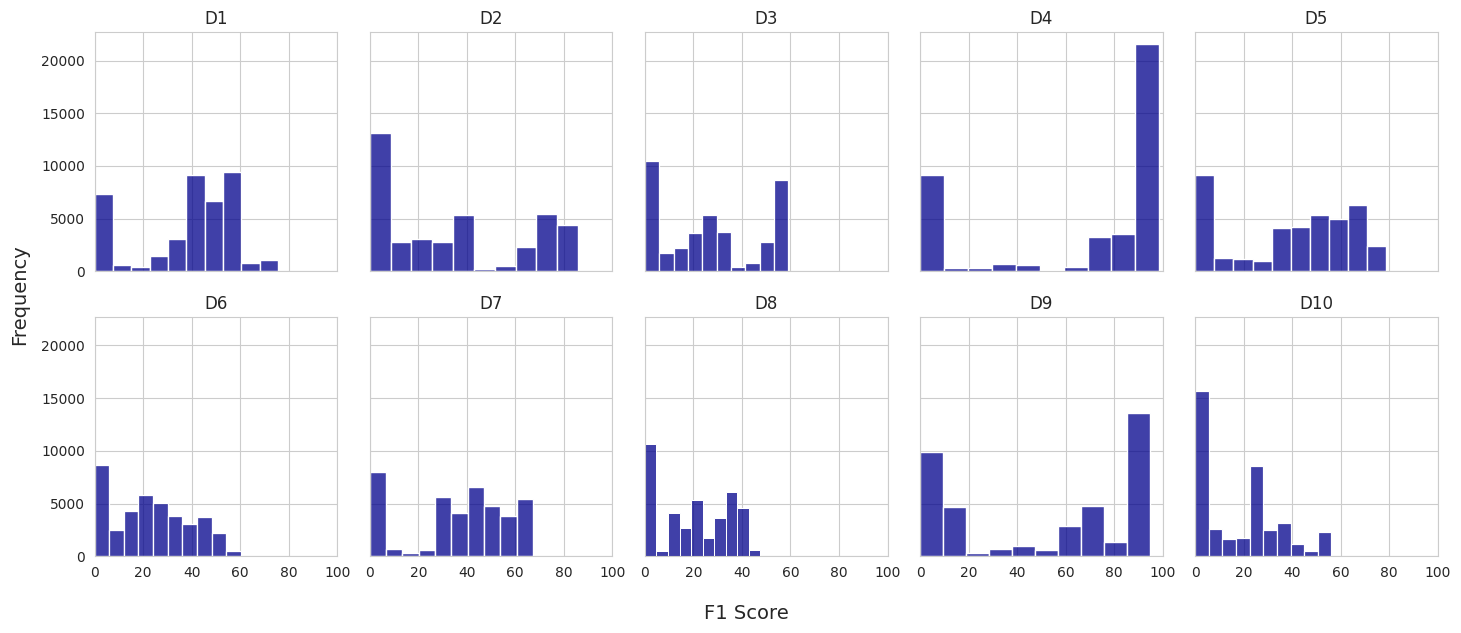
\includegraphics[width=0.97\linewidth]{Nikoletos-paper/figures/predictions/f1_score_distribution.png}
    % \vspace{-10pt}
    \caption{The distribution of F1-scores for the end-to-end ER pipeline of Figure~\ref{fig:eeter_pipeline}, when applying the 39,900 different configurations of Table~\ref{tab:parameter-values} to the 10 real-world datasets of Table~\ref{tab:dataset-specs}.}
    \label{fig:f1_boxplot_all}
    % \vspace{-14pt}
\end{figure*}

This is illustrated in Figure \ref{fig:f1_boxplot_all}, which demonstrates the range of F1 scores over 10 established real-world datasets 
%in Table \ref{tab:dataset-specs} 
(see Section \ref{sec:expSetup} for more details). {There is a separate diagram (i.e., bar chart) for each dataset. In each bar chart, the horizontal axis corresponds to the F-Measure of 
%For each dataset, we assessed the performance of 
the state-of-the-art end-to-end ER pipeline in Figure \ref{fig:eeter_pipeline} \cite{DBLP:journals/pvldb/ZeakisPSK23}, while the vertical axis corresponds to the frequency of the respective interval of F1 scores. This frequency stems from the grid search we applied to the configuration parameters of the selected ER pipeline: as shown in Table~\ref{tab:parameter-values}, grid search yields 39,900 different configurations (see Section \ref{sec:eteer_pipeline} for more details). Thus, there are 39,900 F1 scores per dataset, with their distribution illustrated through the bar charts.
%In fact, there is a separa we applied  . In total, we applied 39,900 different configurations per dataset, with 
We observe that} their performance exhibits a large deviation between the maximum and the minimum F1 score: 
in most datasets, the vast majority of configurations covers all values in $[0,50]$, while in datasets $D_4$ and $D_9$, the range is even larger, going up to 100 (both datasets contain unambiguous bibliographic data like author names and publication titles that ensure high performance for a large portion of configurations). This indicates significant sensitivity to the configuration parameters of the ER pipeline, with most options typically leading to rather low effectiveness. 

These settings highlight the importance of fine-tuning end-to-end ER pipelines. However, choosing the right configuration is a non-trivial task that requires time-consuming trial-and-error experimentations even for experts. To address this problem, we formulate parameter fine-tuning as a regression task over a large search space and leverage established sampling-based techniques for hyperparameter optimization. We experimentally demonstrate that these techniques are able to propose parameter configurations that approximate the optimal performance by curtailing the search space by orders of magnitude -- with fewer than 100 trials.

{
Note that the need for configuration fine-tuning applies also to the latest works on ER, which leverage LLMs for Entity Matching. In fact, LLM-based Matching comes in various forms that range from zero- and few-shot prompts \cite{DBLP:conf/edbt/PeetersSB25}, to SELECT prompts \cite{DBLP:conf/coling/WangCLCHSWZ25} and fine-tuning \cite{DBLP:journals/corr/abs-2409-08185}. These solutions involve numerous parameters (e.g., the selection criteria for the examples in few-shot prompting or fine-tuning), but apply only to the Verification part of end-to-end ER solutions (see Figure \ref{fig:eeter_pipeline}). This means that they disregard the preceding step of Filtering, which has a decisive impact on the candidate pairs processed by the matching algorithm. Most importantly, there is no clear winner among the plethora of proposed solutions (e.g., there is no comparison between the SELECT prompts and the fine-tuned LLMs), while their use in practice is quite challenging \cite{DBLP:conf/edbt/PeetersSB25,DBLP:conf/coling/WangCLCHSWZ25,DBLP:journals/corr/abs-2409-08185}: they have considerable hardware requirements, typically running on top of GPUs equipped with large VRAM, with their time efficiency being very low (i.e., high run-times). For these reasons, we exclusively consider the pipeline in Figure \ref{fig:eeter_pipeline}, which balances high effectiveness with high time efficiency by leveraging one of the top-performing pre-trained language models \cite{DBLP:journals/pvldb/ZeakisPSK23}.
}

%that are aware of the ground truth. 
Another obstacle in practical ER applications is the lack of ground truth with correct matches that allows for
%setting, though, the end user does not have a ground truth of (otherwise, the ER problem is solved/not needed for that dataset) so they cannot even 
evaluating the performance of different configurations automatically.
%, i.e., without costly
%, other than a brief and unreliable 
%manual inspections. 
%In the context of PPC's digital transformation, one of the main targets is the transition from legacy systems to high-end information systems such as ERP, CRMs etc. This requires deduplicating a series of databases that contain customer, employee and supplier data and were kept isolated in different departments. This data, though valuable, exhibit high levels of noise and of missing values, even identification attributes like person Ids. To leverage this legacy data, we need to democratize ER by enabling data scientists of any experience, even novice ones, to apply effective end-to-end ER pipelines. This can be accomplished by automating the parameter configuration of ER pipelines. 
%To this end, 
To address this task, we formulate a regression task, where the input comprises a feature vector describing the combination of a dataset and an ER pipeline configuration, while the output is the corresponding F1 score. In this context, datasets with known ground truth act as training instances, while datasets without a ground truth form the testing instances. We apply the trained model to all instances of a dataset without a ground truth and the one maximizing the expected F1 score indicates the most suitable parameter configuration. Using the end-to-end ER pipeline of Figure \ref{fig:eeter_pipeline}, we apply existing techniques for each part of this regression model: feature engineering is based on dataset profiling, the instances are generated by grid search, sampling-based algorithms, or both, and the learning process is carried out by two established approaches with integrated feature selection, namely Random Forests and AutoML. Our extensive experimental evaluation demonstrates which combination of these techniques yields the best performance.
%in terms of effectiveness and time efficiency.
%By estimating the 
%propose an auto-configurable ER pipeline that receives as input a dataset, optionally along with a partial ground truth of correct matches, 
%very small number of labeled matches, 
%and returns ER results after automatically deciding which configurations
%setting 
%are the most suitable for the task at hand.
%dataset. 
%Internally, our approach leverages a state-of-the-art end-to-end ER pipeline that uses language models for blocking and matching \cite{DBLP:journals/pvldb/ZeakisPSK23}. Its configuration parameters include the number of candidates per entity, the language model that creates the embedding vector of each entity, the clustering algorithm and the similarity threshold. Using a training set extracted from real datasets with a complete ground truth, AutoER applies AutoML techniques 
%or individual regression algorithms 
%to fine-tune these four parameters by selecting the best value in their domain.
%one among XXXXX different configurations. 
%We experimentally show that in almost all cases, AutoER yields results that are very close to the best obtainable ones, as they are determined via grid search over a large configuration space.

In summary, this works makes the following contributions:
%of this work are the following: 
\begin{itemize}[leftmargin=*]
    \item We define two problems for the automatic configuration of end-to-end ER pipelines: one assuming a ground truth and another one assuming no ground truth information. {To the best of our knowledge, there is no prior definition of relevant problems in ER literature.}
    \item We show how both problems can be addressed by existing techniques that have never been applied to the task of automatic ER pipeline configuration. {In fact, we are the first to apply sampling techniques to address the ground truth-aware auto-configuration problem, evaluating their relative performance in the context of ER. Note that ER differs from other learning tasks as it is impossible to materialize all negative instances (i.e., non-matching pairs), due to their quadratic space complexity. For this reason, the performance of the sampling techniques is exclusively guided by the F-Measure of the entire end-to-end ER pipeline. We are also the first to 
    model the regression-based solution to the ground truth-agnostic auto-configuration problem. We combine existing features with new ones in the feature engineering part of our solution, while exploring a rich diversity of strategies for instance generation. }
    %propose AutoER, a framework that solves both problems by automatically configuring a state-of-the-art end-to-end ER pipeline leveraging language models for blocking and matching. %based on  predicts the best ER pipeline configurations for a given dataset, with or without a known ground truth.
    %\item AutoER can operate even without a ground truth, but it can also exploit a small set of labeled matches and quickly find the best configuration. 
    \item We perform extensive experimental evaluations over 11 established, real-world datasets 
    %with real data 
    to identify the best solutions per problem.
    %demonstrates the high performance of our approaches in both problems
    %39,900 possible configurations generated by grid-search in 10 established datasets. including Z language models, ... , and YYY widely used datasets,} compared against state-of-the-art methods. 
    %\item 
\end{itemize}

We have open-sourced our code with a permissive license on Github: \underline{https://github.com/AI-team-UoA/AutoER}.

\section{Problem Definition}\label{sec:problem}

\begin{figure}[t]
    \centering
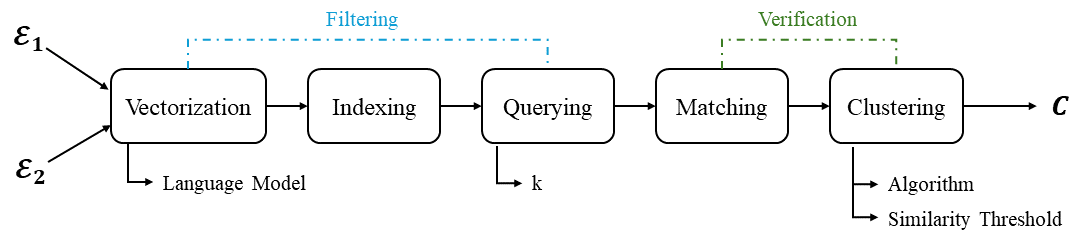
\includegraphics[width=0.97\linewidth]{figures/pyjedai/pipeline-AutoER.png}
    % \vspace{-20pt}
    \caption{The ETEER pipeline considered in this work.}
    \label{fig:eeter_pipeline}
    % \vspace{-12pt}
\end{figure}

%In this section, we describe the problem that this paper tackles, which is end-to-end entity resolution, namely ETEER. We define two variations of this problem, depending on whether ground truth knowledge is available or not. 

Let an \emph{entity collection} $\mathcal{E}$ be a set of entity descriptions, where each description (also called ``entity'' for brevity)
%, we will also refer to entity descriptions, simply as .} 
is a set of attribute-value pairs representing a real-world entity (e.g., an entity description can be a database record, a row in a csv file, a json element or an ontology class instance). 

End-to-end ER (ETEER) is the problem of receiving one or more entity collections and returning a set of entity \emph{clusters}, with each cluster corresponding to a set of entity descriptions that refer to the same real-world entity. 
%Although ER can be generalized to receive as input one (Dirty ER~\cite{DBLP:journals/pvldb/HassanzadehCML09}), two (Clean-Clean ER~\cite{DBLP:journals/vldb/PapadakisETHC23}), or more than two (Multi-Source ER~\cite{DBLP:conf/esws/SaeediPR20,DBLP:conf/adbis/SaeediPR17}) entity collections, in this work, we will assume the case of two clean (i.e., duplicate-free) entity collections $\mathcal{E}_1$ and $\mathcal{E}_2$ that need to be resolved. Our definitions and methodology can be easily generalized to cover all other cases. 

More formally:
% \begin{problem} 
% \label{pr:eteer}
% Given two entity collections $\mathcal{E}_1$ and $\mathcal{E}_2$, cluster them into a set of disjoint clusters $\mathcal{C}$, such that $\forall c_i, c_j \in \mathcal{C}\;  c_i \cap c_j = \emptyset$, with $i \neq j$, 
% and $c_i \subset \mathcal{E}_1 \cap \mathcal{E}_2$, if $|c_i|=2$, or $c_i \subset \mathcal{E}_1 \cup \mathcal{E}_2$, if  $|c_i|=1$.
% \end{problem}
\vspace{4pt}
\begin{definition}[End-to-end Entity Resolution (ETEER)]\label{def:eteer}
Given two entity collections $\mathcal{E}_1$ and $\mathcal{E}_2$, return a set of disjoint clusters $\mathcal{C}$, such that 
$\bigcup_{c_l \in \mathcal{C}}c_l = \mathcal{E}_1 \cup \mathcal{E}_2$, and
$\forall c_l \in \mathcal{C}, 
 e_i \in \mathcal{E}_1 \cap c_l, e_j \in \mathcal{E}_2 \cap c_l \Rightarrow e_i \equiv e_j$, 
where $e_i \equiv e_j$ denotes that the two entity descriptions~\emph{match} {(i.e., they correspond to identical real-world objects)}.
%, referring to the same real-world entity.
\end{definition}
\vspace{4pt}

% \begin{problem} 
% \label{pr:eteer_alternative}
% \comments{[alternative def]}
% Given two entity collections $\mathcal{E}_1$ and $\mathcal{E}_2$, cluster them into a set of disjoint clusters $\mathcal{C}$, such that 
% $\bigcup_{c_i \in \mathcal{C}}c_i = \mathcal{C}$, and
% $\forall c_i \in \mathcal{C}, 
% |c_i|=2$, if $c_i \subseteq \mathcal{E}_1 \cap \mathcal{E}_2$, otherwise, $|c_i|=1$. 
% \end{problem}

This definition applies to Record Linkage \cite{DBLP:books/daglib/0030287}, also known as Clean-Clean ER~\cite{DBLP:journals/vldb/PapadakisETHC23}, where $\mathcal{E}_1$ and $\mathcal{E}_2$ are individually duplicate-free, but overlapping, sharing some entities. In this setting, each cluster contains either a single  entity from one entity collection, or 
%two entities,
one from each collection. Definition~\ref{def:eteer} can be easily generalized to Dirty ER \cite{DBLP:journals/pvldb/HassanzadehCML09}, also known as Deduplication \cite{DBLP:books/daglib/0030287}, where the input comprises a single entity collection with duplicates in itself. In this case, the resulting clusters are also disjoint, but there is no limit on their size, i.e., the number of entities they contain. It can also be generalized to the case of Multi-Source ER \cite{DBLP:conf/esws/SaeediPR20,DBLP:conf/adbis/SaeediPR17}, where the input comprises multiple, duplicate-free entity collections. This setting requires that each cluster cannot contain more than one entity from the same collection. 

% The problem of Definition~\ref{def:eteer} is typically solved through an ETEER pipeline, denoted by $w(\mathcal{E}_1, \mathcal{E}_2)$, whose \underline{effectiveness} is assessed with respect to: i) \textit{Precision}, which is is the portion of pairs in $\mathcal{C}$ that are indeed matching, ii) \textit{Recall}, which is is the portion of pairs in $\mathcal{D}$ that co-occur in some cluster of $\mathcal{C}$, where $\mathcal{D}$ denotes the set of duplicate entities, and iii) \textit{F-Measure}, which is the harmonic mean of Precision and Recall. The \underline{time efficiency} of $w(\mathcal{E}_1, \mathcal{E}_2)$ is measured in terms of the overall run-time, i.e., the time intervenes between receiving $\mathcal{E}_1$ and $\mathcal{E}_2$ and producing $\mathcal{C}$.

The problem of Definition~\ref{def:eteer} is typically solved through an \emph{ETEER pipeline}, also called \emph{workflow}, denoted by $w(\mathcal{E}_1, \mathcal{E}_2)$. This involves a series of processing steps, which potentially require the configuration of some parameters. More formally:
\vspace{4pt}
\begin{definition}[ETEER Pipeline]
An ETEER Pipeline $w(\mathcal{E}_1, \mathcal{E}_2) = (S, P, V)$ is a series of processing steps $S = s_1, s_2, \ldots, s_n$ for solving ETEER, with each processing step $s_i$ potentially requiring the configuration of some parameters $P_i = p_1^i, p_2^i, \ldots, p_m^i$, and with each parameter $p_j^i$ accepting a set of possible values $V_j^i$.
\end{definition}
\vspace{4pt}

Following the previous definition, we 
%will sometimes simply 
call the set $P = \bigcup\limits_{i \in [1..n]}
P_i$ \emph{configuration parameters} and 
%we will also simply call 
the set $V = \bigcup\limits_{P_i \in P, p_j \in P_i}V_j^i$ as \emph{configuration values} or \emph{possible values}.

The \underline{effectiveness} of an ETEER pipeline is assessed in terms of precision, recall, and F1-score, with respect to the ground truth of known matches $\mathcal{D}$. In more detail,
\textit{precision} is the portion of clusters in $\mathcal{C}$ which contain a pair of entities that also appears in $\mathcal{D}$; 
\textit{recall} is the portion of pairs in $\mathcal{D}$ that co-occur in some cluster of $\mathcal{C}$;
\textit{F1-score} is the harmonic mean of precision and recall.

The \underline{time efficiency} of an ETEER pipeline can be measured in terms of the 
overall runtime, i.e., the time between receiving $\mathcal{E}_1$ and $\mathcal{E}_2$ and producing $\mathcal{C}$. 
%Given that we are interested in finding the best configuration for a fixed ETEER pipeline, we will focus more on measuring time efficiency of AutoER in terms 
In this work, we also consider
%Another crucial aspect is
the \emph{search time}, i.e., the time needed to %produce a the suggested 
recommend configuration values.


In this context, we address two problems for fine-tuning ETEER pipelines, based on whether a ground truth is available (Problem~\ref{pr:pr1}) or not (Problem~\ref{pr:pr2}).
%for configuration tuning. 
%Such a (subset of the) ground truth is also known as ``seed alignment'' and is used for training entity alignment models~\cite{DBLP:journals/datamine/FanourakisEKC23,DBLP:journals/pvldb/SunZHWCAL20}. 
For the evaluation, we always use the ground truth of known matches $\mathcal{D}$. In Problem~\ref{pr:pr1}, we also use $\mathcal{D}$
%a portion of the ground truth 
for tuning the configuration parameters, unlike Problem~\ref{pr:pr2}.
More formally:
%, we do not use any portion of the ground truth.

% $\bullet$ \textit{Specified ETEER pipeline and ground truth.} The goal is to fine-tune a specific ETEER pipeline provided that some subset of the golden standard of real matches is available. This task can be formalized as follows:
% \Figure[t!](topskip=0pt, botskip=0pt, midskip=0pt, wid){figures/pyjedai/pipeline-AutoER.png}
% {The ETEER pipeline considered in this work.}
\vspace{4pt}
\begin{problem}\label{pr:pr1}
Given an ETEER pipeline $w(\mathcal{E}_1, \mathcal{E}_2)$ for two entity collections $\mathcal{E}_1$ and $\mathcal{E}_2$, along with a subset of the ground truth of matches $\mathcal{D}' \subseteq \mathcal{D}$, return the configuration values $V' \subseteq V$ of $w(\mathcal{E}_1, \mathcal{E}_2)$ that maximize the effectiveness of $w(\mathcal{E}_1, \mathcal{E}_2)$ in terms of F1-score, while minimizing the search time.
\end{problem}
\vspace{4pt}
For the returned configuration values $V'$, it holds that $|V'| = |P|$, i.e., one value should be returned for each configuration parameter.

The na\"ive approach is to apply \textit{grid search}, considering all meaningful values for all configuration parameters in the specified pipeline. However, this is impractical and time-consuming, due to the enormous configuration space.
%even for simple ETEER pipelines, because they typically involve numerous configuration parameters with large domains. Therefore, 
More advanced algorithms for configuration optimization are required to effectively restrict the search to a small portion of the configuration space.
%extremely large search space of configuration parameters. 

% $\bullet$ \textit{Specified ETEER pipeline without ground truth.} 

A more difficult variation of the first problem is to fine-tune a specific ETEER pipeline without having any portion of the real matches $\mathcal{D}$ provided as input. This task can be formalized as follows:

\vspace{4pt}
\begin{problem}
\label{pr:pr2}
Given an ETEER pipeline $w(\mathcal{E}_1, \mathcal{E}_2)$ for two entity collections $\mathcal{E}_1$ and $\mathcal{E}_2$, {without relying on their ground truth}, return the configuration values $V' \subseteq V$ of $w(\mathcal{E}_1, \mathcal{E}_2)$ that maximize the effectiveness of $w(\mathcal{E}_1, \mathcal{E}_2)$ in terms of F1-score, while minimizing the search time.
% Given an ETEER pipeline $w(\mathcal{E}_1, \mathcal{E}_2)$ and two entity collections, $\mathcal{E}_1$ and $\mathcal{E}_2$, optimize the configuration parameters of $w(\mathcal{E}_1, \mathcal{E}_2)$ so as to maximize its effectiveness in terms of F-Measure, while minimizing the search time.
\end{problem}
\vspace{4pt}

To the best of our knowledge, no prior work on ER examines these tasks, even though both can be solved by existing techniques. 
\section{ETEER pipeline}\label{sec:eteer_pipeline}

We now present the ETEER pipeline that we use to address
%will be used in our solutions to 
Problems~\ref{pr:pr1} and \ref{pr:pr2}. 
%As is common in the literature, our ETEER pipeline 
Due to the quadratic complexity of the brute-force approach, it consists of two steps:
\begin{itemize}[leftmargin=*]
    \item \emph{Filtering}, which reduces the computational cost by identifying a set of promising \emph{candidate pairs} to be matched.
    \item \emph{Verification}, which analytically examines each pair of candidates.
\end{itemize}

Based on a recent experimental study \cite{DBLP:journals/pvldb/ZeakisPSK23}, our solution relies on the ETEER pipeline shown in Figure~\ref{fig:eeter_pipeline}, which leverages language models. This approach not only combines high effectiveness with high time efficiency, but also requires the fine-tuning of a limited set of configuration parameters.

%\section{Methodology}\label{sec:methodology}
%\comments{Wouldn't it be better to state it like With and Without Ground-truth file?}

%\guides{Here we need an overview of the approach and how it is presented in that section, say that we will present the parameters to be configured next, say that we can handle both cases when we have and when we don't have a ground truth and also say what difference it makes in our approach, i.e., HOW we handle those two cases.}

%\begin{figure*}[t]
%    \centering
%    \includegraphics[width=0.8\linewidth]{figures/pyjedai/Allpipelines.PNG}
%    \caption{PyJedAI pipelines. (a) Similarity Joins pipeline (b) Blocking-based pipeline (c) Nearest Neighbors using Pre-trained LMs pipeline.}
%    \label{fig:pipelines}
%\end{figure*}

The first step of this ETEER pipeline is Vectorization, where the input entities are transformed into embedding vectors using pre-trained LMs, either static ones like Word2Vec \cite{DBLP:journals/corr/abs-1301-3781} and GloVe \cite{DBLP:conf/emnlp/PenningtonSM14}, or dynamic ones, like BERT \cite{DBLP:conf/naacl/DevlinCLT19} and SentenceBERT~\cite{DBLP:conf/emnlp/ReimersG19}.
% available via PyTorch, 
The former are context-agnostic, assigning each word to the same vector regardless of its context, while the latter are context-aware, generating different embeddings for different meanings of the same word (e.g., trunk as part of a tree or an elephant). Therefore, selecting the appropriate language model is crucial for achieving good results. Following \cite{DBLP:journals/pvldb/ZeakisPSK23}, we restrict our configurations to five state-of-the-art SentenceBERT models and two static models, listed in Table \ref{tab:parameter-values} 
%parameter our study aims to configure 
\textbf{(Parameter: LM)}. 
%The reason is that the 
Pre-trained BERT models yield scores of very low distinctiveness, failing to distinguish between matching and non-matching pairs, unless
%in case 
they are fine-tuned \cite{DBLP:journals/pvldb/ZeakisPSK23}.
%Overall, the four SBERT models listed in  are considered - 
Describing them in more detail goes beyond the scope of this work.

\begin{table}[t]
    \centering
    \caption{Configuration parameters and their domains.}
    % \vspace{-8pt}
    \label{tab:parameter-values}
    \begin{tabular}{|p{3cm}|p{4.5cm}|}
        \hline
         \multicolumn{1}{|c|}{\textbf{Parameters ($P$)}} & \multicolumn{1}{|c|}{\textbf{Possible values ($V$)}} \\ \hline
        Language model (LM) & smpnet, S-GTR-T5, sdistilroberta, sminilm, sent\_glove, fasttext, word2vec \\ \hline
        $k$ & $[1, 100]$ with a step of 1\\ \hline
        Clustering algorithm & Unique Mapping Clustering (UMC), Kiraly Clustering (KC), Connected Components (CCC) \\ \hline
        Similarity Threshold & $[0.05, 0.95]$ with a step of 0.05\\ \hline
    \end{tabular}
\end{table}

Note that we apply a schema-agnostic serialization scheme, which simply concatenates all attribute values into a sentence describing each entity (i.e., all attribute names are excluded). This way, we inherently address noise in the form of misplaced values, while also achieving very high performance under versatile settings~\cite{DBLP:journals/pvldb/ZeakisPSK23}.

The second step is Indexing. It receives as input all embedding vectors of $\mathcal{E}_1$ and organizes them in a data structure that facilitates their retrieval in descending distance from a given query, i.e., an embedding vector of $\mathcal{E}_2$. 
%Each entity is transformed into an embedding vector, and these embeddings are then indexed in the ep. 
Based on a recent experimental study \cite{DBLP:journals/is/AumullerBF20}, we employ 
%Queries are performed on this indexing module using 
FAISS \cite{DBLP:journals/corr/abs-2401-08281} for this purpose, due to its excellent balance between effectiveness and time efficiency.
%, a vector similarity search tool developed by Meta. 
We actually use a FAISS configuration that returns exact results, which does not require parameter tuning.\footnote{{The exact functionality of FAISS provides the real $k$-nearest neighbors in terms of cosine similarity, whereas the approximate functionality achieves a lower run-time at the cost of returning candidates that are not among the $k$ most similar ones.}}
%No parameter needs to be configured in this step, given that we employ the configuration returning the exact results.
For datasets with more than 10,000 entities, the approximate search should be applied to ensure high time efficiency, but its configuration is also straightforward.\footnote{For more details, please refer to \underline{https://github.com/facebookresearch/faiss/wiki/Guidelines-to-choose-an-index}.}

The third step is Querying. It receives as input all embedding vectors of $\mathcal{E}_2$ and uses each vector/entity as a query to the FAISS index. The result of each query consists of the $k$ most similar entities from $\mathcal{E}_1$ in terms of cosine similarity. The $k$ parameter is the sole configuration parameter of this step, playing a major role in the performance of ETEER. The higher the value of $k$, the higher the filtering recall, at the cost of lower precision. Note that the filtering recall sets the upper bound of the overall ETEER recall, given that the subsequent steps do not detect new matches. Hence, $k$ is the second configuration parameter of the pipeline \textbf{(Parameter:~$\mathbf{k}$)}.

%Note also that t
The first three steps together implement the Filtering approach, which reduces the computational cost to the $k$ most similar $\mathcal{E}_2$ entities per $\mathcal{E}_1$ entity. %This means that 
It receives as input the entity collections and returns as output a set of candidate pairs.% $P$.

%\comments{We need to be consistent in the description here and the steps shown in the figure. E.g., Which step or series of steps corresponds to the $kNN$ step mentioned here? In the text, we skip the Entity Matching step and go directly to clustering. Filtering is only shown in the figure, but never explained in text}

Subsequently, the set of candidate pairs 
%$P$ 
is transformed into a \textit{similarity graph} {by Matching, the fourth step of our ETEER pipeline, which estimates the similarity score between all candidate pairs. In the similarity graph, the nodes correspond to entities, while the edges connect the candidate pairs, with their weights indicating their similarity, i.e., the cosine similarity returned by FAISS.} 
%where every node is an entity and every edge represents a candidate pair, weighted according to . 
Note that the similarity graph is bipartite in the Record Linkage settings we are considering. 
%This transformation is carried out by Matching,  {
No configuration parameter is involved in this process. 

The final step of the ETEER pipeline is Clustering, which applies bipartite graph matching algorithms to the similarity graph generated by the previous step. Based on a recent experimental study~\cite{DBLP:journals/vldb/PapadakisETHC23}, three established algorithms combine high time efficiency with high effectiveness: Connected Components (i.e., transitive closure), Unique Mapping Clustering \cite{DBLP:conf/kdd/Lacoste-JulienPDKGG13}, and Kiraly Clustering~\cite{DBLP:journals/algorithms/Kiraly13} \textbf{(Parameter: Clustering)}.\footnote{A more detailed description of their functionality lies out of the scope of this work, but the interested reader can refer to \cite{DBLP:journals/vldb/PapadakisETHC23} and the original publications of each algorithm.}
All algorithms are configured by 
%Perhaps the most important parameter is 
a similarity threshold \textbf{(Parameter: Threshold)}, which prunes the edges with a lower weight.

Note that Clustering is the only step that 
%differs, 
depends on the type of ER task at hand. In the case of Dirty ER, the state-of-the-art unconstrained algorithms for undirected similarity graphs are experimentally evaluated in \cite{DBLP:journals/pvldb/HassanzadehCML09}. Among them, Markov Clustering exhibits a performance that is robust to noise and portion of duplicates, while achieving high effectiveness and scalability. For Multi-source ER, the main clustering techniques are evaluated in \cite{DBLP:journals/csimq/SaeediNPR18}, with CLIP~\cite{DBLP:conf/esws/SaeediPR18} outperforming all others -- CLIP essentially generalizes Unique Mapping Clustering to Multi-source~ER.

The configuration space of our pipeline is summarized in Table~\ref{tab:parameter-values}. Note that grid search should consider 39,900 different parameter combinations per dataset in order to maximize the corresponding F1 (7 pre-trained language models $\times$ 100 values for $k$ $\times$ 3 clustering algorithms $\times$ 19 values for similarity threshold). Our goal is to experimentally evaluate algorithms that converge to the maximum performance, while minimizing the trials in this search space.
%\vspace{-8pt}
\section{Tackling Problem 1}
\label{sec:problem-1}
%\vspace{-4pt}

Fine-tuning an ETEER pipeline based on the ground truth comprising all duplicate pairs is similar to hyperparameter fine-tuning in Machine and Deep Learning models \cite{DBLP:journals/ijon/YangS20}. The only difference is the form of the data: in the latter case, the data comes in the form of positive and negative labelled instances, which is not possible in ETEER, due to the extremely large number of pairs that arise even from relatively small datasets with few thousand entities in $\mathcal{E}_1$ and $\mathcal{E}_2$. Besides, the number of positive pairs grows linearly with respect to the number of given entities, while all other pairs are negative, with their number growing quadratically \cite{DBLP:journals/pvldb/GetoorM12}. Therefore, instead of enumerating and labelling all possible pairs in the Cartesian product of $\mathcal{E}_1 \times \mathcal{E}_2$, hyperparameter fine-tuning is guided by the F1-score corresponding %to the matches generated by each 
to each parameter configuration of the ETEER pipeline to be fine-tuned. This is the only change that needs to be applied to existing algorithms for hyperparameter fine-tuning, yet they have not been applied before to Problem 1.

Typically, hyperparameter fine-tuning is carried out by \emph{sampling techniques}, which aim at optimizing the balance between effectiveness and time efficiency:  
%two goals of auto-configuration \cite{OPTUNA}: ($i$) 
their goal is to maximize efficiency by reducing the search space to the most promising subset of configuration parameters, without leaving out the ones maximizing effectiveness~\cite{OPTUNA}. 
%in the configuration strategy that
%is the process of 
%determines the (sub)set of parameters that are worth investigating \cite{OPTUNA}.
%, and ($ii$) the efficiency of performance estimation strategy, that estimates the value that a set of configurations will produce, based on learning curves, and finally determines the set of parameters that should be discarded. 
These sampling techniques are categorized into two main types: 
the \textit{relational} ones select the next set of configuration parameters based on the correlations between them, while the \textit{independent} ones disregard inter-parameter correlations.
%(ii) \textit{Independent sampling} selects the next configuration parameters regardless of correlations between them.

In this work, we consider the following state-of-the-art sampling algorithms \cite{OPTUNA}, which cover both types of sampling techniques:
%three are independent and one is relational (assume that $d$ is the dimension of the search space and $n$ is the number of finished trials): 

(1)  \emph{RandomSampler} \cite{QMCSampler}. As its name suggests,  
    %with %complexity of $O(d)$, is an independent sampling technique, where 
    hyper-parameter values are chosen randomly from the specified search space. This is an independent method that does not use any prior knowledge or adaptive mechanisms to guide the search process. Instead, it 
    %relies on randomness to 
    explores the search space in a purely stochastic manner, i.e.,
    %. Random sampling achieves high efficiency in many cases because 
    each point in the search space has an equal probability of being explored. This approach results in a uniform coverage of the search space. Even in high-dimensional spaces, random sampling is capable of identifying near-optimal configurations with fewer trials, especially when compared to the grid search approach. 
    %Another advantage is its high time efficiency, given that its time complexity of is $O(d n)$.

(2) Tree-structured Parzen Estimator (\emph{TPESampler}) \cite{TPE1, TPE2, TPE3}.
    %, with complexity of $O(d*n*log_2n)$, uses the TPE (Tree-structured Parzen Estimator) algorithm and utilizes independent sampling \cite{TPE1, TPE2, TPE3}. 
    During each trial for every parameter, this independent algorithm fits two Gaussian Mixture Models (GMMs): \( l(x) \) to the set of parameter values with the best objective outcomes, and \( g(x) \) to the remaining parameter values. It then selects the parameter value \( x \) that maximizes the ratio \( l(x) / g(x) \).  In other words, TPESampler models the distribution of good and bad hyperparameters using non-parametric density estimators, focusing on promising regions of the search space. By iteratively updating these models based on observed results, TPESampler may need more trials to explore potentially optimal areas, but typically exhibits better search performance than grid search and RandomSampler. 
    %, where $d$ stands for the dimensionality of the search space and $n$ for the number of completed trials. 

(3) Quasi Monte Carlo Sampler (\emph{QMCSampler}) \cite{QMCSampler}. This independent approach uses quasi-random methods, specifically low-discrepancy sequences, to enhance the efficiency of hyperparameter optimization by ensuring uniform coverage of the search space. Unlike RandomSampler, which can have uneven distribution, low-discrepancy sequences spread points more evenly, avoiding clumps and gaps. This uniformity increases the probability of finding optimal hyperparameters with fewer trials, particularly in high-dimensional settings where important dimensions need adequate sampling. 
%, where $d$ denotes the search space dimensionality and $n$ the number of executed trials.

(4) Gaussian Process-based Bayesian Sampler (\emph{GPSampler}) \cite{NIPS2012_GPSampler, QMCSampler}. This is a relational sampler that fits a Gaussian process to the objective function and optimizes the acquisition function to suggest the next set of parameters. First,
    %Bayesian optimization methods, in general, first 
    it constructs a probabilistic model of the objective function using a Gaussian process and then it exploits this model to estimate the most promising regions in the search space. 
    %The GPSampler uses a Gaussian process to represent the probabilistic distribution of the objective function, providing flexibility and adaptability. Among various acquisition functions, 
    To this end, it employs the log expected improvement 
    %(logEI) 
    in combination with QMCSampler
    %Quasi-Monte Carlo (QMC) sampling 
    to optimize the acquisition function (note that in Bayesian optimization, the acquisition function tackles the exploration-exploitation trade-off, efficiently providing numerical estimations that indicate the most promising configuration parameters to be tested \cite{DBLP:conf/nips/WilsonHD18}).
    %Gaussian process-based Bayesian approaches, have proven 
    Typically, GPSampler is highly effective in hyperparameter optimization,
    %(HPO) problems, 
    as it leverages the dependencies between hyperparameters and avoids redundant trials, due to their probabilistic estimation of the objective function \cite{NIPS2012_GPSampler, QMCSampler}. 

Regarding the time complexity \textit{per trial} of these samplers, we use $d$ for the dimensionality of the search space {(i.e., the four parameters in Table \ref{tab:parameter-values} that have to be configured in order to fine-tune the ETEER pipeline in Figure \ref{fig:eeter_pipeline})} and $n$ for the number of completed trials. The most efficient algorithm is RandomSampler, with $O(d)$, followed by QMCSampler with $O(d n )$, TPESampler with $O(d n logn)$ and GPSampler with $O(n^3)$ -- for more details, please refer to {\footnotesize \underline{https://optuna.readthedocs.io/en/stable/reference/samplers/index.html}}.

To the best of our knowledge, none of these algorithms has been applied to fine-tuning ETEER pipelines, addressing Problem 1. More specifically, each algorithm is applied to Problem 1 as follows: 
\begin{enumerate}[leftmargin=*]
    \item It receives $V$ as input, i.e., the domain of each configuration parameter, along with the maximum number of trials.
    \item In each trial, it selects a value for each configuration parameter.
    \item The resulting ETEER pipeline is applied to the given dataset to estimate its performance with respect to F1-score, using the available ground truth.
    \item After consuming the budget of trials, the configuration values $V' \subseteq V$ maximizing F1-score are returned as output.
\end{enumerate}



\begin{figure*}[h!]
    \centering
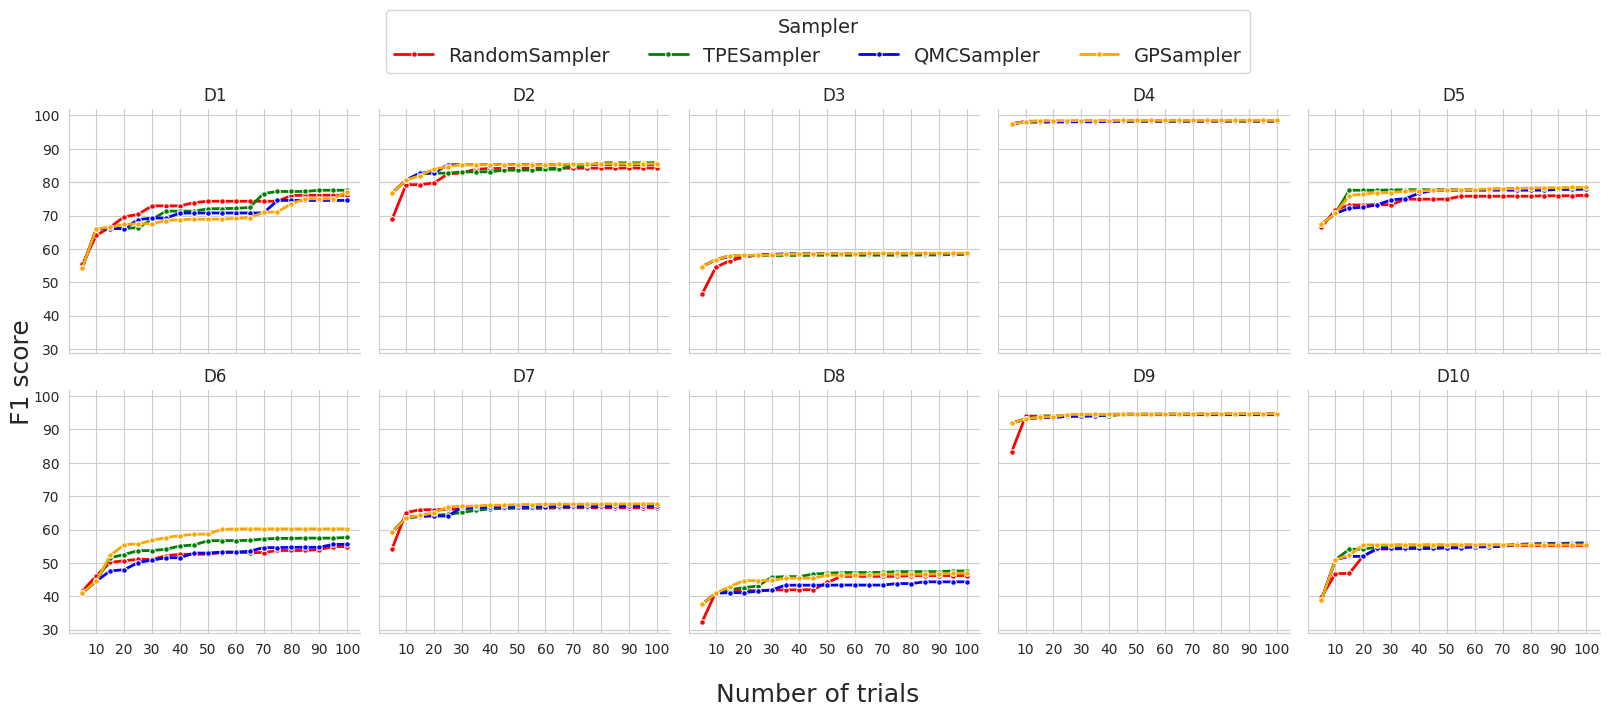
\includegraphics[width=0.97\textwidth]{figures/predictions/f1_convergence_plots.png}
    % \vspace{-10pt}
    \caption{F1-score of the sampling-based search algorithms in Section \ref{sec:problem-1} as the number of trials increases from 5 to 100.}
    \label{fig:samplers-convergence-avg-f1}
\end{figure*}

\section{Experimental Evaluation - Problem 1}\label{sec:experiments-p1}
%In this section, we first present our experiments for tackling Problem~\ref{pr:pr1} (Section~\ref{sec:problem-1}), and then by utilizing all the results produced we proceed on showing the results for tackling Problem~\ref{pr:pr2} (Section~\ref{sec:problem-2}).


%\begin{figure}[t]
%    \centering
%    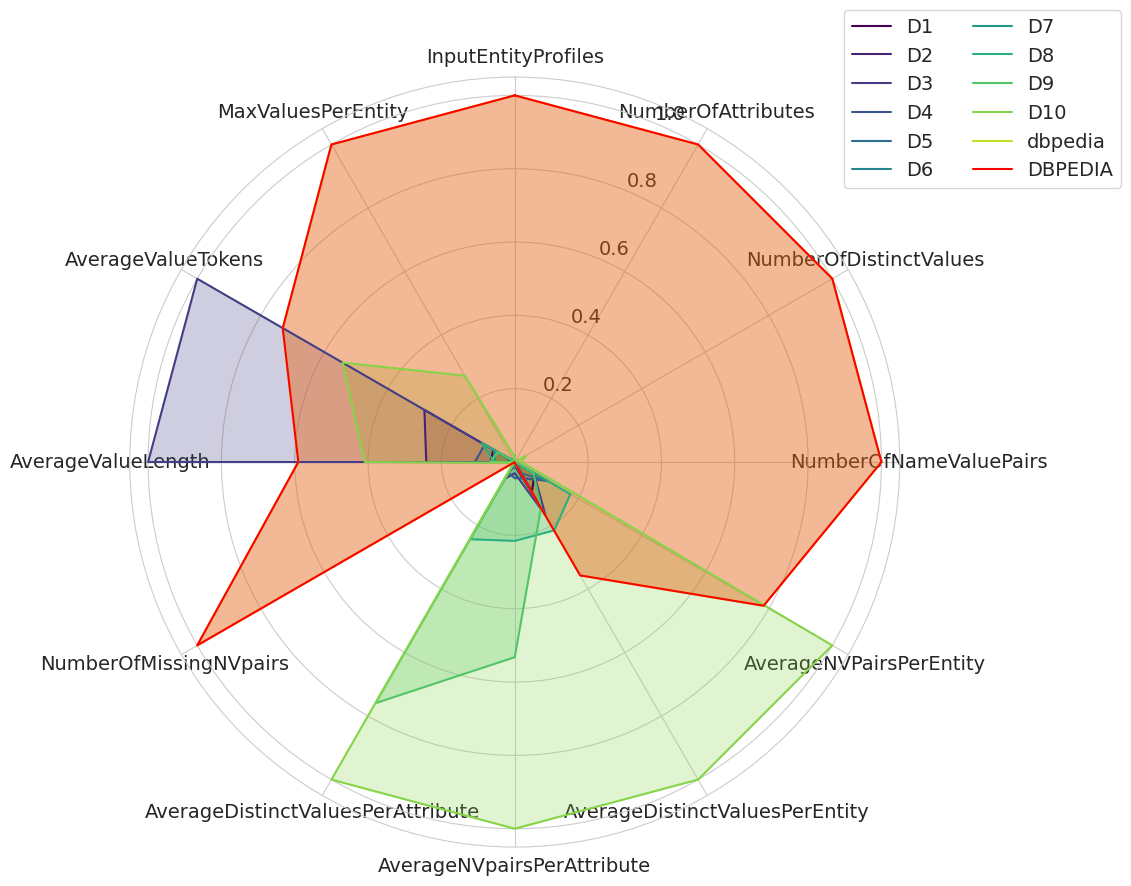
\includegraphics[width=\linewidth]{figures/predictions/dataset_specs_radar.png}
%    \caption{All dataset features comparison.}
%    \label{fig:datasets-radar}
%\end{figure}

\begin{table}[t]
\centering 
\small 
\caption{Technical characteristics of the datasets used in our experimental analysis. $|E_x|$ stands for the number of entities in data source $x$ and $|D|$ for the number of duplicates. 
} 
\label{tab:dataset-specs}
\begin{tabular}{|p{0.9cm}|p{2.1cm}|r|r|r|}
\hline
\multicolumn{1}{|c|}{\textbf{Dataset}} & \multicolumn{1}{|c|}{\textbf{Names}} & \multicolumn{1}{|c|}{\textbf{$\mathbf{|E_1|}$}} & \multicolumn{1}{|c|}{{$\mathbf{|E_2|}$}} & \multicolumn{1}{|c|}{\textbf{$\mathbf{|D|}$}} \\
\hline
\hline
\multirow{2}{*}{D1} & Restaurants1-& \multirow{2}{*}{340} & \multirow{2}{*}{2,257} & \multirow{2}{*}{89} \\
& Restaurants2 & & & \\
\hline
D2 & Abt-Buy & 1077 & 1,076 & 1,076 \\
\hline
\multirow{2}{*}{D3} & Amazon- & \multirow{2}{*}{1,355} & \multirow{2}{*}{3,040} & \multirow{2}{*}{1,103} \\
& Google Products & & & \\
\hline
D4 & DBLP-ACM & 2,617 & 2,295 & 2,225 \\
\hline
D5 & IMDB-TMDB & 5,119 & 6,057 & 1,969 \\
\hline
D6 & IMDB-TVDB & 5,119 & 7,811 & 1,073 \\
\hline
D7 & TMDB-TVDB & 6,057 & 7,811 & 1,096 \\
\hline
\multirow{2}{*}{D8} & Walmart- & \multirow{2}{*}{2,555} & \multirow{2}{*}{22,075} & \multirow{2}{*}{853} \\
& Amazon & & & \\
\hline
D9 & DBLP-Google Scholar & 2,517 & 61,354 & 2,309 \\
\hline
D10 & IMDB-DBpedia & 27,616 & 23,183 & 22,864 \\
\hline
\hline
D11 & DBpedia & 1,190,734 & 2,164,041 & 892,579 \\
\hline
\end{tabular}
\end{table}

\subsection{Experimental setup}
\label{sec:expSetup}
All experiments were implemented in Python, v. 3.9. For the implementation of the ETEER pipeline, we used pyJedAI v. 0.1.8\footnote{\underline{https://github.com/AI-team-UoA/pyJedAI}}. 
%To tackle Problem 1, 
For the implementation of the sampling algorithms, we used Optuna v. 3.6.1\footnote{\underline{https://optuna.org}}. 
%: 4381MiB / 128831MiB.
All 
%Optuna,  Linear Regression approach and
%Trials, \& DL (in general pyJedAI)
%pyJedAI 
experiments 
%for that problem 
were executed on a server running 
%executed on [OS: 
Ubuntu 22.04, 
%equipped 
with Intel Core i7-9700K @4,9GHz and 68 GB RAM.
%: 6622MiB / 64228MiB]
%D11 experiment was executed in the same server.

%\textbf{Evaluation.} The evaluation metrics include mean squared error (MSE), the ratio of the best-predicted F1-score to the \textit{global maximum F1}-score. After exploring all Optuna and Grisearch trials, the maximum F1-score per dataset, serves as the global best F1-score (GB-F1). Also, for the evaluation of the predicted configurations we measured the difference between the predicted and actual best scores. Specifically, this metric will be found later as \textit{Performance} and it is the fraction of ETEER predicted configuration F1 divided by the GB-F1 for each dataset.


\textbf{Datasets.} For Record Linkage, we use 11 publicly available, real-world datasets that are popular in the literature~\cite{DBLP:journals/pvldb/Thirumuruganathan21,DBLP:journals/pvldb/KopckeTR10,DBLP:conf/sigmod/MudgalLRDPKDAR18}. Their technical characteristics are reported in Table~\ref{tab:dataset-specs}. $D_{1}$, which was first used in OAEI 2010,
%\footnote{\underline{http://oaei.ontologymatching.org/2010}}, 
contains restaurant descriptions. $D_{2}$ encompasses duplicate products from the online retailers Abt.com and Buy.com \cite{DBLP:journals/pvldb/KopckeTR10}. $D_{3}$ matches product descriptions from Amazon.com and the Google Base data API (GB) \cite{DBLP:journals/pvldb/KopckeTR10}. $D_{4}$ entails bibliographic data from DBLP and ACM \cite{DBLP:journals/pvldb/KopckeTR10}. $D_{5}$, $D_{6}$ and $D_{7}$ involve descriptions of television shows from TheTVDB.com (TVDB) and of movies from IMDb and themoviedb.org (TMDb) \cite{DBLP:conf/esws/ObraczkaSR21}. $D_{8}$ matches product descriptions from Walmart and Amazon \cite{DBLP:conf/sigmod/MudgalLRDPKDAR18}. $D_{9}$ involves bibliographic data from publications in DBLP and Google Scholar (GS) \cite{DBLP:journals/pvldb/KopckeTR10}. Finally, 
$D_{10}$ interlinks movie descriptions from IMDb and DBpedia \cite{DBLP:journals/vldb/PapadakisETHC23}, including a different snapshot of IMDb than $D_5$~and~$D_6$. 
% Finally, D11 matches two different versions of DBpedia that chronologically differ by 3 years \cite{DBLP:journals/is/PapadakisMGSTGB20}. 

% Note that D11 is only used to address RQ3 in Section \ref{sec:expProblem2}, unlike the other datasets, which are used in all other experiments.
%Figure \ref{fig:datasets-radar} explores the dataset features extracted from each dataset, illustrating that D2 through D6 exhibit similar feature values, whereas D8, D9, D10, and particularly D11 differ significantly, with D11 representing a completely distinct feature area.

%{\color{red}Explain that D11 is used only in Problem 2 and why.}

%{\color{red} The training data was preprocessed by scaling and converting categorical variables into dummy variables to maintain consistency across all datasets. WHERE SHOULD THIS SENTENCE GO? Vasilis: mallon pouthena `h estw sto github}

\begin{table*}[t]
\begin{center}  
\small 
\caption{Performance of the two baseline methods for Problem 1: (a) the default workflow (st5, 10, UniqueMappingClustering, 0.5), and (b) the best grid-search trial. For the latter, we also report the parameter configuration.}
\label{tab:best-gridesearch-trials}
\begin{tabular}{|c||c|c||c|c|c|c||c|c|c|}
\hline
\multirow{2}{*}{Dataset} & \multicolumn{2}{c||}{Default configuration} & \multicolumn{7}{c|}{Best grid-search configuration} \\
& F1-score & Runtime (sec) & LM & K & Clustering & Threshold & F1-score & Runtime (sec) & Grid search time (hrs) \\
\hline
\hline
D1 & 47.44 & 1.90 & smpnet & 3 & CCC & 0.90 & 75.53 & 2.87 & 41 \\
D2 & 85.85 & 3.28 & st5 & 10 & UMC & 0.35 & 85.85 & 2.51 & 38 \\
D3 & 57.35 & 1.49 & sminilm & 7 & UMC & 0.45 & 59.19 & 1.43 & 45 \\
D4 & 97.56 & 4.45 & st5 & 1 & UMC & 0.80 & 98.60 & 1.43 & 45 \\
D5 & 57.74 & 5.05 & st5 & 6 & KC & 0.75 & 78.73 & 2.98 & 60 \\
D6 & 30.39 & 1.81 & sminilm & 1 & UMC & 0.55 & 60.25 & 0.91 & 71 \\
D7 & 35.68 & 2.21 & sminilm & 93 & CCC & 0.80 & 67.36 & 28.64 & 74 \\
D8 & 35.82 & 4.46 & st5 & 4 & KC & 0.90 & 47.56 & 3.19 & 145 \\
D9 & 92.04 & 13.11 & st5 & 42 & KC & 0.80 & 94.89 & 21.37 & 329 \\
D10 & 53.63 & 27.96 & st5 & 2 & KC & 0.65 & 56.12 & 28.77 & 320 \\
\hline
\end{tabular}
% \vspace{-8pt}
\end{center}  
\end{table*}

\subsection{Evaluation Results}
\label{sec:tackleProblem1}
We address three research questions while tackling Problem~1:
\begin{enumerate}[leftmargin=*, label=RQ\arabic*), start=1]
    \item Which of the sampling-based search algorithms 
    %of those discussed 
    in Section \ref{sec:problem-1} converges faster 
    %i.e., with fewer trials, 
    to its maximum performance?
    \item Does sampling-based search outperform the baselines with respect to effectiveness?
    \item Does sampling-based search outperform the baselines with respect to time efficiency?
\end{enumerate}

We use two approaches as baselines: 
\begin{enumerate}[leftmargin=*]
    \item A default configuration based on \cite{DBLP:journals/pvldb/ZeakisPSK23} that combines the s-t5 language model with $k$=10, Unique Mapping Clustering and similarity threshold = 0.5. 
    %The performance of this baseline method is reported in Table \ref{???}.
    \item The best performance estimated by grid search among the configuration parameters in Table \ref{tab:parameter-values}. %The corresponding performance is reported in Table \ref{tab:best-gridesearch-trials}.
\end{enumerate}

The performance of those baselines per dataset with respect to effectiveness and time efficiency is reported in Table~\ref{tab:best-gridesearch-trials}.

\textbf{RQ1.}
We evaluate all samplers discussed in Section~\ref{sec:problem-1}, configuring each one 
%\textit{TPESampler}, \textit{RandomSearchSampler}, \textit{QMCSampler}, and \textit{GPSampler}. Optuna was configured 
to run 100 trials per dataset, according to the recommendations from the Optuna documentation\footnote{\underline{https://optuna.readthedocs.io/en/stable/reference/samplers/index.html}}. To analyze the convergence behavior of each sampler, we vary the maximum number of trials from 5 to 100, in increments of 5. For each budget of trials, we perform experiments with five different random seeds and consider the average, thus providing a robust estimation of the actual performance per number of trials. The results appear in Figure \ref{fig:samplers-convergence-avg-f1}, with the horizontal axes corresponding to the number of trials and the vertical ones to the respective average F1-score.

%The objective was to determine the number of trials needed to find a near-optimal solution. Figure \ref{fig:samplers-convergence-avg-f1} illustrates the convergence analysis of each sampler across all datasets. The y-axis shows the average of the maximum F1-scores achieved per sampler. This "maximum" refers to the highest F1-score within each set of trials (5, 10, ..., 100), and the "average" is computed across five different random seeds, providing an average of these maximum scores. The x-axis represents the different sets of trials evaluated. 

%The number of trials in Optuna is a user-defined parameter, and Optuna will execute exactly the number of trials specified. 
For all samplers, convergence is generally observed in around 30 trials for most datasets. This means that with just 30 trials, they approximate the best performance in almost all datasets.
%μαπaccompanied by a complete ground truth. 
The only exceptions are $D_1$, $D_6$ and $D_8$. As observed in Figure \ref{fig:f1_boxplot_all}, in these datasets the portion of configuration parameters that maximize F1 is rather small. As a result, we need to increase the number of trials to much more than 30 in order to identify a configuration matching or approximating the maximum performance.

Regarding the relative performance of the considered samplers, Figure \ref{fig:samplers-convergence-avg-f1} indicates that there are no significant differences among them. Their behavior is quite similar, determined largely by the dataset at hand. Nevertheless, \textit{GPSampler} shows marginally better results in several cases.

\textbf{RQ2.} We now compare the effectiveness of the four samplers with that of the two baselines in Table \ref{tab:best-gridesearch-trials}. 
For the grid-search baseline, we also report the best-performing configuration.
%and the total time taken to run the grid search.
As expected, the default configuration consistently underperforms grid search to a significant extent. The only exception appears in $D_2$, where they yield the same F1-score, because the grid search configuration is almost identical with the default one (they differ only in the similarity threshold). Hence, for brevity, we exclusively compare the samplers with the best grid search configuration.

%To benchmark the Optuna approach, we also conducted an exhaustive grid search for each dataset. The search space explored is detailed in Table \ref{tab:parameter-values}, where the Cartesian product of all parameters results in a total of $7 \times 3 \times 19 \times 100 = 39,900$ possible configurations. 
%\comments{giati to leme edw? pws sundeetai me tin panw paragrafo? giati xreiazetai na to kseroume? mia protasi akoma xreiazetai.}

%\begin{figure*}[h!]
%    \centering
%    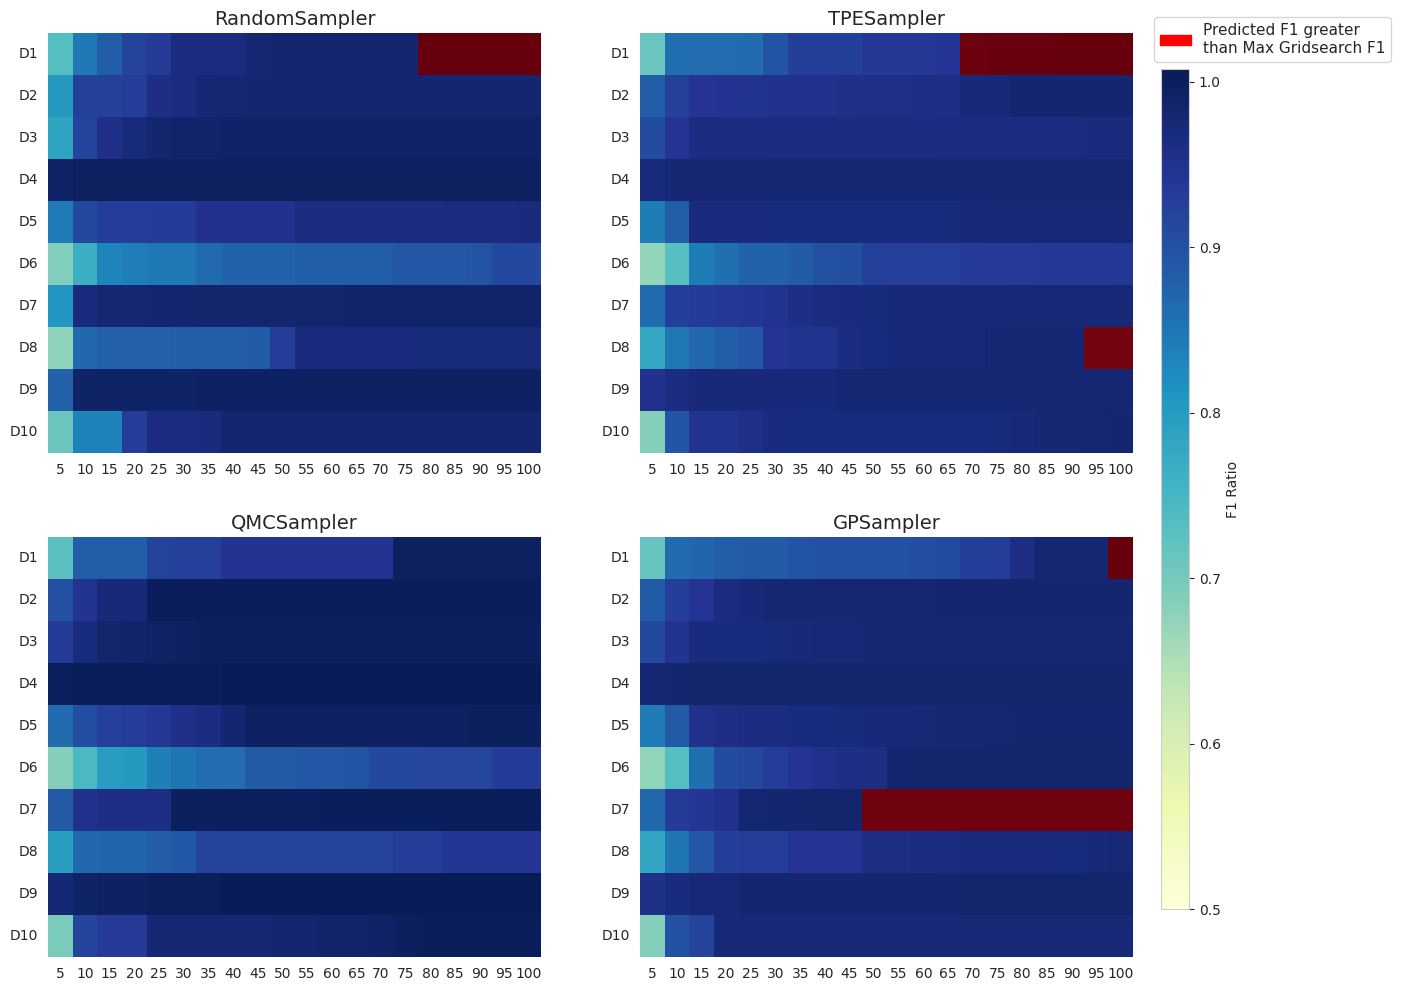
\includegraphics[width=0.97\textwidth]{Nikoletos-paper/figures/predictions/sampler_heatmaps.png}
%    \caption{Samplers F1-Ratio heatmaps.}
%    \label{fig:samplers-heatmaps-f1}
%\end{figure*}

% \begin{figure*}[t]
%     \centering
%     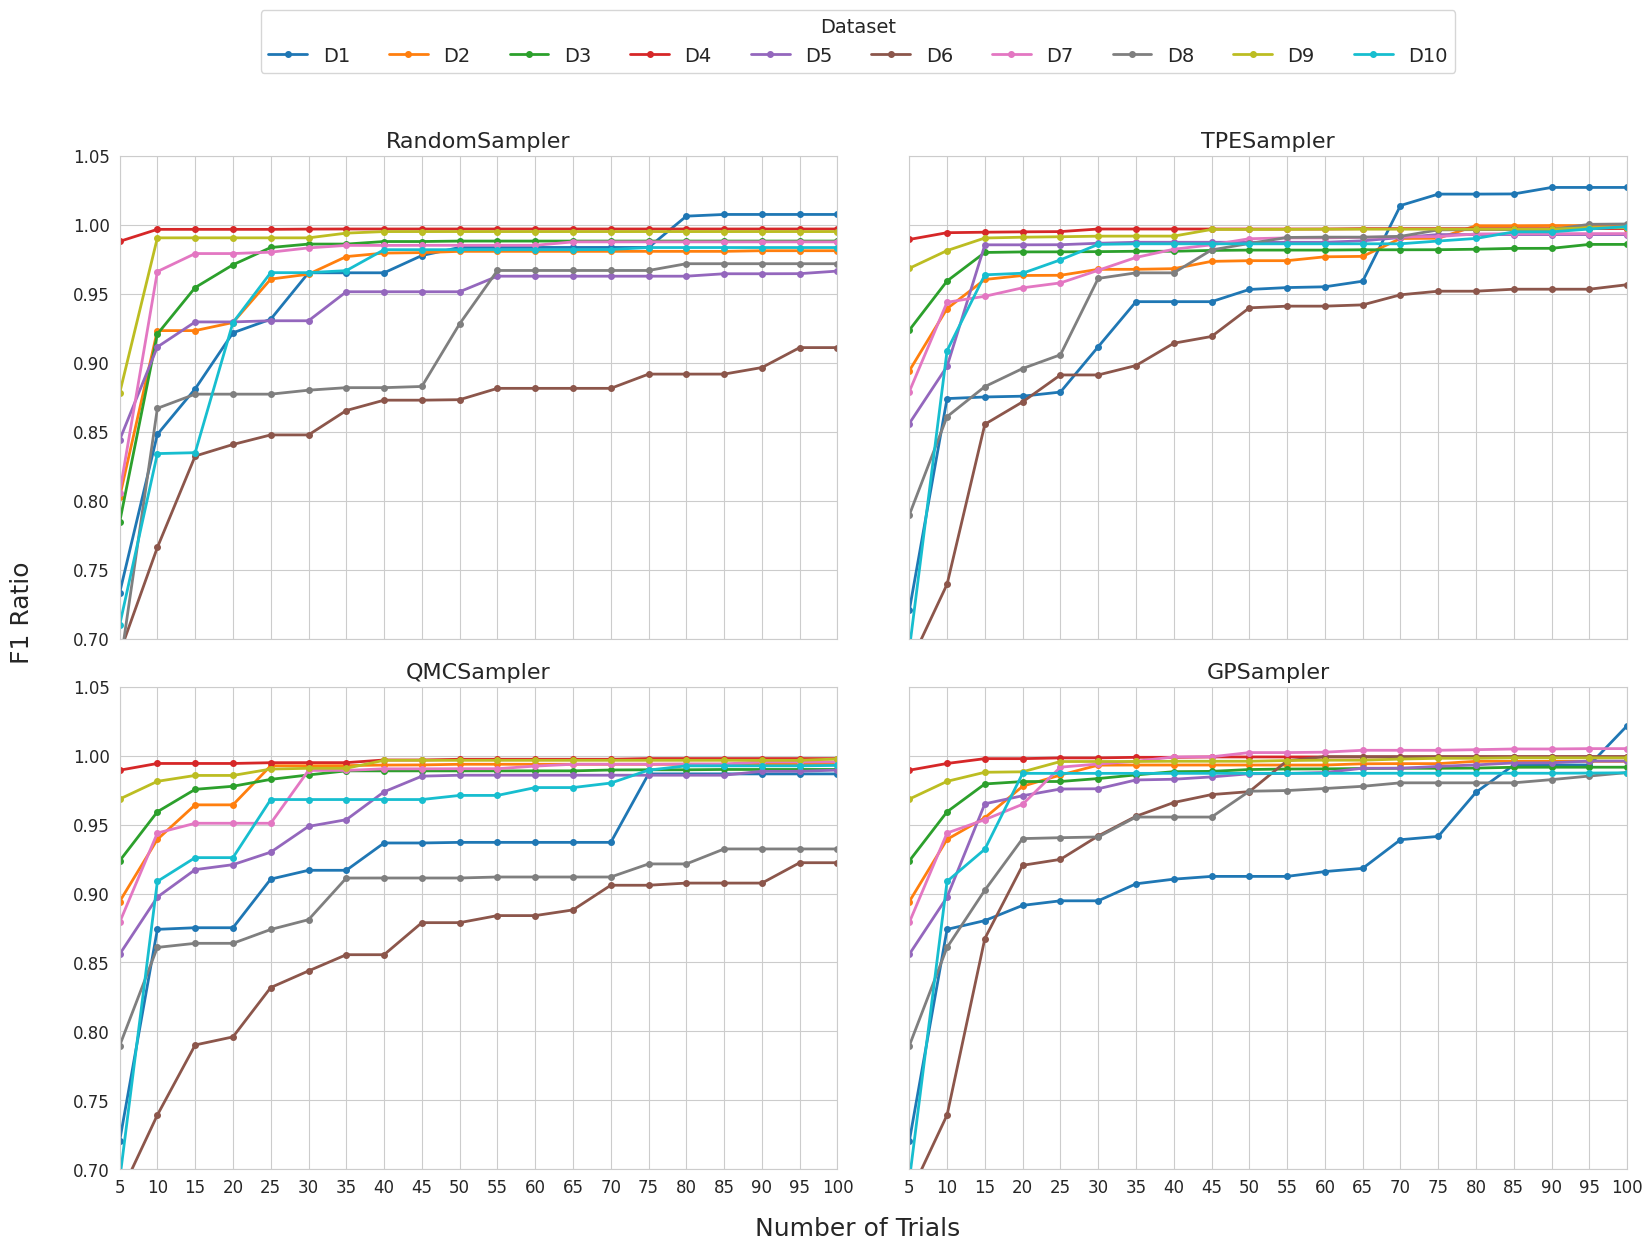
\includegraphics[width=0.8\textwidth]{Nikoletos-paper/figures/predictions/f1_ratio_vs_trials_subplots.png}
%     \vspace{-10pt}
%     \caption{The ratio between the F1-score of the sampling-based search algorithms and the F1-score of grid search.}
%     \label{fig:p1-samplers-performance-f1}
%     %\vspace{-10pt}
% %\end{figure*}

% %\begin{figure*}[t]
%     \centering
%     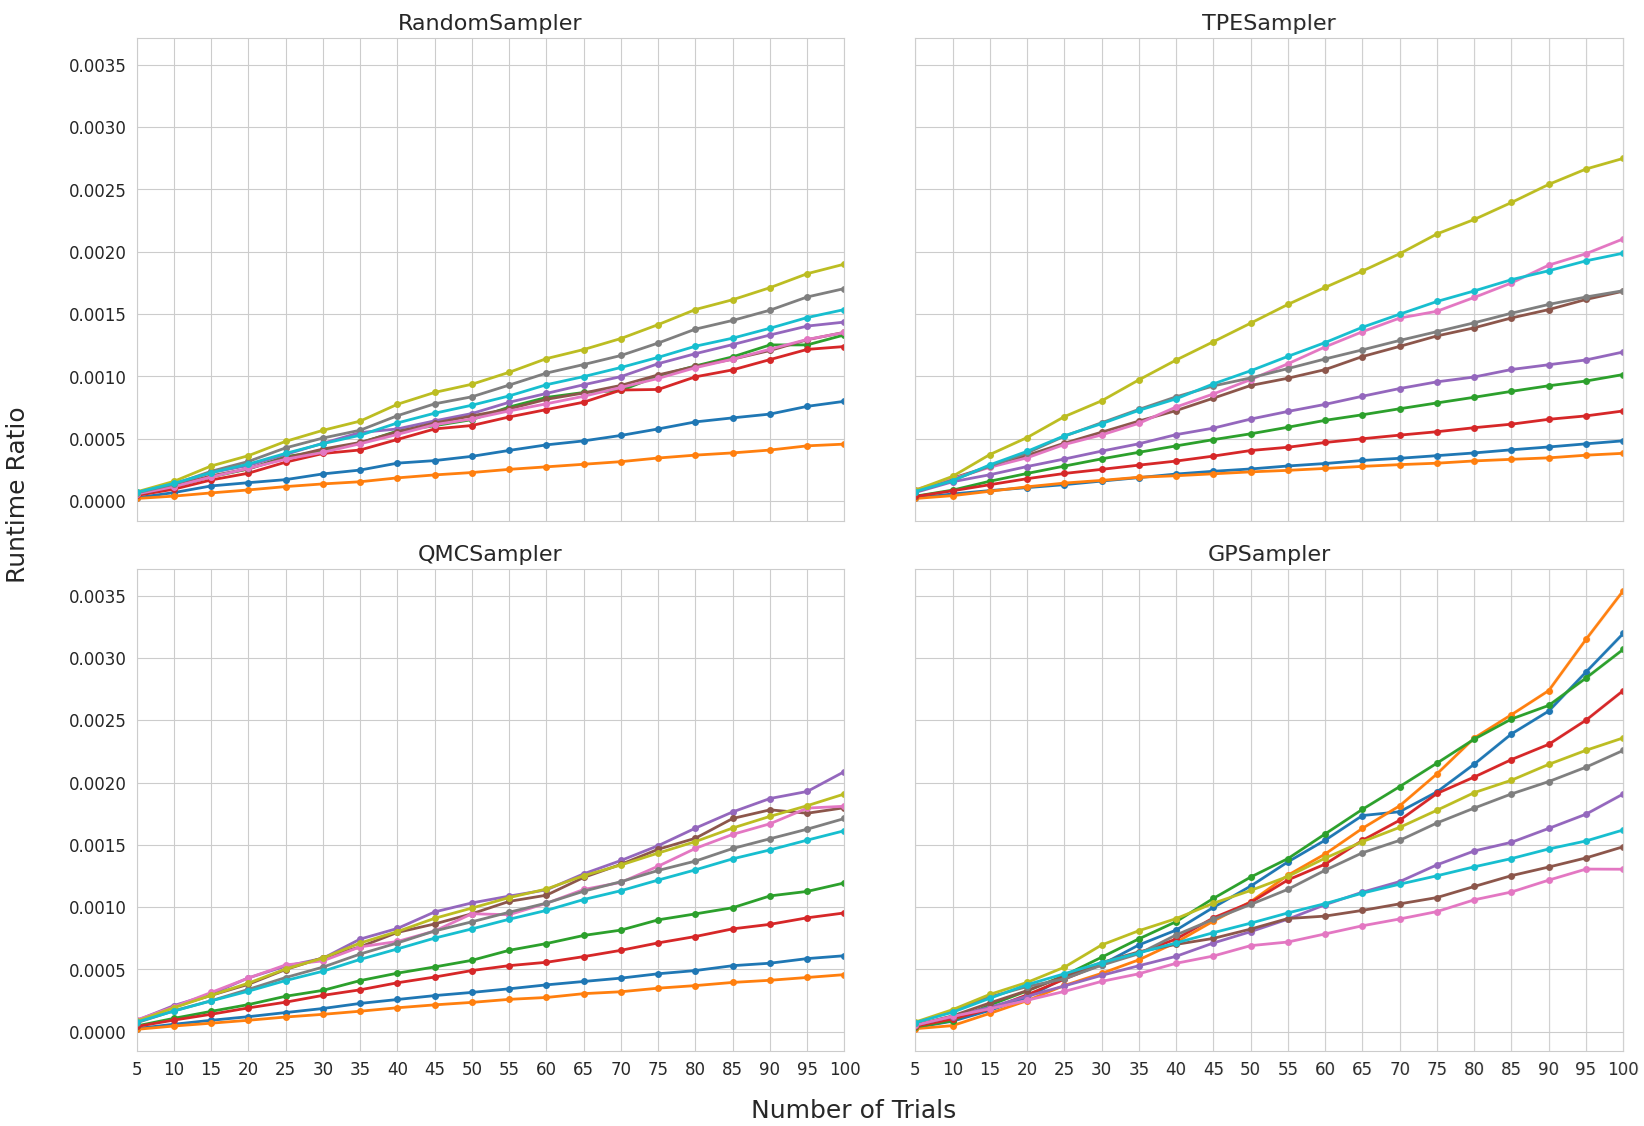
\includegraphics[width=0.8\textwidth]{Nikoletos-paper/figures/predictions/runtimes_ratio_vs_trials_subplotsV2.png}
%     \vspace{-10pt}
%     \caption{The ratio between the run-time of the sampling-based search algorithms and the run-time of grid search.}
%     \label{fig:p1-samplers-performance-runtimes}
%     \vspace{-10pt}
% \end{figure*}

\begin{figure*}[t]
    \centering
    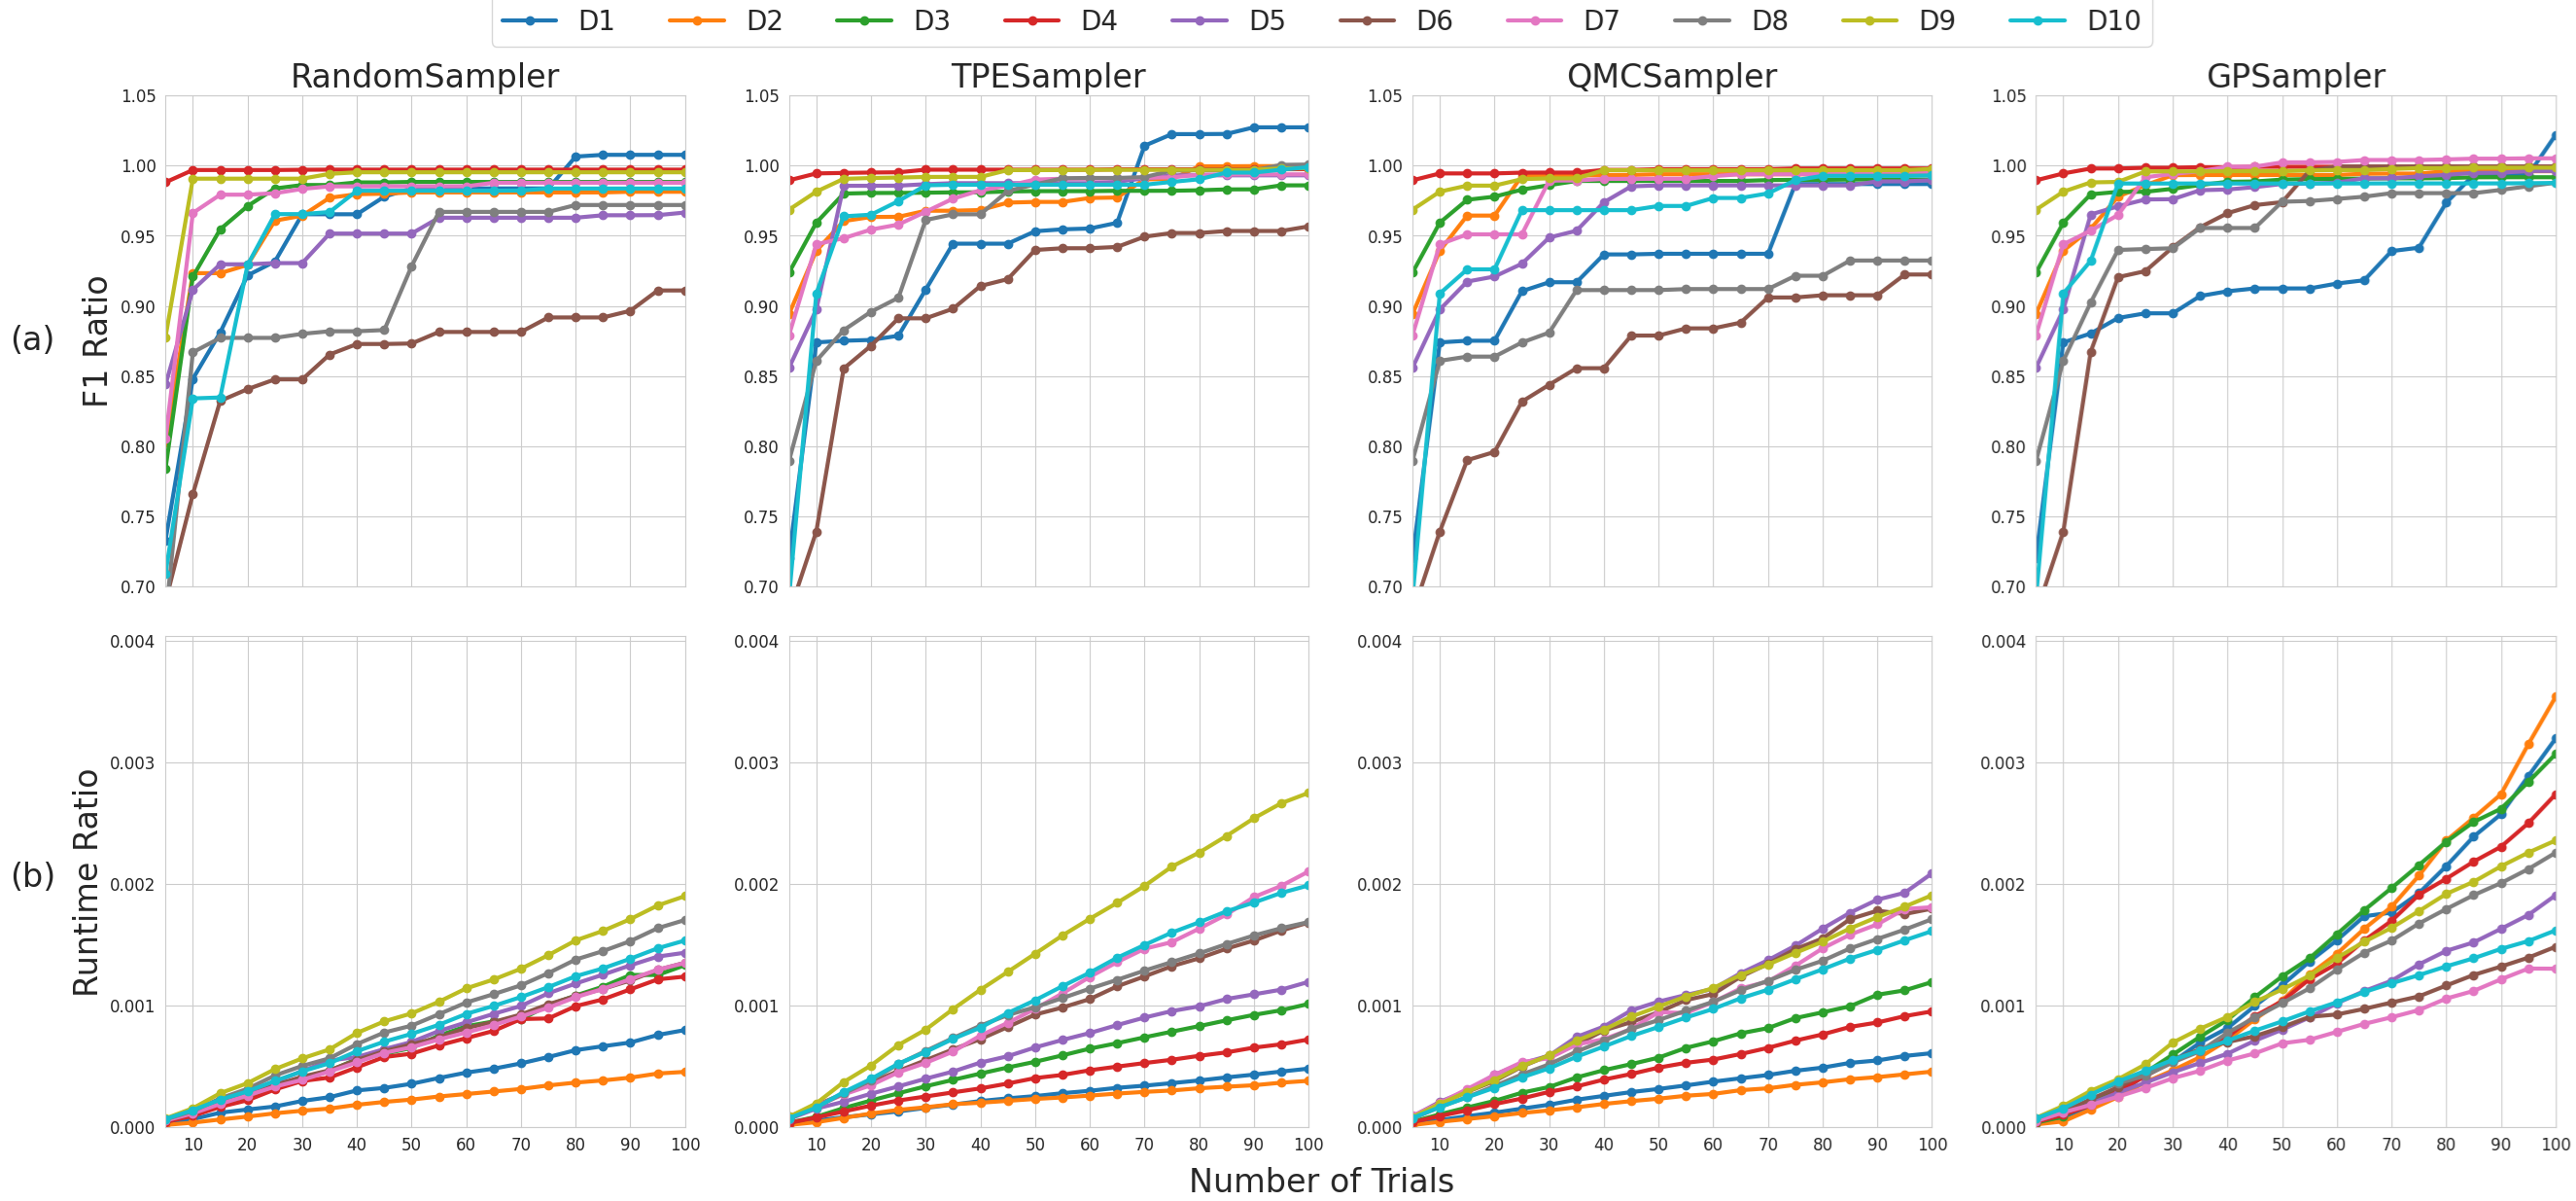
\includegraphics[width=0.99\textwidth]{Nikoletos-paper/figures/predictions/combined_f1_runtime_ratios_vs_trials.png}
    % \vspace{-10pt}
    \caption{The ratio between (a) the F1-score of sampling-based search algorithms and grid search, and (b) their run-times.
    %algorithms and the F1-score/Runtime of grid search.
    }
    \label{fig:p1-samplers-performance-f1}
\end{figure*}

This comparison is depicted in Figure \ref{fig:p1-samplers-performance-f1}(a), which contains a separate diagram for each sampler with its convergence to the best grid search performance in Table \ref{tab:best-gridesearch-trials}. The vertical axes 
%in Figure \ref{fig:p1-samplers-performance-f1} 
correspond to \textit{F1 ratio}, which is defined as ``samplerF1''/``gridSearchF1''. That is, an F1 ratio of 1.0 indicates that the two approaches yield the same F-Measure despite their different configuration. Values lower than 1.0 indicate lower sampling-based performance than grid search, while ratios $>1.0$ denote that the sampler identified a configuration that outperforms all those tested by grid search. This should be attributed to the discrete similarity thresholds considered by grid search, unlike samplers, which may consider any value in $[0,1]$.

%We observe that the 
RandomSampler underperforms grid search in almost all cases. Yet, with just 20 trials, its F1 ratio exceeds 0.90 in all datasets but
%is less than 10\% lower than the best one of grid search, except for 
$D_1$, $D_6$ and $D_8$.
These three datasets 
convey very few top-performing configurations, as shown in Figure \ref{fig:f1_boxplot_all}. 
%RandomSampler 
%reaches 95\% of grid search's F1 
Note also that with just 30 trials, its F1 ratio exceeds 0.95 in all datasets but $D_1$, $D_6$ and $D_8$. In $D_1$, RandomSampler converges to grid search after 70 trials, outperforming it to a minor extent after 80 trials, while in $D_6$ and $D_8$, its F1 ratio raises up to 0.93 after 100 trials, because there is an even lower portion of top-performing configurations. 

TPESampler exhibits a much 
%better 
quicker
convergence. With only 20 trials, its F1 ratio is higher than 0.95 in all datasets but the most challenging ones, namely $D_1$, $D_6$ and $D_8$. For 30 trials, its F1 ratio is lower than 0.95 only in two datasets: $D_1$ and $D_6$. In $D_1$, TPESampler outperforms grid search by $\sim$2.5\% after just 65 trials, while in $D_6$, its F1 ratio exceeds 0.95 after 70 trials. 

QMCSampler exhibits a performance similar to RandomSampler. After 20 trials, its F1 ratio is lower than 0.90 in only two datasets: $D_6$ and $D_8$. After 30 trials, its F1 ratio is lower than 0.95 in three datasets: $D_5$, $D_6$ and $D_8$. For the first two of these datasets, it matches the effectiveness of grid search after 55 trials, but its F1-score in $D_8$ is almost 9\% lower than grid search after 100 trials. In $D_1$, QMCSampler converges faster than all other samplers, with its F1 ratio exceeding 0.95 after 30 trials and 1.00 
%while outperforms grid search 
after 80 trials. 

Finally, GPSampler is similar to TPESampler. After 20 trials, its F1 ratio exceeds 0.95 in all but the three most challenging datasets, i.e., $D_1$, $D_6$ and $D_8$. For the last two, the F1 ratio raises to 0.94 after 30 trials, with $D_1$ converging much slower, after 80 trials, eventually outperforming grid search after 100 trials. The same applies to a minor extent to $D_7$, too. Note also that GPSampler is the only approach that matches or exceeds the performance of grid search across all datasets after 100 trials. Hence, it is considered the top performing approach, albeit to a minor extent in most cases.

\begin{table}[t]
\centering
\small 
\setlength{\tabcolsep}{2.5pt}
\caption{The highest F1-score among the configurations considered by the sampling-based search algorithms in Section~\ref{sec:problem-1}.}
\label{tab:global-bestf1s}
\begin{tabular}{|c|c|c|c|c|c|c|r|}
\hline
Dat. & LM & k & Clustering & Threshold & Sampler & F1 & RT (s) \\
\hline
\hline
D1 & st5 & 73 & CCC & 0.874280 & tpe & 78.43 & 0.95 \\
D2 & st5 & 10 & UMC & 0.594537 & tpe & 85.85 & 0.38 \\
D3 & sminilm & 10 & UMC & 0.429178 & random & 58.97 & 0.43 \\
D4 & st5 & 1 & UMC & 0.759879 & gps & 98.56 & 6.58 \\
D5 & st5 & 1 & CCC & 0.765179 & gps & 78.92 & 3.67 \\
D6 & sminilm & 1 & UMC & 0.555229 & gps & 60.42 & 1.30 \\
D7 & sminilm & 84 & CCC & 0.811881 & gps & 67.76 & 5.22 \\
D8 & st5 & 75 & KC & 0.920773 & tpe & 49.53 & 6.45 \\
D9 & st5 & 65 & KC & 0.830563 & tpe & 94.92 & 16.83 \\
D10 & st5 & 2 & KC & 0.269090 & tpe & 56.11 & 14.03 \\
\hline
\end{tabular}
\end{table}


\textbf{RQ3.} To estimate the relative time efficiency of grid and sampling-based search, we define the \textit{runtime ratio} as $rt(sa, n)/rt(gs)$, where $rt(sa, n)$ stands for the overall run-time required by each sampler for $n$ trials, on average, across the 5 iterations (based on different seeds), and $rt(gs)$ for the overall run-time required by grid-search for the same dataset, as reported in Table \ref{tab:best-gridesearch-trials} -- $rt(sa, n)$ and $rt(gs)$ involve both the time required for generating the next parameter configuration to be tested and the run-time of the corresponding ETEER pipeline. The runtime ratio is defined in $[0,1]$, with values $<1$ indicating 
%higher time efficiency, i.e.,
that sampling-based is faster than grid search. 

The actual values of the runtime ratio per sampler, dataset and number of trials is depicted in Figure \ref{fig:p1-samplers-performance-f1}(b). We observe that in all cases, its value is well below 0.35\%. This means sampling-based search is consistently faster than grid search by more than 285 times. Typically, the larger a dataset is, the higher is the runtime ratio, because of the more time-consuming ETEER pipelines that have to be evaluated. The relative run-time of the sampling-based algorithms is determined by their relative time complexity: the fastest approach is RandomSampler followed in close distance by QMCSampler, given their time complexity, $O(d)$ and $O(d n)$, resp.; TPESampler is consistently slower, $O(d n logn)$, with GPSampler exhibiting the highest run-times, due to its cubic time complexity.

\begin{figure}[t]
    \centering
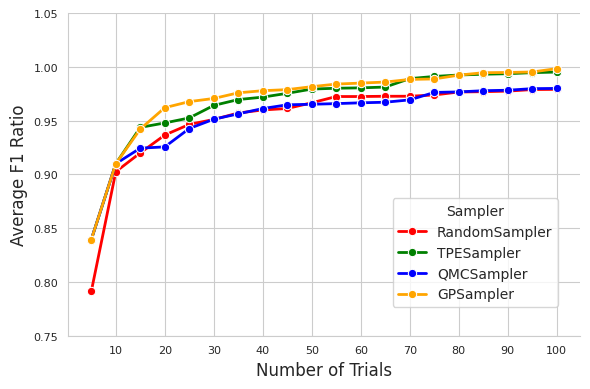
\includegraphics[width=0.97\linewidth]{Nikoletos-paper/figures/predictions/average_f1_ratios_across_datasets.png}
    % \vspace{-10pt}
    \caption{Average F1 score per sampler and per trial, across all the datasets.}
    \label{fig:mean-F1-samplers-performance-f1}
\end{figure}

\textbf{Conclusions.} We can conclude that all considered sampling-based search algorithms for parameter fine-tuning are capable of approximating the performance of grid search in any of the considered datasets, while being faster by at least 2 orders of magnitude.
%despite using 399 times less trials. 
The larger the portion of top-performing configurations in a dataset, the fewer trials are needed by these algorithms. Nevertheless, they consistently underperform grid search, albeit to an insignificant extent ($\ll0.5\%$).
%Note, though, that they rarely outperform grid search: 
Comparing their best performance in Table~\ref{tab:global-bestf1s} with the best grid search one in Table~\ref{tab:best-gridesearch-trials}, we observe that only in $D_1$ and $D_8$ the former outperforms the latter by 2\%-3\%. {Overall, though, the difference between the two approaches is statistically insignificant ($p=0.13437$) (unlike the difference between the default configuration in Table~\ref{tab:best-gridesearch-trials} and the best sampling performance in Table~\ref{tab:global-bestf1s}).}
%-- in all other cases, their difference is statistically insignificant . 
As a result, sampling-based search basically 
%thus offering a much faster approach to approximating grid search.
%Overall, we can conclude that the sampling-based algorithms for parameter fine-tuning 
offers a much better balance between effectiveness and time efficiency than grid search: for the same F1 score, the number of trials and the corresponding run-time is reduced by 2 or even 3 orders of magnitude. Among the sampling-based algorithms, the fastest convergence and the highest effectiveness typically correspond to GPSampler, especially for 20-30 trials, as shown in Figure \ref{fig:mean-F1-samplers-performance-f1}, which estimates the average F1 per number of trials for each sampler across all datasets in Table~\ref{tab:dataset-specs}. {Note that the superiority of GPSampler over the other three samplers is statistically significant ($p\ll0.05$) in Figure~\ref{fig:mean-F1-samplers-performance-f1}}.


\section{Tackling Problem 2}
\label{sec:problem-2}

\begin{figure*}[t]
    \centering
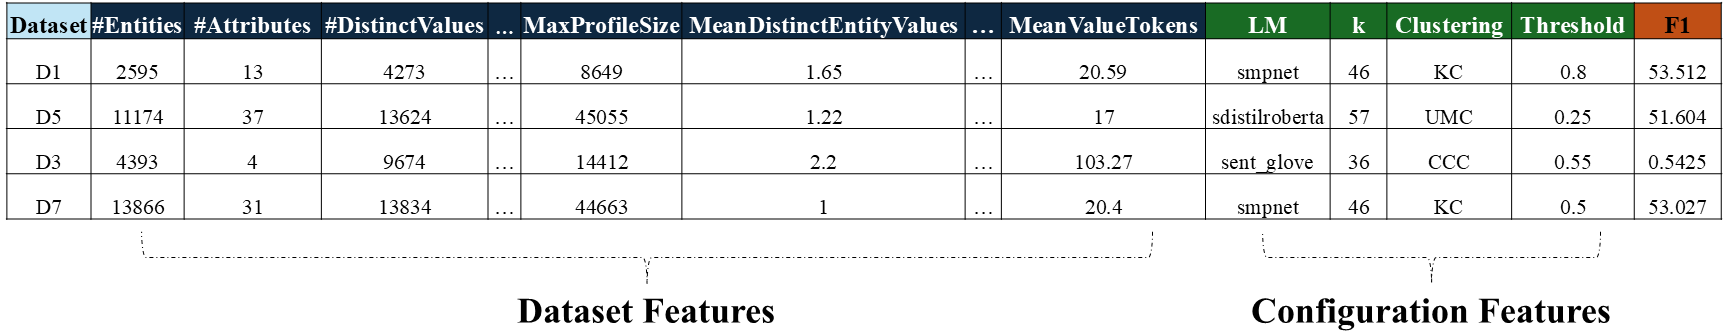
\includegraphics[width=0.95\linewidth]{figures/dataset/join_dataset_trials.png}
    \caption{The feature vector of the regression model addressing Problem \ref{pr:pr2}. It combines 12 dataset features with 4 configuration parameters of the ETEER pipeline in Figure \ref{fig:eeter_pipeline}. Note that the leftmost column ("Dataset") is only added for clarification  purposes.}
    \label{fig:join_dataset_trials}
\end{figure*}

To address Problem \ref{pr:pr2}, we define a regression model that treats every combination of a dataset $D$ and a set of configuration values $V$ as an instance. For the labelled instances, the dependent variable corresponds to the F1 score of the ETEER pipeline in Figure \ref{fig:eeter_pipeline}, configured with $V$, when applied on $D$. For the unlabelled instances, the goal is to predict this F1 score. 

To put this approach into practice, we need to define the following aspects of the regression model:

\begin{itemize}[leftmargin=*]
    \item Feature engineering. This means that we need to define the feature vector that is fed to the regression model during the training and prediction phases. This vector consists of two types of dimensions: (i) \textit{dataset features}, and (ii) \textit{configuration features}. For the former, which capture the characteristics of a Record Linkage dataset, we consider features from dataset profiles defined in the literature, as explained in Section \ref{sec:datasetProfiling}. For the configuration features, the definition is straightforward: there is a separate feature for each parameter of the ETEER pipeline in Table \ref{tab:parameter-values}. The domain of each feature is the same as the respective numeric parameter, in the case of $k$ and the similarity threshold. The categorical parameters (i.e., LM and clustering algorithm) are transformed into a binary format through one-hot encoding. 
    \item Instance generation. We define three approaches for generating the labelled instances that will be used for training the regression model: (i) grid search, (ii) sampling-based search, and (iii) their combination. The resulting configuration features are combined with the dataset features extracted from the datasets D1-D10 in Table \ref{tab:dataset-specs} except for the one that should be fine-tuned. For each feature vector, we apply the respective parameter configuration to a particular dataset with known ground truth in order to estimate the corresponding target variable, i.e., the F1-score. 
    \item Learning process. We use two methods for training the regression model: (i) Random Forest and (ii) AutoML. A critical characteristic is that both methods incorporate feature selection, which is necessary due to the high dimensionality of the feature vector defined by feature engineering and the unclear contribution of each dimension. Another crucial characteristic is that they both achieve very high performance under versatile settings \cite{DBLP:journals/csur/KarmakerHSXZV22,DBLP:journals/bioinformatics/NguyenJGSALJCGM21}.
\end{itemize}

%{\color{red}As explained above, the sampling algorithms are guided by the performance that corresponds to each tested configuration. In the context of Problem 2, though, this approach is inapplicable, due to the lack of a ground truth for the dataset at hand. Nevertheless, ETEER fine-tuning can still be modelled as a learning-based task by leveraging the ground truths from other datasets.

%When no ground truth file is provided, a pyJedAI user does not have the ability to use the methodology described earlier \comments{[why?]}. Also, configurations must be data sensitive, meaning that we need to extract some generic features from the given dataset. \comments{explain more the features extracted?}
%\comments{Here, we describe what we CANNOT do, but we should describe also what we actually do.}

%\begin{table}[t]
{\footnotesize
\begin{center}  
\label{tab:featureSet}
\begin{tabular}{|p{2cm}|p{5cm}|}\hline
\textbf{Dataset Feature} & \textbf{Definition} \\
\hline
Number of entities & The total number of entities in the dataset \\ \hline
Number of attributes & The total number of attributes for the entities \\ \hline
Number of distinct values & The total number of distinct values across all attributes \\ \hline
Number of name-value pairs & The total number of name-value pairs in the dataset \\ \hline
Mean name-value pairs per entity & The average number of name-value pairs per entity \\ \hline
Mean name-value pairs per attribute & The average number of name-value pairs per attribute \\ \hline
Number of missing name-value pairs & The total number of missing name-value pairs in the dataset \\ \hline
Mean distinct values per attribute & The average number of distinct values per attribute \\ \hline
Mean total attribute value length per entity & The average total length of attribute values per entity \\ \hline
Mean attribute value tokens per entity & The average number of tokens in attribute values per entity \\ \hline
Mean distinct values per entity & The average number of distinct values per entity \\ \hline
Max values per entity & The maximum number of values for any single entity \\ \hline
\end{tabular}
\caption{The list of dataset features.}
\end{center}  
}
\end{table}

%\subsection{Building a model over trials}

%The previous experimental methodology involved multiple runs of different executions on ten distinct datasets \comments{what datasets?}, resulting in a comprehensive trials dataset. In this new approach, the trials and configurations serve as our primary data. 
%More specifically, we frame our solution to Problem 2 as a regression task that is addressed in the following way: 
%\begin{enumerate}[leftmargin=*]
%    \item Dataset profiling: We define a set of features that capture the characteristics of a Record Linkage dataset.
%    \item Definition of independent variables: The \textit{dataset features} defined in the previous step are concatenated with four \textit{configuration features}, which stand for the four configuration parameters of the ETEER pipeline in Figure \ref{fig:eeter_pipeline}. This means that each feature vector combines parameter configurations with general characteristics of a particular dataset.
%    \item Estimation of dependent variables: For each feature vector, we apply the respective parameter configuration to a particular dataset with known ground truth in order to estimate the corresponding target variable, i.e., the corresponding F1-score. Applying numerous ETEER configurations to multiple datasets with known ground truth yields a sizeable training set.
%    \item Model training: A regression algorithm is trained on the labelled instances generated by the previous steps.
%    \item Prediction phase: The learned model is applied to the feature vectors extracted from the given dataset $D$ through grid search. Note that there is a different feature vector for each parameter configuration we want to try, while dataset $D$ lacks any ground truth. The feature vector yielding the highest predicted F1-score 
    %(\comments{mipws F1-score opws to exeis sto section 2?}) 
    %is selected as the optimal configuration for dataset $D$.
%\end{enumerate}
%To put this idea into practice, we need to implement the following:
%\begin{enumerate}[leftmargin=*]
%    \item Dataset Profiling: define the dataset features capturing general characteristics of an ER dataset,
%    \item Instance Generation: define the approach for generating the configuration values to be tested.
%\item Choose the datasets with known ground truth that will generate the training instances.
%    \item Learning process: define the method used for training a performance prediction model.
%\end{enumerate}
%For Point (3), we choose a set of 11 established datasets for Record Linkage that are publicly available and widely used in the literature, while encompassing a complete ground truth. See Section \ref{sec:experiments} for more details. We delve into Points (1), (2) and (4) in the following.
%}

We delve into each of these three steps in the following.

\subsection{Feature Engineering}
\label{sec:datasetProfiling}

The dataset features used by our approach should adhere to the following principles: 
\begin{enumerate}[leftmargin=*]
    \item They should be \textit{generic}, applying seamlessly to any ER dataset, regardless of its format (i.e., be it structured like a CSV file or semi-structured like JSON file or RDF dump) and regardless of the corresponding flavor of ER (i.e., Record Linkage, Deduplication or Multi-source ER).
    \item They should be \textit{effective}, capturing all aspects of given dataset $D$ that might affect the performance of an ETEER pipeline on~$D$.
    \item They should be \textit{efficient}, involving low extraction cost and overhead, so that it is possible to extract predictions for numerous feature vectors from the learned model.
\end{enumerate}

In this context, we consider the following wide range of dataset features, which captures the main ones proposed in the literature. Our goal is to perform feature selection during the learning process so as to identify the top performing features for the task at hand.
\begin{enumerate}[leftmargin=*, label=F\arabic*), start=1]
    \item \#Entities \cite{DBLP:conf/sigmod/IlyasMHBA04}: the total number of entities in the dataset, i.e., $|\mathcal{E}_1| + |\mathcal{E}_2|$ in the case of Record Linkage datasets. This feature 
    %is an indication of the size of the dataset, which 
    affects proportionately the number of nearest neighbors returned for each query entity.
    \item \#Attributes: The total number of distinct attributes describing all given entities in $\mathcal{E}_1$ and $\mathcal{E}_2$. This is an indication of the schema heterogeneity of the given dataset(s), with higher values indicating more heterogeneous and noisy datasets. This is called schema complexity in~\cite{DBLP:conf/cikm/PrimpeliB20}.
    \item \#DistinctValues \cite{DBLP:conf/sigmod/IlyasMHBA04}: the total number of distinct values across all attributes. Higher values suggest a larger diversity in the description of entity profiles, which indicates more challenging settings for an ETEER pipeline.
    \item \#AttributeValuePairs: the total number of attribute-value pairs in all entity profiles of the given dataset(s). Higher values indicate larger profile sizes, which are probably harder to match.
    \item MeanProfileSize: the average number of attribute-value pairs per entity, i.e., F4/F1. The rationale is the same as~F4.
    %\comments{mipws attribute-value pairs? epeidi sto 2 kai 3 les attributes}
    \item MeanAttributeSize: the average number of name-value pairs per attribute, i.e., F4/F2. Higher values indicate attributes with a larger domain, thus diversifying the entity descriptions and rendering ER a more challenging~task.
    \item MeanDistinctEntityValues: the average number of distinct values per entity, i.e., F3/F1. Lower values indicate profiles with insufficient or repeated information, thus hampering ER.
    \item MeanDistinctAttributeValues~\cite{DBLP:journals/pvldb/SuchanekAS11}: the average number of distinct values per attribute, i.e., F3/F2. Low values indicate datasets with non-distinctive attribute-value pairs, which are thus harder to deduplicate.
    \item MaxProfileSize: the maximum number of attribute-value pairs in any of the given entities. Higher values indicate harder entity matching settings, e.g., datasets with oversized profiles, which are probably associated with irrelevant and, thus, noisy values. 
    \item MissingInformation: The total number of missing attribute-value pairs in the given dataset(s), which is estimated as F1 $\times$ F7 - F4. Higher values indicate higher levels of noise in the given datasets, which hamper ER. This is called sparsity in~\cite{DBLP:conf/cikm/PrimpeliB20}.
    \item MeanValueTokens: The average number of tokens in all attribute values per entity. Lower values correspond to datasets with small entity descriptions, which probably lack sufficient information for ER. This is called textuality in~\cite{DBLP:conf/cikm/PrimpeliB20}.
    \item MeanValueLength: This is a variation of MeanValueTokens (or textuality \cite{DBLP:conf/cikm/PrimpeliB20}). It concatenates all attribute values per entity in a sentence, but instead of counting the words formed by tokenizing it on whitespace, it measures its length in characters. This length is averaged, across all input entities. Longer values indicate richer entity profiles, which might involve more distinguishing information, facilitating their deduplication.
\end{enumerate}

Note that all dataset features satisfy the requirements defined above, being generic, effective and efficient. They are concatenated with the four configuration features of the ETEER pipeline in Figure~\ref{fig:eeter_pipeline}, forming the 16-dimensional feature vector in Figure~\ref{fig:join_dataset_trials}.


\subsection{Instance Generation}
\label{sec:instanceGeneration}

%given a dataset, we extract a set of features and predict the optimal configuration. This is achieved by training a model based on configuration values and dataset features, with the goal of predicting the F1 score. The top-1 configuration, which has the maximum predicted F1 score, is then proposed as the optimal configuration. Three different approaches \comments{[which are..?]} were tested to ensure the best results and model generalization. 

We follow three different procedures for generating a set of labelled instances from every dataset:
\begin{enumerate}[leftmargin=*]
    \item \textit{Grid search} applies all configurations in Table \ref{tab:parameter-values} to estimate the dependent variable per instance, i.e., the respective F1-score.
    \item \textit{Sampling-based search} applies the four sampling methods in Section \ref{sec:problem-1} for a specific number of trials. F1-score is only estimated for these trials, yielding an equal number of labelled instances.
    \item \textit{All} merges the instances generated by the two approaches.
    %grid and sampling-based search.
\end{enumerate}

%Grid search is expected to yield a larger number of instances than sampling-based search, because the latter is bounded by the limited budget of trials. 
In all cases, we exclude instances with a zero F1 as well as duplicate instances, which have the same configuration (e.g., proposed by different samplers).
%rials, where samplers proposed configurations already covered by the grid search, were also removed from the training sets. 
Note that instance generation is a time-consuming process, due to the large number of ETEER pipelines that are evaluated. However, it constitutes an offline process that is carried out only once and, thus, does not affect the prediction time when applying the trained regression model on a new dataset that lacks a ground truth.
%for our approach when it is applied to a new dataset. %{\color{red}Nevertheless, we experimentally evaluate not only the effectiveness but also the time efficiency of this step in Section \ref{sec:expProblem2}. ISWS TO VGALOUME AUTO. DEN KSERW AN EXEI NOIMA. VASILIS: SYMFWNW


%Among these methods, grid search is expected to involve a much more time-consuming process, due to the larger number of configurations that it typically considers. However, the actual run-time of the configurations tested by grid search might be much lower than that of the configurations proposed by sampling-based search. Most importantly, instance generation is an offline process that does not affect the prediction time for the learned model. Therefore, we are mostly interested in the effectiveness of the models learned by each instance generation approach. This is experimentally assessed in Section \ref{sec:experiments}. 

\subsection{Learning process}
\label{sec:learningProcess}

%\begin{table}[ht]
\centering
\caption{Parameters Tested for RF Regression Method.}
\label{tab:regressor_params}
\begin{tabular}{|p{1.5cm}|l|l|}
\hline
\textbf{Regressor}          & \textbf{Parameter}        & \textbf{Search Space}                           \\ \hline
% \multirow{1}{*}{Lasso}      & alpha                     & \text{LogUniform}($10^{-4}$, $10^1$)                           \\ \hline
% \multirow{1}{*}{Ridge}      & alpha                     & \text{LogUniform}($10^{-4}$, $10^1$)                           \\ \hline
% \multirow{1}{*}{LR} & -                 & -                                               \\ \hline
% \multirow{8}{*}{XGBR} & n\_estimators    & $\{100,...,1000\} \subseteq \mathbb{Z}$                                   \\ \cline{2-3}
%                             & max\_depth                 & $\{3,...,10\} \subseteq \mathbb{Z}$                                      \\ \cline{2-3}
%                             & learning\_rate             & \text{LogUniform}($10^{-3}$, $10^{-1}$)                          \\ \cline{2-3}
%                             & subsample                 & \text{Uniform}($0.5$, $1.0$)                                                \\ \cline{2-3}
%                             & colsample\_bytree          & \text{Uniform}($0.5$, $1.0$)                               \\ \cline{2-3}
%                             & gamma                     & $\{0,...,5\} \subseteq \mathbb{Z}$                                        \\ \cline{2-3}
%                             & reg\_alpha                 & \text{LogUniform}($10^{-2}$, $10^{2}$)                              \\ \cline{2-3}
%                             & reg\_lambda                & \text{LogUniform}($10^{-2}$, $10^{2}$)                              \\ \hline
\multirow{5}{*}{RFR} & n\_estimators & $\{100, ..., 1000\} \subseteq \mathbb{Z}$                                  \\ \cline{2-3}
                            & max\_depth                 &  $\{3,...,10\} \subseteq \mathbb{Z}$                                      \\ \cline{2-3}
                            & min\_samples\_split         &  $\{2,...,20\} \subseteq \mathbb{Z}$                                      \\ \cline{2-3}
                            & min\_samples\_leaf          &  $\{1,...,20\} \subseteq \mathbb{Z}$                                      \\ \cline{2-3}
                            & max\_features              & $\{ sqrt, log2\}$                            \\ \hline
% \multirow{3}{*}{NN}         & hidden\_dim                &  $\{16,...,128\} \subseteq \mathbb{Z}$                                    \\ \cline{2-3}
%                             & lr                         & \text{LogUniform}($10^{-5}, 10^{-2}$)                          \\ \cline{2-3}
%                             & num\_epochs                &  $\{2,...,50\} \subseteq \mathbb{Z}$                                      \\ \hline
\end{tabular}
\end{table}


%So far, we described the process for assembling a large set of labelled instances that associate the dataset and configuration features with the corresponding \comments{F1-score}. This process is applied to datasets D1-D10 described in Section \ref{sec:expSetup} except for the dataset is given as input to be fine-tuned (in a vein similar to leave-one-out cross-validation). For this dataset, we feed all feature vectors to the trained to retrieve the predicted F1-score per configuration. %To train the prediction model, we consider two learning approaches: 
Having generated labelled instances from datasets with known ground truth, we train a regression model that estimates the F1-score per feature vector (i.e., per pipeline configuration and dataset without ground truth), in two different ways:
\begin{enumerate}[leftmargin=*]
    \item Random Forest (RF) \cite{DBLP:conf/icdar/Ho95}. This a simple, yet effective, approach to learn an ensemble of regression models. RF contains five hyperparameters whose tuning is essential: n\_estimators $\in \{100, ..., 1000\} \subseteq \mathbb{Z}$,  max\_depth  $ \in \{3,...,10\} \subseteq \mathbb{Z}$, min\_samples\_split $\in \{2,...,20\} \subseteq \mathbb{Z}$, min\_samples\_leaf $\in \{1,...,20\} \subseteq \mathbb{Z}$, max\_features $\in \{ sqrt, log2\}$.
    To fine-tune within these domains, we leverage Optuna as follows: First, we split the labelled instances into train and validation sets, with the latter created in a stratified manner so that it contains 10\% of the instances from each known dataset. Next, Optuna uses the validation set to find a near-optimal parameter set within 50 trials, by minimizing the mean squared error. 
    %MSE on the validation set. Five key hyperparameters (n) are optimized. Each hyperparameter is explored within predefined intervals, as outlined in the Appendix.
    %\sout{Linear Regression (LR). It constitutes the simplest solution to the regression task of estimating the F1 per instance. Its main advantages are: (i) its high time efficiency, given that both the training and the prediction process have a rather low overhead, and (ii) its parameter-free functionality, which waives the need for hyperparameter estimation.}
    \item AutoML \cite{DBLP:journals/kbs/HeZC21}. 
    %Instead of manually testing several state-of-the-art regression algorithms, 
    This approach evaluates a wide range of ML algorithms, such as decision trees and neural networks, without any human intervention. It also performs automatic hyperparameter optimization, considering models and configurations that might be overlooked during a manual process. For this reason, it typically yields higher accuracy than any manual procedure.
    %{\color{red}WHY DID WE OPTED FOR AUTOML? WHAT ARE THE ADVANTAGES? HOW DOES IT WORK?
    %CAN WE FOCUS AUTOML ON LEARNING ALGORITHMS WITH INTEGRATED FEATURE SELECTION?}
    %\item \textit{Individual regressors.} The following regression algorithms were considered:  Linear Regression, Lasso, Ridge, Random Forest Regressor, Gradient Boosting (XGBoost) Regressor as well as a Neural Network (NN). The neural network, defined using PyTorch, is designed with adjustable parameters including the size of the hidden layer, learning rate, and number of epochs. Optuna (\comments{8eloume ref sto optuna?}) conducts a series of trials (50 in our setup) to identify the optimal hyperparameters that minimize the validation loss. The neural network architecture consists of an input layer, one hidden layer with ReLU activation and dropout for regularization, and an output layer. The Adam optimizer is used for training, and a learning rate scheduler adjusts the learning rate based on the validation loss. Early stopping is implemented to halt training when the validation loss no longer improves, ensuring the model does not overfit. Hyperparameter optimization is performed using the TPESampler algorithm, which efficiently explored the configuration space we defined for each algorithm.
    %for each regressor to identify the optimal hyperparameters,
    %In fact, the fine-tuning minimized the mean squared error on a validation set derived from 10\% of a stratified random sample from the training data. After determining the best hyperparameters, the model is retrained on the full training set and used to predict the F1-scores of the test set. This process is applied independently to each dataset. The only exception is Linear Regression, which is a parameter-free approach.
\end{enumerate}

Note that both RF and AutoML learn train regression models on subsets of the features of Section~\ref{sec:datasetProfiling}. That is, both inherently apply \textit{feature selection}. The main difference is that RF assigns the same weight to each individual model, taking the average of their predictions, whereas AutoML considers a weighted arithmetic mean. In more detail,
%At this point, it is worth elaborating on the latter. AutoML relies on 
%Based on \cite{DBLP:conf/icml/CaruanaNCK04}, 
AutoML first explores and optimizes different regression models and then uses their predictions on the validation set 
%from these models 
to build an ensemble from the top N performing models \cite{DBLP:conf/icml/CaruanaNCK04} -- in our case, N goes up to 5. In fact, 
%Based on each model's , 
a weight is assigned to each model in proportion to its performance on the validation set, so that better-performing models receive greater weights. To make its final predictions, AutoML computes a weighted average of the predictions from the individual models.
%In other words,\textit{ LR learns a linear combination of the features in Section \ref{sec:datasetProfiling}, while AutoML learns a linear combination of models trained on the features of Section~\ref{sec:datasetProfiling}}.
\section{Experimental Evaluation - Problem 2}
\label{sec:expProblem2}

\begin{figure*}[t]
    \centering
    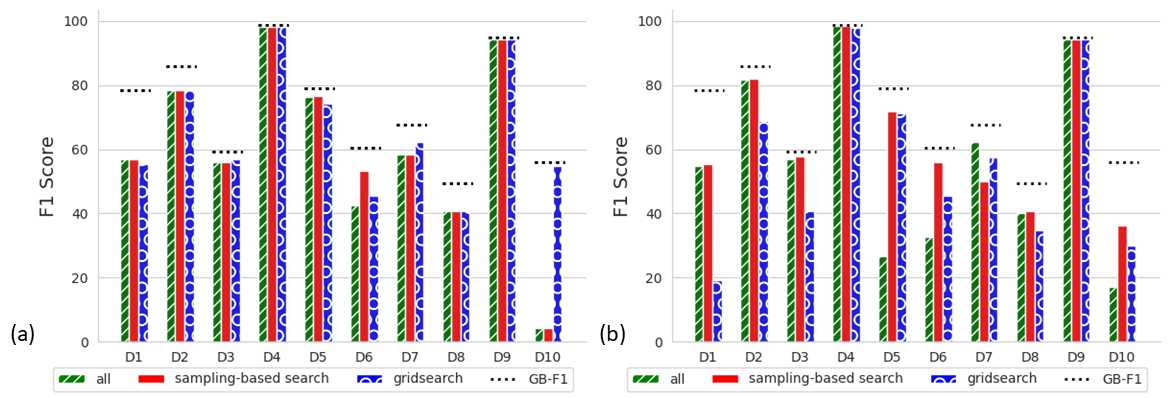
\includegraphics[width=0.9\textwidth]{Nikoletos-paper/figures/Figure7.png}
    % \vspace{-10pt}
    \caption{The F1-score of (a) the trained RF, and (b) the trained AutoML model per dataset and instance generator. GB-F1 stands for the globally best F1-score among the search algorithms in Tables \ref{tab:best-gridesearch-trials} and \ref{tab:global-bestf1s}, i.e., the performance of the best search pipeline.}
%    \vspace{-14pt}
    \label{fig:rfAutoML}
\end{figure*}
%\vspace{-3pt}
\subsection{Experimental Setup}\label{ssec:setup-p2}
For the implementation of Random Forest, we used scikit-learn v. 1.4.2\footnote{\underline{https://scikit-learn.org}}. 
For
%To implement the 
AutoML, we used auto-sklearn v. 1.4.2\footnote{\underline{https://automl.github.io/auto-sklearn}} with the following parameters: (i) The time limit in seconds for the search of appropriate models (parameter: time\_left\_for\_this\_task) was set to 12 hours. (ii) The time for a single call in the ML model (parameter: per\_run\_time\_limit) was set to 4 hours. (iii) The memory limit in MB for the machine learning algorithm (parameter: memory\_limit) equal to  24.5 GB.
%6144$\cdot$4 MB. 
(iv) The number of jobs to run in parallel (parameter: n\_jobs) was set to 1.
%No validation set used on this task, as auto-sklearn creates one internally.
All experiments were executed on a server running Ubuntu 22.04, equipped with Intel Xeon E5-4603 v2@2.2GHz and 16GB~RAM.

%\vspace{-3pt}

\subsection{Evaluation Results}
\label{sec:tackleProblem2}
%\vspace{-3pt}
To fine-tune the workflow in Figure~\ref{fig:eeter_pipeline} without any indication of matches, we apply the following procedure, resembling the leave-one-out cross-validation approach: for each dataset $D_x$ in Table~\ref{tab:dataset-specs}, we use as training set all instances generated by grid and/or sampling-based search for all other nine datasets (i.e., all datasets among $D_1$ and $D_{10}$, except $D_x$). Using these labelled instances, we train a regression model using one of the approaches in Section \ref{sec:learningProcess}. Then, we apply the learned regression model to all instances generated by the same approach for $D_x$, estimating the respective F1-score. The instance corresponding the maximum predicted F1 provides the configuration features for the ETEER pipeline that will be eventually applied to $D_x$ in order to compute the actual F1-score.

It is important to clarify the following points: 
(i) In order to find the optimal parameters, we train a model that \emph{predicts} F1-scores per configuration and picks the best one. 
(ii) After picking the best configuration, we evaluate it by computing the \emph{actual} F1 score.
(iii) Thus, we are not actually interested in the accuracy of our F1-score predictions; we are only interested in the actual F1-scores computed by using our suggested configurations.

%Note that we are not interested in measuring the accuracy of the learned model in predicting the actual F1-score per configuration; our goal is to ensure that the optimal parameter configuration is assigned the maximum predicted F1.

In this context, we address the following research questions:
\begin{enumerate}[leftmargin=*, label=RQ\arabic*), start=1]
    \item Do the three instance generation approaches in Section \ref{sec:instanceGeneration} affect the performance of the learned models?
    \item Which of the two learning processes in Section \ref{sec:learningProcess} exhibits the highest effectiveness and time efficiency?
    \item Do all features in Section \ref{sec:datasetProfiling} contribute to the effectiveness of the solutions to Problem 2?
    \item Do  our solutions to Problem 2  outperform the baseline methods w.r.t. effectiveness and time efficiency?
    \item Do our solutions to Problem 2 generalize to an unseen dataset of completely different characteristics and scale? 
    \item {How do our approaches perform in comparison to established tools for end-to-end ER that leverage syntactic similarities?}
\end{enumerate}
We elaborate on these research questions in the following.

%To address RQ4, we introduce an extra dataset (in addition to the 10 ones in Section~\ref{sec:experiments-p1}): D11, a large heterogeneous dataset which matches two different versions of DBpedia that chronologically differ by 3 years \cite{DBLP:journals/is/PapadakisMGSTGB20}.
%As baselines, we use three approaches:

%\begin{enumerate}[leftmargin=*]
%    \item The default pipeline in Table \ref{tab:best-gridesearch-trials}.
%    \item The best search pipeline, i.e., the one with the best performance for a specific dataset among the grid and sampling-based search algorithms in Tables \ref{tab:best-gridesearch-trials} and \ref{tab:global-bestf1s}, respectively. It represents the best possible performance for the ETEER pipeline of Figure~\ref{fig:eeter_pipeline}.
%    \item ZeroER \cite{DBLP:conf/sigmod/WuCSCT20}, an established ETEER approach that involves both Filtering and Verification, while requiring no labelled instances for the dataset at hand. Its performance is reported in Table \ref{tab:zeroer-results}. Note that it did not terminate in three datasets within 2 days.
%\end{enumerate}

%\begin{figure*}[t]
%    \centering
%    \begin{minipage}{0.44\linewidth}
%        \centering
%        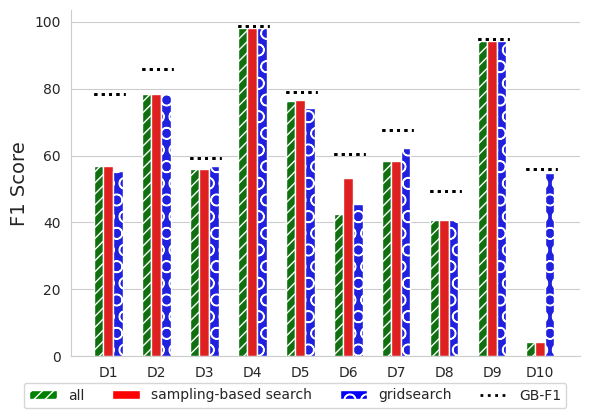
\includegraphics[width=\linewidth]{figures/predictions/sklearn_and_nn_f1.png}
        %\caption{The F1-score of the trained LR model per dataset and instance generator.}
        %\label{fig:lr-nn-f1s}
%    \end{minipage}
%    \hfill
%    \begin{minipage}{0.44\linewidth}
%        \centering
%        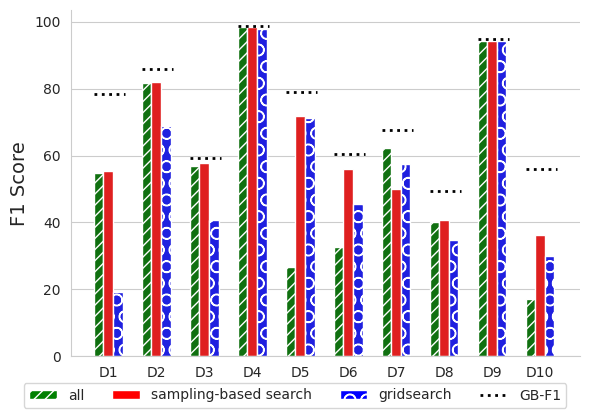
\includegraphics[width=\linewidth]{figures/predictions/autosklearn_f1.png}
        %\caption{The F1-score of the trained AutoML model per dataset and instance generator.}
%        \label{fig:autosklearnf1s}
%    \end{minipage}
%    \vspace{-10pt}
%     \caption{{\color{red}The F1-score of (a) the trained LR, and (b) the trained AutoML model per dataset and instance generator. GB-F1 stands for the globally best F1-score among the search algorithms in Tables \ref{tab:best-gridesearch-trials} and \ref{tab:global-bestf1s}, i.e., the performance of the best search pipeline.}}
%     \vspace{-10pt}
%\end{figure*}

\textbf{RQ1.} Figure \ref{fig:rfAutoML}(a) reports the F1-score of RF per dataset and instance generation approach. We observe that {the differences between the three instance generators are statistically insignificant ($p\gg0.05$ for all three pairs of generators)}. Indeed, the difference between the maximum and the minimum F1 among the three instance generators is far below 1.5\% in six of the datasets, raising to just 2.6\% and 3.6\% in $D_5$ and $D_7$, respectively. This means that there are only two datasets with significant differences between the three approaches: $D_6$, where sampling-based search takes a clear lead, and $D_{10}$, where grid search is the only approach with high performance. The extremely low performance of sampling-based search and \textit{all} on $D_{10}$ leads to \textit{grid search constituting the overall best approach for RF}, as it exhibits the highest mean F1 and the lowest variance.
%, while its distance from the globally best F1 is 10\%, on average. 
%The only exceptions appear in $D_6$ and $D_5$, where the sampling-based instances perform slightly worse and slightly better, respectively. This means that LR is able to leverage the information encapsulated in the dataset features proposed in Section \ref{sec:datasetProfiling}, regardless of the instance generator.

Much lower robustness with respect to instance generation is observed for AutoML, as shown in Figure \ref{fig:rfAutoML}(b). There is negligible deviation between the three approaches only in the two bibilographic datasets ($D_4$ and $D_9$), where the difference between the maximum and the minimum F1 is lower than 1\%. In $D_8$, this difference raises to 6\%, while in the remaining six datasets, it ranges from 12\% to 45\%. Interestingly, there is a clear winner among the three approaches: \textit{sampling-based search achieves the highest F1 in most of the datasets, while scoring the highest mean F1 and the lowest variance.} 
%On average, it also underperforms the globally best F1 by 11\%, while the other two approaches by more than 18\%.
%but $D_7$, where they rank third. In contrast, grid search instances excel in four datasets, but significantly outperform the sampling-based ones only in $D_7$.
{Indeed, the differences between sampling-based search and the other two generators are statistically significant ($p<0.05$), unlike the difference between all and grid search.}
This means that for AutoML, the 18,000 sampler instances (9 datasets $\times$ 4 search algorithms $\times$ 100 trials $\times$ 5 seeds) convey more useful information and less noise than the 359,100 grid search instances (9 datasets $\times$ 39,900 trials). 
%The combination of the two generators (``all'') typically follows the top performer or even outperforms both generators (in $D_7$).

%\begin{table*}[t]
%{\small
\begin{center}  
\caption{Performance of AutoML on Problem 2. GB stands for Gradient Boosting \cite{Friedman2001GreedyFA_GB}, KNN for K-Nearest Neighbor \cite{Fix1989DiscriminatoryA_KNN} RF for Random Forest \cite{Breiman2001RandomF_RF} and ET for Extra Trees \cite{Geurts2006ExtremelyRT_ET}. In all cases, the search/training time is 12 hours and is omitted for brevity.} 
\vspace{-10pt}
\label{tab:autosklearn-results}
%\begin{tabular}{|c|c|l|c|c|c|p{2cm}|p{1.0cm}|p{1.0cm}|c|c|c|c|}
\begin{tabular}{|c|c|l|c|c|c|c|c|c|c|}
\hline
\multirow{2}{*}{Dat.} & Inst. & \multicolumn{1}{c|}{Learned} & \multirow{2}{*}{F1} & 
%GB-F1 & F1-Ratio & 
%Optimization \& Training time (h) & 
Prediction & ETEER & \multirow{2}{*}{LM} & \multirow{2}{*}{k} & Clust & Thres \\
& gen. & \multicolumn{1}{c|}{ensemble} & & 
%GB-F1 & F1-Ratio & 
%Optimization \& Training time (h) & 
time (s) & time (s) &  &  & ering & hold \\
\hline
\hline
D1 & sampl. & 0.38ET + 0.36RF + 0.14GB + 0.1KNN + 0.02GB & 55.35 
%& 78.43 & 0.71 & 12 
& 240 & 5.84 & st5 & 1 & UMC & 0.265900 \\
D2 & sampl. & 0.82ET + 0.12GB + 0.04RF + 0.02KNN & 81.94 
%85.85 & 0.95 & 12 
& 179 & 0.18 & st5 & 1 & KC & 0.172200 \\
D3 & sampl. & 0.54ET + 0.16ET + 0.14RF + 0.12GB + 0.04KNN & 57.79 & %59.19 & 0.98 & 12 & 
218 & 2.98 & st5 & 32 & UMC & 0.05 \\
D4 & all & 0.96RF + 0.04GB & 98.45 & 
%98.60 & 1.00 & 12 & 
28 & 0.38 & st5 & 1 & CCC & 0.874200 \\
D5 & sampl. & 0.78ET + 0.1GB + 0.06RF + 0.06KNN & 71.97 & 
%78.92 & 0.91 & 12 & 
249 & 2.77 & smpnet & 1 & KC & 0.665900 \\
D6 & sampl. & 0.4ET + 0.18RF + 0.18GB + 0.12GB + 0.12KNN & 55.98 & %60.42 & 0.93 & 12 &
253 & 1.23 & sminilm & 1 & KC & 0.630700 \\
D7 & all & 0.9RF + 0.06GB + 0.04GB & 62.17 & 
%67.76 & 0.92 & 12 & 
68 & 2.05 & st5 & 1 & UMC & 0.75 \\
D8 & sampl. & 0.52ET + 0.2RF + 0.12KNN + 0.1GB + 0.06GB & 40.77 & %49.53 & 0.82 & 12 & 
230 & 20.66 & st5 & 91 & KC & 0.050100 \\
D9 & all & 0.94RF + 0.06GB & 94.39 & 
%94.92 & 0.99 & 12 & 
40 & 35.18 & st5 & 92 & KC & 0.70 \\
D10 & sampl. & 0.78ET + 0.12GB + 0.1ET & 36.31 
%& 56.12 & 0.65 & 12 
& 68 & 13.65 & smpnet & 1 & KC & 0.05 \\
\hline
\end{tabular}
\end{center}  
%}
\vspace{-10pt}
\end{table*}

%Test set & Trials training set & Regressor ensembled & F1 & GB-F1 & F1-Ratio & Optimization \& Training time (h) & Prediction time (s) & ETEER Runtime (s) & LM & k & Clustering & Threshold \\
%\midrule
%D1 & sampl. & 0.38ET + 0.36RF + 0.14GB + 0.1KNN + 0.02GB & 55.35 & 78.43 & 0.71 & 12 & 240 & 5.84 & st5 & 1 & UMC & 0.265900 \\
%D2 & sampl. & 0.82ET + 0.12GB + 0.04RF + 0.02KNN & 81.94 & 85.85 & 0.95 & 12 & 179 & 0.18 & st5 & 1 & KC & 0.172200 \\
%D3 & sampl. & 0.54ET + 0.16ET + 0.14RF + 0.12GB + 0.04KNN & 57.79 & 59.19 & 0.98 & 12 & 218 & 2.98 & st5 & 32 & UMC & 0.05 \\
%D4 & all & 0.96RF + 0.04GB & 98.45 & 98.60 & 1.00 & 12 & 28 & 0.38 & st5 & 1 & CCC & 0.874200 \\
%D5 & sampl. & 0.78ET + 0.1GB + 0.06RF + 0.06KNN & 71.97 & 78.92 & 0.91 & 12 & 249 & 2.77 & smpnet & 1 & KC & 0.665900 \\
%D6 & sampl. & 0.4ET + 0.18RF + 0.18GB + 0.12GB + 0.12KNN & 55.98 & 60.42 & 0.93 & 12 & 253 & 1.23 & sminilm & 1 & KC & 0.630700 \\
%D7 & all & 0.9RF + 0.06GB + 0.04GB & 62.17 & 67.76 & 0.92 & 12 & 68 & 2.05 & st5 & 1 & UMC & 0.75 \\
%D8 & sampl. & 0.52ET + 0.2RF + 0.12KNN + 0.1GB + 0.06GB & 40.77 & 49.53 & 0.82 & 12 & 230 & 20.66 & st5 & 91 & KC & 0.050100 \\
%D9 & all & 0.94RF + 0.06GB & 94.39 & 94.92 & 0.99 & 12 & 40 & 35.18 & st5 & 92 & KC & 0.70 \\
%D10 & sampl. & 0.78ET + 0.12GB + 0.1ET & 36.31 & 56.12 & 0.65 & 12 & 68 & 13.65 & smpnet & 1 & KC & 0.05 \\

\begin{table*}[t]
%{\small
\begin{center}  
\footnotesize  
\setlength{\tabcolsep}{2pt}
\caption{Performance of AutoML on Problem 2 when combined with sampling-based instances. GB stands for Gradient Boosting \cite{Friedman2001GreedyFA_GB}, KNN for K-Nearest Neighbor \cite{Fix1989DiscriminatoryA_KNN} RF for Random Forest \cite{Breiman2001RandomF_RF} and ET for Extra Trees \cite{Geurts2006ExtremelyRT_ET}. In all cases, the search/training time is 12 hours and is omitted for brevity.} 
% \vspace{-10pt}
{\small
\label{tab:autosklearn-results}
%\begin{tabular}{|c|c|l|c|c|c|p{2cm}|p{1.0cm}|p{1.0cm}|c|c|c|c|}
\begin{tabular}{|c|l|c|c|c|c|c|c|c|}
\hline
Dataset &  \multicolumn{1}{c|}{Learned ensemble} & F1 & 
%GB-F1 & F1-Ratio & 
%Optimization \& Training time (h) & 
Prediction time (s)& ETEER time (s)& LM & k & Clustering & Threshold \\
% & \multicolumn{1}{c|}{ensemble} & & 
%GB-F1 & F1-Ratio & 
%Optimization \& Training time (h) & 
%time (s) & time (s) &  &  & ering & hold \\
\hline
\hline
D1 & 0.38ET + 0.36RF + 0.14GB + 0.1KNN + 0.02GB & 55.35 & 240 & 5.84 & st5 & 1 & UMC & 0.2659 \\
D2 & 0.82ET + 0.12GB + 0.04RF + 0.02KNN & 81.94 & 179 & 0.18 & st5 & 1 & KC & 0.1722 \\
D3 & 0.54ET + 0.16ET + 0.14RF + 0.12GB + 0.04KNN & 57.79 & 218 & 2.98 & st5 & 32 & UMC & 0.05 \\
D4 & 0.5ET + 0.38RF + 0.08GB + 0.04KNN & 98.38 & 215 & 0.83 & st5 & 1 & KC & 0.05 \\
D5 & 0.78ET + 0.1GB + 0.06RF + 0.06KNN & 71.97 & 249 & 2.77 & smpnet & 1 & KC & 0.6659 \\
D6 & 0.4ET + 0.18RF + 0.18GB + 0.12GB + 0.12KNN & 55.98 & 253 & 1.23 & sminilm & 1 & KC & 0.6307 \\
D7 & 0.5ET + 0.24RF + 0.2GB + 0.04KNN + 0.02GB & 50.14 & 227 & 2.28 & smpnet & 1 & UMC & 0.228 \\
D8 & 0.52ET + 0.2RF + 0.12KNN + 0.1GB + 0.06GB & 40.77 & 230 & 20.66 & st5 & 91 & KC & 0.0501 \\
D9 & 0.52ET + 0.28RF + 0.14GB + 0.06KNN & 94.37 & 222 & 61.16 & st5 & 100 & KC & 0.4767 \\
D10 & 0.78ET + 0.12GB + 0.1ET & 36.31 & 68 & 13.65 & smpnet & 1 & KC & 0.05 \\
\hline
\end{tabular}
}
\end{center}  
\end{table*}
%Test set & Trials training set & Regressor ensembled & F1 & GB-F1 & F1-Ratio & Optimization \& Training time (h) & Prediction time (s) & ETEER Runtime (s) & LM & k & Clustering & Threshold \\
%\midrule
%D1 & sampl. & 0.38ET + 0.36RF + 0.14GB + 0.1KNN + 0.02GB & 55.35 & 78.43 & 0.71 & 12 & 240 & 5.84 & st5 & 1 & UMC & 0.265900 \\
%D2 & sampl. & 0.82ET + 0.12GB + 0.04RF + 0.02KNN & 81.94 & 85.85 & 0.95 & 12 & 179 & 0.18 & st5 & 1 & KC & 0.172200 \\
%D3 & sampl. & 0.54ET + 0.16ET + 0.14RF + 0.12GB + 0.04KNN & 57.79 & 59.19 & 0.98 & 12 & 218 & 2.98 & st5 & 32 & UMC & 0.05 \\
%D4 & all & 0.96RF + 0.04GB & 98.45 & 98.60 & 1.00 & 12 & 28 & 0.38 & st5 & 1 & CCC & 0.874200 \\
%D5 & sampl. & 0.78ET + 0.1GB + 0.06RF + 0.06KNN & 71.97 & 78.92 & 0.91 & 12 & 249 & 2.77 & smpnet & 1 & KC & 0.665900 \\
%D6 & sampl. & 0.4ET + 0.18RF + 0.18GB + 0.12GB + 0.12KNN & 55.98 & 60.42 & 0.93 & 12 & 253 & 1.23 & sminilm & 1 & KC & 0.630700 \\
%D7 & all & 0.9RF + 0.06GB + 0.04GB & 62.17 & 67.76 & 0.92 & 12 & 68 & 2.05 & st5 & 1 & UMC & 0.75 \\
%D8 & sampl. & 0.52ET + 0.2RF + 0.12KNN + 0.1GB + 0.06GB & 40.77 & 49.53 & 0.82 & 12 & 230 & 20.66 & st5 & 91 & KC & 0.050100 \\
%D9 & all & 0.94RF + 0.06GB & 94.39 & 94.92 & 0.99 & 12 & 40 & 35.18 & st5 & 92 & KC & 0.70 \\
%D10 & sampl. & 0.78ET + 0.12GB + 0.1ET & 36.31 & 56.12 & 0.65 & 12 & 68 & 13.65 & smpnet & 1 & KC & 0.05 \\

%\begin{table}[t]
{\small
\begin{center}  
\setlength{\tabcolsep}{2pt}
\caption{Performance of Random Forest on Problem 2.} 
\vspace{-10pt}
\label{tab:lr-with-data-features}
\begin{tabular}{|c|c|c|c|c|c|c|c|c|c|}
\hline
\multirow{2}{*}{Dat.} & Insta. & \multirow{2}{*}{F1} & Train.  & Predic.  & ETEER  & \multirow{2}{*}{LM} & \multirow{2}{*}{k} & Clust & Thre \\
 & gen. & & time (s) & time (s) &  time (s) &  &  & ering & shold \\
\hline
\hline
D1 & all & 56.77 & 0.72 & 0.02 & 2.88 & st5 & 1 & UMC & 0.73 \\
D2 & grid. & 78.46 & 0.91 & 0.01 & 5.10 & st5 & 16 & KC & 0.10 \\
D3 & grid. & 56.86 & 0.96 & 0.01 & 0.55 & st5 & 2 & KC & 0.60 \\
D4 & grid. & 98.24 & 1.00 & 0.01 & 1.70 & st5 & 2 & KC & 0.20 \\
D5 & opt. & 76.75 & 0.97 & $\ll$0.01 & 1.91 & sminilm & 1 & UMC & 0.65 \\
D6 & opt. & 53.31 & 0.88 & 0.01 & 1.34 & sminilm & 1 & KC & 0.65 \\
D7 & grid. & 62.12 & 0.92 & 0.01 & 1.58 & sminilm & 1 & KC & 0.60 \\
D8 & all & 40.78 & 0.82 & 0.01 & 28.79 & st5 & 100 & KC & 0.22 \\
D9 & all & 94.37 & 0.99 & 0.01 & 60.20 & st5 & 100 & KC & 0.38 \\
D10 & grid. & 54.91 & 0.98 & 0.01 & 37.55 & st5 & 27 & KC & 0.50 \\
\hline
\end{tabular}
\end{center}  
}
\vspace{-10pt}
\end{table}
%\toprule
% D1 & all & RFR & 56.77 & 78.43 & 0.72 & 130.55 & 1.60 & 2.88 & st5 & 1 & UMC & 0.733563 \\
% D2 & gridsearch & RFR & 78.46 & 85.85 & 0.91 & 10.10 & 0.18 & 5.10 & st5 & 16 & KC & 0.10 \\
% D3 & gridsearch & RFR & 56.86 & 59.19 & 0.96 & 10.22 & 0.18 & 0.55 & st5 & 2 & KC & 0.60 \\
% D4 & gridsearch & RFR & 98.24 & 98.60 & 1.00 & 65.26 & 1.00 & 1.70 & st5 & 2 & KC & 0.20 \\
% D5 & optuna & RFR & 76.75 & 78.92 & 0.97 & 5.25 & 0.05 & 1.91 & sminilm & 1 & UMC & 0.651879 \\
% D6 & optuna & RFR & 53.31 & 60.42 & 0.88 & 20.30 & 0.19 & 1.34 & sminilm & 1 & KC & 0.647542 \\
% D7 & gridsearch & RFR & 62.12 & 67.76 & 0.92 & 38.81 & 0.47 & 1.58 & sminilm & 1 & KC & 0.60 \\
% D8 & all & RFR & 40.78 & 49.53 & 0.82 & 27.48 & 0.29 & 28.79 & st5 & 100 & KC & 0.219945 \\
% D9 & all & RFR & 94.37 & 94.92 & 0.99 & 67.96 & 0.80 & 60.20 & st5 & 100 & KC & 0.375625 \\
% D10 & gridsearch & RFR & 54.91 & 56.12 & 0.98 & 48.67 & 0.67 & 37.55 & st5 & 27 & KC & 0.50 \\
%Test set & Trials training set & Regressor & F1 & GB-F1 & F1-Ratio & Training time (s) & Prediction time (s) & ETEER runtime (s) & LM & k & Clustering & Threshold \\
%\midrule
%D1 & all & LR & 55.35 & 78.43 & 0.71 & 0.33 & 0.01 & 0.24 & st5 & 1 & KC & 0.05 \\
%D2 & all & LR & 81.94 & 85.85 & 0.95 & 0.24 & $\ll$0.01 & 0.20 & st5 & 1 & KC & 0.05 \\
%D3 & all & LR & 55.98 & 59.19 & 0.95 & 0.33 & $\ll$0.01 & 0.48 & st5 & 1 & KC & 0.05 \\
%D4 & all & LR & 98.38 & 98.60 & 1.00 & 0.21 & $\ll$0.01 & 0.83 & st5 & 1 & KC & 0.05 \\
%D5 & all & LR & 69.39 & 78.92 & 0.88 & 0.21 & $\ll$0.01 & 0.79 & st5 & 1 & KC & 0.05 \\
%D6 & optuna & LR & 46.65 & 60.42 & 0.77 & 0.06 & $\ll$0.01 & 10.24 & st5 & 100 & KC & 0.05 \\
%D7 & all & LR & 48.48 & 67.76 & 0.72 & 0.21 & $\ll$0.01 & 1.62 & st5 & 1 & KC & 0.05 \\
%D8 & all & LR & 38.09 & 49.53 & 0.77 & 0.21 & $\ll$0.01 & 1.63 & st5 & 1 & KC & 0.05 \\
%D9 & all & LR & 92.85 & 94.92 & 0.98 & 0.21 & $\ll$0.01 & 4.23 & st5 & 1 & KC & 0.05 \\
%D10 & gridsearch & LR & 55.40 & 56.12 & 0.99 & 0.22 & 0.01 & 12.54 & st5 & 1 & KC & 0.05 \\
%\bottomrule

\begin{table}[t]
\begin{center}  
\footnotesize 
\setlength{\tabcolsep}{4pt}
\caption{Performance of Random Forest on Problem 2 when combined with grid search instances.} 
% \vspace{-10pt}
\label{tab:lr-with-data-features}
\begin{tabular}{|c|c|c|c|c|c|c|c|c|}
\hline
\multirow{2}{*}{Dat.}  & \multirow{2}{*}{F1} & Train.  & Predic.  & ETEER  & \multirow{2}{*}{LM} & \multirow{2}{*}{k} & Clust & Thre \\
 & & time (s) & time (s) &  time (s) &  &  & ering & shold \\
\hline
\hline
D1 & 55.35 & 73.10 & 1.21 & 4.11 & st5 & 1 & KC & 0.20 \\
D2 & 78.46 & 10.10 & 0.18 & 5.10 & st5 & 16 & KC & 0.10 \\
D3 & 56.86 & 10.22 & 0.18 & 0.55 & st5 & 2 & KC & 0.60 \\
D4 & 98.24 & 65.26 & 1.00 & 1.70 & st5 & 2 & KC & 0.20 \\
D5 & 74.16 & 53.34 & 0.94 & 2.05 & sminilm & 1 & KC & 0.70 \\
D6 & 45.44 & 42.50 & 0.51 & 1.20 & sminilm & 1 & KC & 0.70 \\
D7 & 62.12 & 38.81 & 0.47 & 1.58 & sminilm & 1 & KC & 0.60 \\
D8 & 40.78 & 24.27 & 0.28 & 33.10 & st5 & 99 & KC & 0.25 \\
D9 & 94.35 & 42.14 & 0.54 & 60.76 & st5 & 74 & KC & 0.35 \\
D10 & 54.91 & 48.67 & 0.67 & 37.55 & st5 & 27 & KC & 0.50 \\
\hline
\end{tabular}
\end{center}  
\end{table}
%\toprule
% D1 & all & RFR & 56.77 & 78.43 & 0.72 & 130.55 & 1.60 & 2.88 & st5 & 1 & UMC & 0.733563 \\
% D2 & gridsearch & RFR & 78.46 & 85.85 & 0.91 & 10.10 & 0.18 & 5.10 & st5 & 16 & KC & 0.10 \\
% D3 & gridsearch & RFR & 56.86 & 59.19 & 0.96 & 10.22 & 0.18 & 0.55 & st5 & 2 & KC & 0.60 \\
% D4 & gridsearch & RFR & 98.24 & 98.60 & 1.00 & 65.26 & 1.00 & 1.70 & st5 & 2 & KC & 0.20 \\
% D5 & optuna & RFR & 76.75 & 78.92 & 0.97 & 5.25 & 0.05 & 1.91 & sminilm & 1 & UMC & 0.651879 \\
% D6 & optuna & RFR & 53.31 & 60.42 & 0.88 & 20.30 & 0.19 & 1.34 & sminilm & 1 & KC & 0.647542 \\
% D7 & gridsearch & RFR & 62.12 & 67.76 & 0.92 & 38.81 & 0.47 & 1.58 & sminilm & 1 & KC & 0.60 \\
% D8 & all & RFR & 40.78 & 49.53 & 0.82 & 27.48 & 0.29 & 28.79 & st5 & 100 & KC & 0.219945 \\
% D9 & all & RFR & 94.37 & 94.92 & 0.99 & 67.96 & 0.80 & 60.20 & st5 & 100 & KC & 0.375625 \\
% D10 & gridsearch & RFR & 54.91 & 56.12 & 0.98 & 48.67 & 0.67 & 37.55 & st5 & 27 & KC & 0.50 \\
%Test set & Trials training set & Regressor & F1 & GB-F1 & F1-Ratio & Training time (s) & Prediction time (s) & ETEER runtime (s) & LM & k & Clustering & Threshold \\
%\midrule
%D1 & all & LR & 55.35 & 78.43 & 0.71 & 0.33 & 0.01 & 0.24 & st5 & 1 & KC & 0.05 \\
%D2 & all & LR & 81.94 & 85.85 & 0.95 & 0.24 & $\ll$0.01 & 0.20 & st5 & 1 & KC & 0.05 \\
%D3 & all & LR & 55.98 & 59.19 & 0.95 & 0.33 & $\ll$0.01 & 0.48 & st5 & 1 & KC & 0.05 \\
%D4 & all & LR & 98.38 & 98.60 & 1.00 & 0.21 & $\ll$0.01 & 0.83 & st5 & 1 & KC & 0.05 \\
%D5 & all & LR & 69.39 & 78.92 & 0.88 & 0.21 & $\ll$0.01 & 0.79 & st5 & 1 & KC & 0.05 \\
%D6 & optuna & LR & 46.65 & 60.42 & 0.77 & 0.06 & $\ll$0.01 & 10.24 & st5 & 100 & KC & 0.05 \\
%D7 & all & LR & 48.48 & 67.76 & 0.72 & 0.21 & $\ll$0.01 & 1.62 & st5 & 1 & KC & 0.05 \\
%D8 & all & LR & 38.09 & 49.53 & 0.77 & 0.21 & $\ll$0.01 & 1.63 & st5 & 1 & KC & 0.05 \\
%D9 & all & LR & 92.85 & 94.92 & 0.98 & 0.21 & $\ll$0.01 & 4.23 & st5 & 1 & KC & 0.05 \\
%D10 & gridsearch & LR & 55.40 & 56.12 & 0.99 & 0.22 & 0.01 & 12.54 & st5 & 1 & KC & 0.05 \\
%\bottomrule

\textbf{RQ2.} We now compare the two learning processes in combination with their best instance generation approach. The performance of Random Forest with grid search instances along with the selected workflow configurations 
%for the workflow in Figure \ref{fig:eeter_pipeline} 
is reported in Table \ref{tab:lr-with-data-features}. The same information for AutoML in combination with sampling-based instances is reported in Table \ref{tab:autosklearn-results}. We observe significant variations between the selected configurations of the two learners for each dataset.

Regarding their effectiveness, the two learners exhibit practically identical F1 score in half the datasets. In fact, the difference in their F1 score is far less than 1\% in $D_1$, $D_3$, $D_4$, $D_8$ and $D_9$. AutoML takes the lead in $D_2$ and $D_6$, while Random Forest outperforms it in the three remaining datasets. {Overall, their difference is statistically insignificant ($p = 0.50651$).} With respect to average F1 score, Random Forest takes a significant lead (66.1 vs 64.3), while exhibiting lower variance. It should be stressed that \textit{AutoML's performance depends heavily on the available search/training time}, with higher budgets yielding even better results. Yet, the current limit of 12 hours is already too high when compared to the ETEER runtime, which does not exceed 36 seconds in any of the datasets.

Regarding time efficiency, Random Forest is clearly the top performer. Its training time is consistently lower than two seconds, unlike the 12 hours required by AutoML. Its prediction time is also extremely fast, consistently requiring less than 20 milliseconds, whereas AutoML typically takes a few minutes. This should be attributed to the simpler models learned by Random Forest, unlike the complicated, weighted ensemble learned by AutoML. 

For these reasons, Random Forest trained on grid search instances is the preferred approach to tackle Problem 2 and answer RQ3. Based on RF, the overall approach for training the regression model on an existing dataset, generating the testing instances to yield a workflow configuration and applying it to a specific dataset takes less than three minutes in all datasets of Table \ref{tab:lr-with-data-features}. 

\begin{figure}[t]
    \centering
    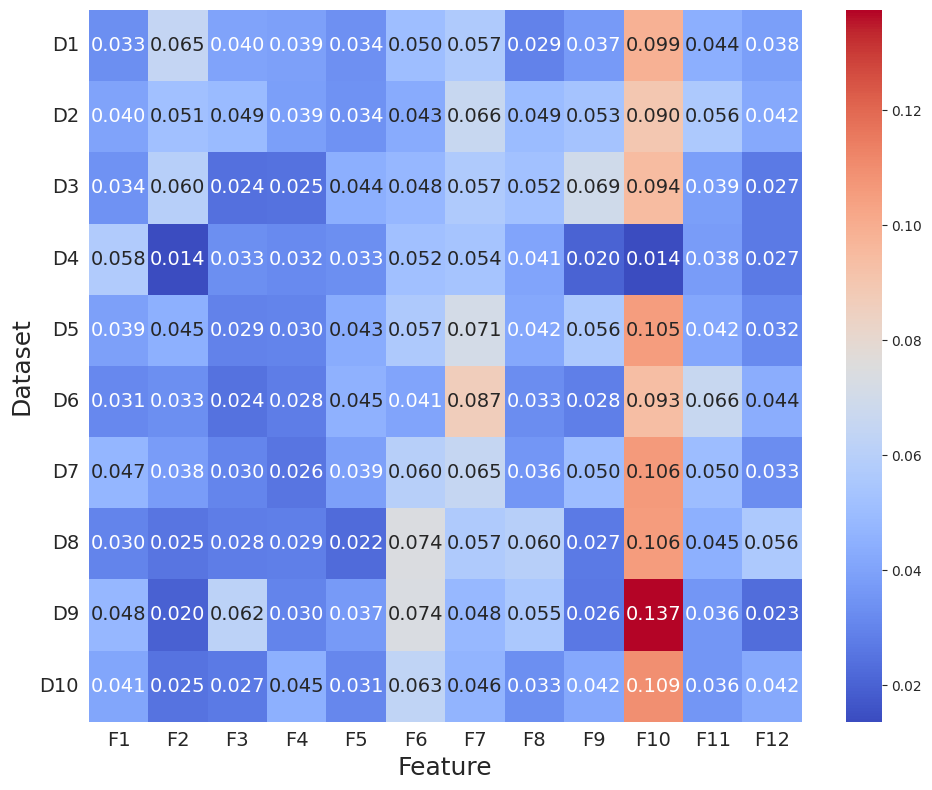
\includegraphics[width=0.85\linewidth]{Nikoletos-paper/figures/gini.png}
    % \vspace{-12pt}
    \caption{The gini importance of each feature per dataset for Random Forest with grid search instances.}
%    \vspace{-18pt}
    \label{fig:gini}
\end{figure}

\begin{table*}[t]
%\footnotesize
\centering
\setlength{\tabcolsep}{1.4pt}
\caption{Performance of ZeroER over the datasets of Table \ref{tab:dataset-specs}.}
\label{tab:zeroer-results}
\begin{tabular}{|l|c|c|c|c|c|c|c|c|c|c|}
\cline{2-11}
\multicolumn{1}{c|}{} & D1 & D2 & D3 & D4 & D5 & D6 & D7 & D8 & D9 & D10 \\
\hline
\hline
RT & 4 sec & 70 min & $\gg$48 hrs & 5.5 hrs & 34 min & $\gg$48 hrs & 67 min & $\gg$48 hrs & 24.5 hrs & 26 min \\
F1 & 0.00 & 46.46 & - & 97.00 & 92.79 & - & 88.07 & - & 64.06 & 92.62 \\
\hline
\end{tabular}
\end{table*}

\textbf{RQ3.} A major advantage of Random Forest is the interpretability of its trained decision trees, which allows for examining the specific features that are actually useful in predicting the best workflow configuration per dataset. In fact, Gini importance provides normalized estimations of the importance of each feature in $[0,1]$, with higher values indicating more important features. 

Figure \ref{fig:gini} reports this measure for all features of Section \ref{sec:datasetProfiling} across all datasets when training Random Forest with grid search instances. \textit{All features have a non-zero importance} that fluctuates between 0.137 and 0.014. On average, the most important features are F10 (0.095), F7 (0.061) and F6 (0.056), while the least important ones are F4 0.032) and F3 (0.035). Hence, \textit{despite the seemingly small variations, some features are two or even three times more important than others}. Random Forest inherently addresses these variations without requiring a specialized feature selection approach.

\begin{table*}[t]
\setlength{\tabcolsep}{3pt}
%\footnotesize
\centering
\caption{Performance over $D_{11}$ in the context of Problem 2.
%{\color{red}  ETEER Runtime (h): xana trexv ta grid,all,optuna gia na parv xronous me pre calcualated embeddings gia na mhn exei diafora me ta alla.. } 
}
% \vspace{-8pt}
\label{tab:dbpedia-results}
\begin{tabular}{|c|c|c|c|c|c|c|c|c|}
\hline
\multirow{2}{*}{LM} & \multirow{2}{*}{K} & Cluste & Thres & Training & Prediction & F1 & ETEER  & Inst. \\
 & & ring & hold& Time (h) & Time (s) & score & Runtime (h) &  gen. \\
\hline
\hline
st5 & 10 & UMC & 0.50 & - & - & 83.22 & 14.66 & - \\
\hline
\multicolumn{9}{c}{(a) Default configuration}\\
\hline
st5 & 51 & KC & 0.15 & 0.02 & 1.00 & 84.89 & 18.04 & grid \\
st5 & 1 & KC & 0.55 & 0.00 & 0.45 & 84.83 & 13.37 & sampl. \\
st5 & 100 & KC & 0.30 & 0.03 & 0.61 & 84.98 & 15.97 & all \\
\hline
\multicolumn{9}{c}{(b) Random Forest}\\
\hline
smpnet & 85 & KC & 0.55 & 12 & 17.22 & 74.26 & 16.93 & grid. \\
st5 & 1 & KC & 0.05 & 12 & 15.54 & 84.84 & 13.40 & sampl. \\
st5 & 18 & KC & 0.05 & 12 & 13.07 & 84.84 & 16.93 &  all \\
\hline
\multicolumn{9}{c}{(c) AutoML}
\end{tabular}
\vspace{-9pt}
\end{table*} 

\textbf{RQ4.} We now compare the top learned models, i.e.,  RF in combination with grid search instances and AutoML in combination with sampling-based search, with the following three baselines methods:

(i) The default pipeline in Section \ref{sec:tackleProblem1}. In most datasets, this approach underperforms both RF and AutoML to a significant extent, due to its fixed configuration. The only exception is $D_2$, where the default configuration is almost the same as the best one. AutoML performs much worse than the default configuration in $D_{10}$, too, due to the high levels of noise and the low portion of top performing configurations (see Figure \ref{fig:f1_boxplot_all}), which call for much higher search times. Overall, \textit{the adaptive workflow configurations proposed by RF and AutoML typically outperform the top-performing default one}.

(ii) The best search pipeline, i.e., GB-F1 in Figure \ref{fig:rfAutoML}, which corresponds to the best performance of the ETEER pipeline in Figure~\ref{fig:eeter_pipeline} for a specific dataset among the grid and sampling-based search algorithms in Tables \ref{tab:best-gridesearch-trials} and \ref{tab:global-bestf1s}, respectively.
%, which represents the best possible performance for the ETEER pipeline of Figure~\ref{fig:eeter_pipeline}.
%The second baseline one is the globally best F1-score among the search algorithms in Tables \ref{tab:best-gridesearch-trials} and \ref{tab:global-bestf1s} (i.e., GB-F1 in Figure \ref{fig:rfAutoML}). 
We observe that neither RF in combination with grid search instances nor AutoML in combination with sampling-based search instances outperform GB-F1 in any dataset. Yet, both RF and AutoML almost match GB-F1 in three datasets: $D_3$, $D_4$ and $D_9$. This is expected for the last two, the relatively clean bibliographic datasets, given the large portion of workflow configurations with very high performance in Figure \ref{fig:f1_boxplot_all}. For $D_{3}$, this shows the high effectiveness of both RF and AutoML. The worst performance of RF and AutoML with respect to this baseline corresponds to $D_1$ and $D_8$, where their F1-score is lower by $\sim$30\% and $\sim$20\%, respectively. These are the datasets with the lowest portion of duplicate entities, causing the selected workflow configurations to suffer from low precision. AutoML performs poorly in $D_{10}$, too, for reasons explained above.
%due to the high levels of noise and the low portion of top performing configurations (see Figure \ref{fig:f1_boxplot_all}), which call for much higher search times. 
All other datasets lie in the middle of these two extremes, with RF and AutoML underperforming GB-F1 by 10\% and 11\%, on average, respectively. 

%Random Forest, its best performance per dataset is reported in Table \ref{tab:lr-with-data-features}. It is very close to the best search pipeline in half the datasets, with LR achieving the same performance in the relatively clean bibliographic datasets, $D_4$ and $D_9$, as well as in $D_{10}$. In $D_2$ and $D_3$, its F1-score is less than 5\% lower than that of the best search pipeline. In contrast, LR underperforms almost by 30\% in $D_1$ and $D_8$, which are quite challenging, due to the very low portion of top performing configurations, as shown in Figure~\ref{fig:f1_boxplot_all}. In the remaining datasets, its F1-score is lower than the best search one by 23\% ($D_6$ and $D_8$) and 12\% ($D_5$). Overall, \textit{LR provides a performance close to the best possible one for the workflow in Figure~\ref{fig:eeter_pipeline} in most cases, while its run-time is consistently very low}, up to 21 seconds over the largest dataset, $D_{10}$. It is worth noting at this point the variety of parameter configurations proposed by LR in
%: as shown in 
%Table \ref{tab:lr-with-data-features}.
%, its overall run-time is consistently lower than the baseline methods in all datasets but $D_6$, where it uses the maximum number of candidates per query entity (100 vs 1 of the baseline methods).
%respet ETEER run-times in Table \ref{tab:best-gridesearch-trials} and most ones in Table~\ref{tab:global-bestf1s}.

(iii) ZeroER \cite{DBLP:conf/sigmod/WuCSCT20}, an established ETEER approach that involves both Filtering and Verification, while requiring no labelled instances for the dataset at hand. Its performance is reported in Table \ref{tab:zeroer-results}. Note that it did not terminate in three datasets within 2 days.
Compared to ZeroER, RF is consistently much faster: it requires far less than 3 minutes in all cases, while ZeroER requires at least 26 min in all datasets but the smallest one, where it actually finds no matches. The reason is that ZeroER cannot support missing and misplaced values, which abound in $D_1$. Apart from this dataset, RF significantly outperforms ZeroER in terms of effectiveness in three more datasets: $D_2$, $D_4$ and $D_9$. The reason is that those datasets convey long textual values, which are ideal for the pre-trained language model that lies at the core the ETEER pipeline in Figure \ref{fig:eeter_pipeline}. In contrast, $D_5$, $D_7$ and $D_{10}$ convey short textual values that usually correspond to person names. The language models struggle to find semantic similarities in these settings, unlike the string similarity measures that lie at the core of ZeroER. As a result, RF significantly underperforms ZeroER in these three datasets, but remains faster by orders of magnitude.

%Regarding AutoML, its performance is reported in Table \ref{tab:autosklearn-results}. Apart from the much higher training time (12 hours), it also raises the prediction time, due to the much more complex model that results from its learning. As a result, its performance is higher than LR in most cases, i.e., in six datasets; in $D_1$, $D_2$ and $D_4$, they yield the same F1, and only in $D_{10}$ LR performs better. Compared to the best search pipeline, the F1 score of its fine-tuned ETEER pipelines is lower by (far) less than 10\% in seven datasets. The difference is significant only in $D_1$ and $D_8$, due to the very low portion of top performing pipelines, as well as in $D_{10}$. 

Compared to ZeroER, AutoML achieves higher F1-score in the same four datasets as RF, while undeperforming in the same three datasets, for the same reason (i.e., the length of attribute values). Yet, AutoML is much worse than ZeroER in $D_5$ and $D_7$, while its run-time is significantly higher than ZeroER in all datasets, but $D_9$ (and the three datasets where ZeroER runs for more than 48 hours). 

%Overall, both RF and AutoML are capable of approximating the performance of the fine-tuned ETEER pipeline in Figure \ref{fig:eeter_pipeline} in most cases. RF emphasizes run-time, minimizing the training and prediction times, while AutoML emphasizes effectiveness. Compared to ZeroER, 
Overall, \textit{the relative effectiveness of RF and AutoML with respect to ZeroER depends on data characteristics. RF is more scalable and time efficient, while AutoML has a similar, but adjustable run-time}.
%in the case of AutoML. 

%{\color{red}It is worth noting that the overall runtime and the runtime per model, which are auto-sklearn parameters, are dependent to the resulting performance. More time provided will result probably in an even better model selected. In our experiments, we used the predefined time limits and did not further investigate the impact of longer runtimes on AutoML's ability to find the optimal model. F}

\textbf{RQ5.} In this experiment, we evaluate the generalization of the solutions to Problem 2 on $D_{11}$, a dataset with characteristics that are substantially different from all other datasets in Table \ref{tab:dataset-specs} -- unlike the limited size and schema of the other datasets, it contains millions of heterogeneous entities with user-generated content using 50,000 different attributes from two versions of DBpedia that chronologically differ by 3 years \cite{DBLP:journals/is/PapadakisMGSTGB20}.
%Wikipedia and more than \cite{DBLP:journals/is/PapadakisMGSTGB20},
Due to its size, every run of the ETEER pipeline in Figure \ref{fig:eeter_pipeline} typically takes $\sim$12 hours.
%on $D_{11}$. As a result, 
Hence, ZeroER and grid search are inapplicable,
%to this dataset, 
while the sampling-based approaches of Section~\ref{sec:problem-1} are extremely time consuming. Therefore, we use the default configuration defined in Section \ref{sec:tackleProblem1} as baseline.

Table \ref{tab:dbpedia-results} reports the performance of this baseline
%method 
along with 
%the two learning processes, i.e., 
RF and AutoML in combination with all instances generated from $D_1$-$D_{10}$ by the three approaches in Section \ref{sec:instanceGeneration}. 
%This affects only AutoML, as RF selects the same parameter configuration, regardless of the instance generator.
All tested pipelines exhibit relatively high effectiveness, with the default one matching the performance of the fine-tuned pipeline in \cite{DBLP:journals/is/PapadakisMGSTGB20}, which leverages traditional, string similarities for Filtering and Verification. This suggests that DBpedia entails many top performing configurations, like $D_4$ and $D_9$ in Figure~\ref{fig:f1_boxplot_all}. Most importantly, the configurations proposed by RF and AutoML exhibit higher F1-score by 1.6\% -- the only exception is AutoML with grid search instances, which significantly underperforms the baseline method, probably because it  requires a higher search time. This verifies the high effectiveness of the solutions to Problem 2 even in settings significantly different from the datasets generating the training instances. 

In terms of time efficiency, the prediction times of both RF and AutoML are quite low, while the run-time of the automatically configured workflows is comparable to that of the baseline.
%(default configuration). 
In fact, the sampling-based instances yield lower ETEER times by 8.9\% for both RF and AutoML. The latter, though, exhibits very high training times (12 hours), yielding a much higher overall run-time.
%Despite its higher training and prediction time and the more complex lsearned model, AutoML cannot supersede RF; in combination with sampling-based and with all instances, it exhibits the same effectiveness at the cost of higher run-times. In combination with grid search instances, the F1-score of AutoML is significantly lower.

%We can conclude, therefore, that both 
Overall, \textit{RF and AutoML 
%are able to 
can automatically configure 
%a top performing 
the ETEER pipeline even for a voluminous dataset with high levels of noise and schema heterogeneity}, with RF exhibiting very high time efficiency.
%, too.

{
\textbf{RQ6.} We now compare our approaches with two established open-source ER tools that implement end-to-end pipelines based on syntactic similarities: Magellan \cite{DBLP:journals/pvldb/KondaDCDABLPZNP16}, which involves a supervised functionality, and JedAI \cite{DBLP:journals/is/PapadakisMGSTGB20}, which operates in a learning-free way. 

For Magellan, we apply overlap blocking to the input entity collections, yielding the set of candidate pairs. These pairs are then vectorized into feature vectors, with each dimension corresponding to the score of a different similarity threshold. 80\% of these candidate pairs are automatically labelled based on the ground truth and used to train a Random Forest classifier. The trained model is then evaluated on the remaining 20\% of the candidate pairs.

For JedAI, we consider the default configuration proposed in \cite{DBLP:journals/is/PapadakisMGSTGB20} after an extensive experimental study. It consists of the following sequence of methods (note that the first two are parameter-free): (i) Token Blocking, (ii) Block Purging, (iii) Block Filtering with ratio $0.8$, (iv) CNP with the Jaccard similarity as weighting scheme, (v) Matching with character four-grams, TF-IDF weights and cosine similarity, (vi) Unique Mapping Clustering with similarity threshold~0.1.

The results are compared with the best solutions to Problems 1 and 2 in Table \ref{tab:baselines}. Starting with the best sampling-based solution to Problem 1, 
%we observe that 
its average F-Measure exceeds those of Magellan and JedAI by 5\% and 4\%, respectively. In fact, Best Sampling outperforms Magellan in half the datasets (D2-D5, D9) and exhibits almost the same performance in two others (D6, D7), with Magellan taking a major lead only in D8. Compared to JedAI, Best Sampling underperforms it only in D10, while exhibiting the same performance in D2, D3 and D4; in the remaining seven datasets, Best Sampling achieves much higher performance than JedAI.
%while dominating in seven datasets -- in the remaining datasets , they almost have .

Regarding Best AutoML and Best RF, both underperform Magellan with respect to the average F-Measure to a minor extent (by 3.7\% and 1.9\%, respectively). Looking into the individual datasets, though, we observe that there is a balance between Magellan and our approaches, as Best AutoML and Best RF are the top performers in half the datasets (D2-D5, D9). This is remarkable, when considering that Magellan requires labels for the vast majority of the candidate pairs, whereas our approaches rely exclusively on evidence from other, already labelled datasets. As a result, Best AutoML and Best RF scale easily to D11, unlike Magellan. 

\begin{table}[t]
\centering
\small 
\setlength{\tabcolsep}{2.5pt}
\caption{{The F-Measure of the best solution to Problem 1 in Table \ref{tab:global-bestf1s} (Best Sampling) and the best solutions to Problem 2 (Best AutoML from Table \ref{tab:autosklearn-results} and Best RF from Table \ref{tab:lr-with-data-features}) in comparison with 
%the main traditional end-to-end ER tools: 
Magellan \cite{DBLP:journals/pvldb/KondaDCDABLPZNP16} and JedAI \cite{DBLP:journals/is/PapadakisMGSTGB20}. In each dataset, the best performance is highlighed in bold.}}
\label{tab:baselines}
\begin{tabular}{|c|c|c|c|c|c|}
\hline
Dat. & Best Sampling & Best AutoML & Best RF & Magellan & JedAI \\
\hline
\hline
D1	& 78.43	& 55.35	& 55.35	& \textbf{84.44}	& 64.26\\
D2	& 85.85	& 81.94	& 78.46	& 43.48	& \textbf{86.73}\\
D3	& \textbf{58.97} & 57.79 & 56.86 & 45.48 & 58.65\\
D4	& \textbf{98.56} & 98.38 & 98.24 & 94.81 & 98.19\\
D5	& \textbf{78.92} & 71.97 & 74.16 & 70.51 & 67.59\\
D6	& 60.42	& 55.98	& 45.44	& \textbf{60.90} & 41.75\\
D7	& 67.76	& 50.14	& 62.12	& \textbf{67.88}	& 45.45\\
D8	& 49.53	& 40.77	& 40.78	& \textbf{63.67}	& 45.84\\
D9	& \textbf{94.92}	& 94.37	& 94.35	& 87.76	& 91.89 \\
D10	& 56.11	& 36.31	& 54.91	& 60.79	& \textbf{86.94} \\
%D11 & - & 84.84 & \textbf{84.98}  & - & 81.31 \\
\hline
\hline
Mean & 72.95 & 64.30 & 66.07 & 67.97 & 68.73 \\
\hline
\end{tabular}
\end{table}

Finally, comparing JedAI with Best AutoML and Best RF, we observe that the former achieves a higher average F-Measure only because of the extremely higher performance on D10. Excluding D10, the relative performance is reversed, with our approaches outperforming JedAI by at least 0.6\%: 66.71 for JedAI vs 67.41 for Best AutoML and 67.31 for Best RF. The advantage of our approaches becomes greater when considering D11, too, where JedAI underperforms them by 3.6\% (81.3 vs 84.9 for our approaches). Looking at the individual datasets, we observe that there is a balance between JedAI and our approaches. They all have almost the same performance on D4, with JedAI being the top performer in 5 datasets and our approaches in the remaining five ones (including D11). Apart from the high performance, Best AutoML and Best RF have a qualitative advantage, as their functionality is adaptive, depending on the characteristics of the input data, unlike JedAI, which applies the same pipeline to all datasets.

On the whole, our approaches significantly outperform Magellan and JedAI when labelled data is available, otherwise they offer similar levels of performance. In the latter case, though, they scale well to large datasets, unlike Magellan, while providing an adaptive, data-driven functionality, unlike JedAI.
}

\textbf{Conclusions.} Both RF and AutoML 
%Our methodology to addressing Problem 2 
are capable of fine-tuning the ETEER pipeline in Figure \ref{fig:eeter_pipeline} under versatile settings. Using the former (ideally with grid search instances), the training and prediction times are minimized, while the proposed configuration typically achieves higher effectiveness than the one proposed by AutoML, despite its time-consuming search phase. 
%the  performs very well in most cases. AutoML trades significantly higher effectiveness for much higher training and prediction times, but this can be adjusted according to the available time and memory.%temporal resources.

%=================================
%As outlined in Section~\ref{sec:learningProcess}, when the ground truth is not available, we employed two different approaches. The primary strategy for tackling Problem 2 was to utilize the trials conducted for Problem 1, in conjunction with a set of data features extracted from the datasets to be matched. We organized the experiments for this task by first dividing the trials from Problem 1 into three distinct categories: \textit{Optuna}, which comprises the combined trials from all four Optuna samplers; \textit{Gridsearch}, which consists of all trials from the comprehensive grid search benchmarking; and \textit{all}, which is the amalgamation of both the \textit{Optuna} and \textit{Gridsearch} trials. Using these three sets, we trained models on each set following the two learning procedures described in Section~\ref{sec:learningProcess}. Specifically, we obtained 52,500 trials from each sampler, totaling 5*52,500 = 210,000 trials for the \textit{Optuna} set. The \textit{Gridsearch} set contained 399,000 trials (39,900 trials for each of the 10 datasets). Combining these, the \textit{all} set comprised 609,000 trials.
%For all the training experiments, trials with an F1-score of zero were excluded from the training sets. Additionally, duplicate trials, where samplers proposed configurations already covered by the grid search, were also removed from the training sets. 
% \begin{figure}[h!]
%     \centering
%     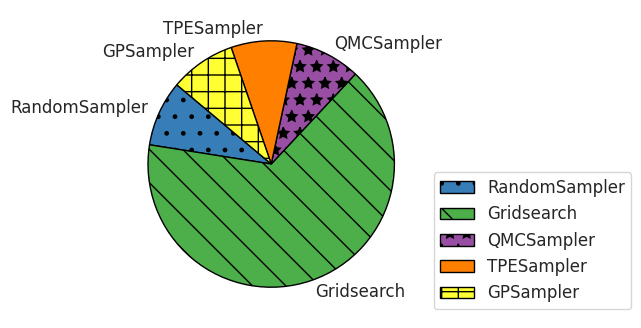
\includegraphics[width=\linewidth]{figures/predictions/sampler_distribution.png}
%     \caption{All trials training set distribution.}
%     \label{fig:sampler-distributions}
% \end{figure}



%\begin{table*}[ht!]
\centering
\caption{Default F1s for pipeline (st5, 10, UniqueMappingClustering, 0.5).}
\label{tab:global-bestf1s}
\begin{tabular}{|c|c|c|}
\toprule
Dataset & F1 & Runtime (s)\\
\midrule
D1 & 47.44 & 1.90 \\
D2 & 85.85 & 3.28 \\
D3 & 57.35 & 1.49 \\
D4 & 97.56 & 4.45 \\
D5 & 57.74 & 5.05 \\
D6 & 30.39 & 1.81 \\
D7 & 35.68 & 2.21 \\
D8 & 35.82 & 4.46 \\
D9 & 92.04 & 13.11 \\
D10 & 53.63 & 27.96 \\
\bottomrule
\end{tabular}
\end{table*}


%\subsubsection{AutoML learning procedure}

%Using auto-sklearn, we conducted experiments by withholding one dataset as the test set while training the AutoML models on all remaining datasets. The results of this approach are summarized in Table \ref{tab:autosklearn-results}, where we present the best experiments for each dataset. The column labeled \textit{Test set} indicates the dataset used as the test set, while all others served as training sets. The \textit{Trials} column lists the set of trials used for each experiment. \textit{Predicted F1} refers to the actual F1-score of the predicted configuration, measured using pyJedAI. \textit{GB-F1} represents the highest F1-score obtained by any method for each dataset, and \textit{Performance} measures how close the ETEER prediction was to the best F1-score. 
%\comments{psiliazomai, mallon swsta, ti einai to performance. mipws na dwseis ton tupo pou xreisimopoieis? vasilis: sigoura!}

%\begin{table*}[ht!]
{\footnotesize
\begin{center}  
\caption{Learning procedure 1 (AutoML) results. \textbf{WITHOUT Data Features.} GB:Gradient Boosting, RF:Random Forest, ET:Extra Trees, KNN:K-Nearest Neighbor, AD:AdaBoost, ARD:ARD Regression } 
\label{tab:autosklearn-results}
\begin{tabular}{|c|c|p{2.5cm}|c|c|c|p{2cm}|p{1.0cm}|p{1.0cm}|c|c|c|c|}
\toprule
Test set & Trials training set & Regressor ensembled & F1 & GB-F1 & F1-Ratio & Optimization \& Training time (h) & Prediction time (s) & ETEER Runtime (h) & LM & k & Clustering & Threshold \\
\midrule
D1 & all & 0.54GB + 0.36RF + 0.1GB & 57.14 & 78.43 & 0.73 & 12 & 62 & 12.02 & st5 & 1 & KMAC & 0.7790 \\
D2 & optuna & 0.92ET + 0.02ET + 0.02GB + 0.02KNN + 0.02AD & 78.63 & 85.85 & 0.92 & 12 & 61 & 12.02 & st5 & 12 & KMAC & 0.111700 \\
D3 & all & 0.62GB + 0.36RF + 0.02GB & 57.42 & 59.19 & 0.97 & 12 & 56 & 12.01 & st5 & 100 & KMAC & 0.3017 \\
D4 & all & 0.66GB + 0.32RF + 0.02GB & 98.18 & 98.60 & 1.00 & 12 & 69 & 12.02 & st5 & 21 & KMAC & 0.3019 \\
D5 & gridsearch & 0.72RF + 0.14AD + 0.12ARD + 0.02AD & 72.87 & 78.92 & 0.92 & 12 & 17 & 12.00 & st5 & 81 & KMAC & 0.70 \\
D6 & optuna & 0.86ET + 0.04ET + 0.04GB + 0.04KNN + 0.02ARD & 51.16 & 60.42 & 0.85 & 12 & 56 & 12.02 & sminilm & 1 & UMC & 0.20 \\
D7 & all & 0.58GB + 0.36RF + 0.06GB & 65.47 & 67.76 & 0.97 & 12 & 68 & 12.02 & sminilm & 1 & UMC & 0.6694 \\
D8 & optuna & 0.9ET + 0.02GB + 0.02AD + 0.02KNN + 0.02RF + 0.02RF & 47.05 & 49.53 & 0.95 & 12 & 62 & 12.02 & st5 & 1 & UMC & 0.8960 \\
D9 & optuna & 0.86ET + 0.1RF + 0.04GB & 94.39 & 94.92 & 0.99 & 12 & 25 & 12.02 & st5 & 21 & KMAC & 0.3019 \\
D10 & all & 0.6GB + 0.36RF + 0.04GB & 55.40 & 56.12 & 0.99 & 12 & 50 & 12.01 & st5 & 1 & KMAC & 0.1932 \\
\bottomrule
\end{tabular}
\end{center}  
}
\end{table*}


%Among all AutoML attempts, implementations of Gradient Boosting and Extra Trees models consistently showed the best performance. Additionally, using the \textit{all} trials set yielded the best results for 6 out of 10 datasets. However, it is also notable that the \textit{Optuna} trials sets produced the best results in 4 out of 10 datasets.

%The configurations predicted by AutoML achieved near-optimal F1-scores, particularly for datasets D2, D3, D4, D5, D7, and D9, with the minimum \textit{Performance} being 69\% "close" to the best F1-score. To further illustrate the results of this learning procedure, Figure \ref{fig:autosklearn-f1s} provides a comparative analysis of all datasets across all trial sets. There is no significant distinction between the sets of trials, as they exhibit similar performance, which is encouraging as it suggests robustness across different trial sets.
%\comments{Sto d2 kai d10 exoume kapoies diafores. eksigise giati. kapoia xaraktiristika twn datasets isws?}



%It is worth noting that the overall runtime and the runtime per model, which are auto-sklearn parameters, are dependent to the resulting performance. More time provided will result probably in an even better model selected. In our experiments, we used the predefined time limits and did not further investigate the impact of longer runtimes on AutoML's ability to find the optimal model.

%\comments{genika den sxoliazeis ka8olou kati metaksu twn datasets. kati na pros8esoume? epireazoun px ta features sto section 5.1?}

%\subsubsection{Individual regressors learning procedure}

%In a different manner, we also employed another learning procedure with quite a different methodology. We tested classic regressors provided from sklearn open-source python toolkit, while also created a naive Neural Network to test it for this task. A validation set of size 10\% from all training data trials is created, and using this we try to minimize the MSE using Optuna as a hyperparameter tool. To better understant this technique please revisit Section \ref{sec:learningProcess} and Learning Procedure 2. The exact configuarations tested can be found in Appendix and Table \ref{tab:parameter-values}. 

% \begin{table}[t]
{\footnotesize
\begin{center}  
\caption{Learning Procedure 2 results (Individual regressors).}
\label{tab:sklearn-nn-results}
\begin{tabular}{|p{0.5cm}|l|p{1.2cm}|p{1.2cm}|p{1cm}|l|}
\hline
\textbf{Test set} & \textbf{Trials} & \textbf{Regressor} & \textbf{Predicted F1} & \textbf{Best F1} & \textbf{Performance} \\
\hline
D1 & optuna & RFR & 56.77 & 78.43 & 0.72 \\
D2 & gridsearch & NN & 85.40 & 85.85 & 0.99 \\
D3 & gridsearch & XGB & 56.88 & 59.19 & 0.96 \\
D4 & all & NN & 98.51 & 98.60 & 1.00 \\
+D5 & optuna & RFR & 76.96 & 78.92 & 0.98 \\
D6 & optuna & XGB & 51.81 & 60.42 & 0.86 \\
D7 & all & RFR & 64.24 & 67.76 & 0.95 \\
D8 & all & RFR & 40.78 & 49.53 & 0.82 \\
D9 & all & RFR & 94.37 & 94.92 & 0.99 \\
D10 & all & LR & 55.80 & 56.12 & 0.99 \\
\bottomrule
\end{tabular}
\end{center}  
}
\end{table}

%\begin{table*}[ht!]
{\footnotesize
\begin{center}  
\caption{Learning procedure 2 (Linear Regression) results. \textbf{WITHOUT Data Features.}} 
\label{tab:lr-without-data-features}
\begin{tabular}{|c|c|c|c|c|c|c|c|c|c|c|c|c|}
\toprule
Test set & Trials training set & Regressor & F1 & GB-F1 & F1-Ratio & Training time (s) & Prediction time (s) & ETEER Runtime (s) & LM & k & Clustering & Threshold \\
\midrule
D1 & optuna & LR & 55.35 & 78.43 & 0.71 & 0.02 & 0.00 & 0.02 & st5 & 1 & KMAC & 0.05 \\
D2 & optuna & LR & 81.94 & 85.85 & 0.95 & 0.02 & 0.00 & 0.02 & st5 & 1 & KMAC & 0.05 \\
D3 & optuna & LR & 55.98 & 59.19 & 0.95 & 0.02 & 0.00 & 0.02 & st5 & 1 & KMAC & 0.05 \\
D4 & all & LR & 98.38 & 98.60 & 1.00 & 0.08 & 0.00 & 0.078 & st5 & 1 & KMAC & 0.05 \\
D5 & optuna & LR & 69.39 & 78.92 & 0.88 & 0.02 & 0.00 & 0.02 & st5 & 1 & KMAC & 0.05 \\
D6 & optuna & LR & 43.85 & 60.42 & 0.73 & 0.02 & 0.00 & 0.022 & st5 & 1 & KMAC & 0.05 \\
D7 & optuna & LR & 48.48 & 67.76 & 0.72 & 0.02 & 0.00 & 0.022 & st5 & 1 & KMAC & 0.05 \\
D8 & optuna & LR & 38.09 & 49.53 & 0.77 & 0.02 & 0.00 & 0.022 & st5 & 1 & KMAC & 0.05 \\
D9 & optuna & LR & 92.85 & 94.92 & 0.98 & 0.02 & 0.00 & 0.022 & st5 & 1 & KMAC & 0.05 \\
D10 & gridsearch & LR & 55.40 & 56.12 & 0.99 & 0.04 & 0.00 & 0.04 & st5 & 1 & KMAC & 0.05 \\
\bottomrule
\end{tabular}
\end{center}  
}
\end{table*} 


%Table \ref{tab:sklearn-nn-results}, shows the performance of this learning procedure. Again Random Forest is shown to be quite effective. In contrast with AutoML experiment, more trials (i.e. \textit{All} training set) yields in 6 out of 10 the best results. In a same way like the previous experiment, we provide Figure \ref{fig:sklearn-nn-f1s}, where again we notice no big differnece between sets of trials. It is now evident that no matter the trials set we will get a similar scrore, making Optunas trials set, really appealing as it has less than half the size of \textit{All} trials set.


% \subsubsection{Comparative analysis ??}

% \begin{table}[ht!]
\caption{All results (to be removed).}
\label{tab:dl-results}
\begin{tabular}{|p{0.5cm}|l|p{1.2cm}|p{1.2cm}|p{1cm}|l|}
\hline
\textbf{Test set} & \textbf{Dataset} & \textbf{Regressor} & \textbf{Predicted F1} & \textbf{Best F1} & \textbf{Perfo} \\
\hline
% \midrule
D1 & optuna & RFG & 56.77 & 78.43 & 0.72 \\
D2 & gridsearch & NN & 85.40 & 85.85 & 0.99 \\
D3 & all &  AutoGB & 57.42 & 59.19 & 0.97 \\
D4 & all & NN & 98.51 & 98.60 & 1.00 \\
D5 & optuna & RFG & 76.96 & 78.92 & 0.98 \\
D6 & optuna & XGB & 51.81 & 60.42 & 0.86 \\
D7 & all & RFG & 64.24 & 67.76 & 0.95 \\
D8 & all & RFG & 40.78 & 49.53 & 0.82 \\
D9 & optuna &  AutoET & 94.39 & 94.92 & 0.99 \\
D10 & all & LR & 55.80 & 56.12 & 0.99 \\
\bottomrule
\end{tabular}
\end{table}     


% \begin{figure}[h!]
%     \centering
%     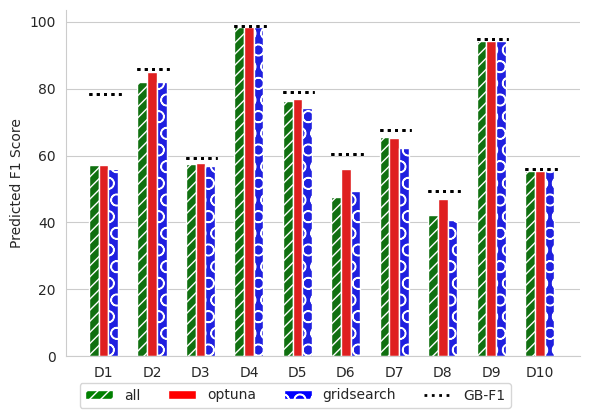
\includegraphics[width=0.99\linewidth]{figures/predictions/all_f1.png}
%     \caption{All F1-scores.}
%     \label{fig:all-f1s}
% \end{figure}


\vspace{-5pt}
\section{Related Work}\label{sec:related_work}

%In~\cite{DBLP:conf/bigdataconf/EfthymiouIKKMNPSVZ23}, we envisioned a self-configurable, end-to-end ER framework that can operate in different domains, focusing on geo-spatial interlinking, while also supporting ethical constraints, like fairness. As a follow-up to this work, we are now providing a practical implementation of many of those envisioned features, leaving out domain adaptations and ethical considerations, as they are orthogonal to the topic of this work.

%\textbf{Auto-ER Approaches.} 
\textbf{Entity Resolution.} There has been limited research on automatically configuring 
%Entity Resolution (
ER pipelines, with most relevant works
%and ER problems in general. Most existing work on auto-configuring ER 
focusing on the Entity Matching step ( i.e., on Verification), rather than end-to-end ER, as in our case. More specifically, 
%the study in introduces 
a transfer-learning framework that utilizes pre-trained Entity Matching models derived from extensive knowledge bases (KBs) is proposed in \cite{AutoER_WWW}. However, this approach is domain-specific, heavily relying on relevant and well-curated KBs, which limits its applicability in real-world scenarios where such KBs are unavailable. In contrast, our ETEER methodology is domain-agnostic and holistic, also covering Filtering, and can be applied across various data types. 
%{\color{red}Is it only about matching?}

%Another study  attempts 
Another approach to constructing a purely automatic 
%AutoML 
Entity Matching pipeline using AutoML is presented in \cite{AutoER_EDBT}, which uses auto-sklearn to predict whether a pair of entities is a match/non-match by transforming the textual description of entities through BERT-based pre-trained language models. It differs from the tasks examined in our work in that it completely disregards Filtering.
%This approach yields suboptimal results compared to ETEER; for example, the highest F1 score achieved in dataset D2 is 66.37\%, while ETEER achieves 85.39\%. 

Lastly, the 
%AutoML-EM 
framework in \cite{AutoER_ICDE}
%, which shares similarities with our approach by using 
uses AutoML models to predict the optimal Random Forest configuration. Again, it disregards Filtering, treating it as an orthogonal problem, while the proposed solution %However, this work 
is limited to a specific type of classifier for Verification. It relies on an active learning and self-training strategy, which necessitates a human-in-the-loop algorithm when ground truth pairs are scarce. In contrast, our ETEER methodology requires no human involvement.

%\textbf{ER Tools.} Several ER tools are designed to require minimal or no configuration. Some of the most hands-off approaches are described in papers like \cite{}. For example, Ditto \cite{DBLP:journals/pvldb/0001LSDT20} extends the BERT-based EMTransformer by integrating external, domain-specific knowledge, such as Part-of-Speech (POS) tagging, and employing data augmentation techniques to create synthetic training instances. However, Ditto requires configuration of several deep learning parameters, such as learning rate and epochs. Similarly, DeepMatcher \cite{DEEPMATCHER} is a comprehensive framework for deep learning-based matching algorithms, supporting various pre-trained static embeddings, including GloVe and FastText, with FastText as the default choice. While DeepMatcher involves fewer configuration parameters, users still need to specify word embeddings, and no auto-configuration component has been proposed. Finally, ZeroER \cite{DBLP:conf/sigmod/WuCSCT20} is an unsupervised-learning approach, used for ER with almost none parameters to be configured \textcolor{red}{(maybe we should compare it with P1?)},

%\textbf{Hyperparameter Optimization Frameworks.} Several toolkits have been developed for automatically configuring hyperparameters, such as SMAC \cite{AUTOCONF:Lindauer_SMAC3_A_Versatile_2022}, Hyperopt \cite{AUTOCONF:hyperopt}, Autotune \cite{AutoTune}, and Vizier \cite{oss_vizier, google_vizier}. These frameworks utilize various algorithms for parameter sampling, which selects combinations of parameters from a predefined search space. For instance, Spearmint \cite{SpearMint:NIPS2012_05311655} uses Gaussian Processes, while Hyperopt employs the tree-structured Parzen estimator (TPE). SMAC \cite{AUTOCONF:Lindauer_SMAC3_A_Versatile_2022} introduced a method based on random forests. More recent frameworks, such as Google Vizier \cite{oss_vizier, google_vizier} and Tune \cite{AutoTune}, incorporate pruning algorithms, which aim to minimize the search time: they assess the intermediate outcomes of each trial and terminate as soon as the trial is not in the top-k most promising trials ranking, thereby accelerating the configuration search process. This is akin to the early-stopping technique commonly used in various machine learning tasks.

{
\textbf{Entity Alignment.} ER is similar to Entity Alignment (EA), which focuses on detecting matching entities across two knowledge graphs (KGs) \cite{DBLP:books/sp/ZhaoZT23}. In this context, a work similar to ours is presented in \cite{DBLP:conf/dasfaa/ZengZTLLZ21}, which proposes \textsf{UEA}, an unsupervised approach that requires no labelled instances. \textsf{UEA} computes the semantic and syntactic distances of entity names, while taking special care to detect and filter out entities that appear only in one of the two input KGs. This information is then combined with structural evidence about neighboring entities from graph convolutional networks, generating preliminary aligned pairs. These pairs are progressively augmented to improve the quality of KG embeddings and enhance the alignment performance. A gradually increasing threshold is used to distinguish between the matching and non-matching pairs in each iteration.

Another similar EA approach,  CEAFF\cite{DBLP:journals/tois/ZengZTLG21}, combines complementary evidence from structural, semantic and string-level features through a novel adaptive strategy that generates a fused similarity matrix. This matrix is then used for taking collective alignment decisions that consider the neighbors of the matched entities, while taking into account the coherence and exclusiveness constraints through the framework's reward.

Unfortunately, these works cannot be adapted to ER, because they rely on the structural information of KGs involved in EA. This kind of information is rarely available in ER, which may integrate flat, relational or even unstructured data that lack any structural information.

\textbf{AutoML.} AutoML is the research field that aims to democratize the creation of ML pipelines, allowing even novice users to automatically build powerful solutions \cite{DBLP:books/sp/HKV2019}. First, it identifies the design choices and then, it generates performance-optimized models through a search strategy that optimizes hyperparameters \cite{DBLP:journals/air/BaratchiWLRHBO24}. The latest developments in this field include EDCA \cite{DBLP:conf/evoapps/SimoesC25}, a framework that improves energy and time efficiency by combining genetic algorithms with data quality techniques,  reinforcement learning for neural architecture search and hyperparameter optimization, e.g., through Sequential Policy Gradient modeling, \cite{DBLP:journals/corr/abs-2506-15051}, as well as efforts to improve AutoML approaches with guidance from LLMs \cite{DBLP:journals/tmlr/TornedeDEGMRSTT24}, e.g., for hyperparameter optimization \cite{DBLP:journals/corr/abs-2312-04528} and for Graph Neural Architecture Search \cite{DBLP:journals/corr/abs-2502-10459}. 

To the best of our knowledge, this work is the first to apply AutoML techniques to ER,  confining the search space to the configuration space of the end-to-end pipeline in Figure~\ref{fig:eeter_pipeline}, while using the ER evaluation measures for assessing its performance. For hyperparameter optimization, we use sampling algorithms in case the ground truth is available and trained ML models in case it is not. We can replace these search algorithms with any other from the literature.
}
\vspace{-5pt}
\section{Conclusion}\label{sec:conclusion}

We have defined two problems for auto-configuring end-to-end entity resolution (ETEER) pipelines: one applicable to datasets for which some known matches are available for training, and another one for a setting in which there is no ground truth of matches for the given dataset. We adapted existing techniques to solve each problem, based on a state-of-the-art ETEER pipeline.

For the first problem, we adapt established search algorithms for hyperparameter optimization to ETEER. Our thorough experimental analysis over 10 popular real-world datasets demonstrates that these algorithms match or exceed the effectiveness of grid search, while reducing the number of trials and the corresponding search time by 2 or even 3 orders of magnitude. 

For the second problem, we consider 12 generic features that can be efficiently extracted from each dataset, regardless of its format and ER setting. To learn the relations between these features, labelled instances are generated from datasets with an available ground truth and used to train a regression model using Random Forest (RF) or AutoML -- both are state-of-the-art learning algorithms that inherently perform feature selection. 
Experiments over 11 real-world datasets demonstrate the high importance of most features, with the best performance in terms of effectiveness and time efficiency corresponding to RF with grid search instances. 

In the future, we plan to generalize our approach so that it is independent of the ETEER pipeline: given a dataset, we should be able to recommend the best pipeline (not necessarily the one in Figure \ref{fig:eeter_pipeline}) along with its best hyperparameters.

\section*{Acknowledgements}
This work was partially funded by the EU project STELAR (Horizon Europe -- Grant No. 101070122).





















% %\begin{itemize}
%     %\item Add all pyjedai pipelines. Maybe in parallel, and 3 separate best configurations
%     %\item Repeat for more datasets
% %\end{itemize}

% We have defined two problems for fine-tuning ETEER pipelines: one aiming to identify the best configuration parameters in datasets with known ground truth, one in datasets without any knowledge about the true matches. Based on a specific, state-of-the-art ETEER pipeline, we adapted existing techniques to solve each problem. 

% For the first one, we adapt to ETEER existing established search algorithms for hyperparameter optimization. Our thorough experimental analysis over 10 popular datasets demonstrates that these algorithms match or exceed the effectiveness of grid search even though they reduce the number of trials and the corresponding search time by 2 or even 3 orders of magnitude. 

% For the second problem, we consider
% %propose a dataset profiling approach that extracts 
% 12 generic, efficient and effective features that are extracted from each dataset, regardless of its format and type of ER. To learn the relations between these features, labelled instances are generated from datasets with an available groundtruth and used to train a regression model using Random Forest or AutoML -- both are state-of-the-art learning algorithms that inherently perform feature selection. 
% %The model can be simple, leveraging linear regression (LR), or complex, leveraging a linear combination of individual regressors, based on AutoML. Our 
% Experiments over 11 real-world datasets demonstrate the high importance of most features, with the best performance in terms of effectiveness and time efficiency corresponding to RF with grid search instances. 
% %of our methodology as well as a clear trade-off between the two regression models: LR trades slightly lower F1 for significantly higher time efficiency (i.e., lower training and prediction times), and vice versa for AutoML.

% In the future, we plan to generalize our approach so that it is independent of the ETEER pipeline: given a dataset, we should be able to recommend the best pipeline (not necessarily the one in Figure \ref{fig:eeter_pipeline}) along with its best hyperparameters.

% %Future work: Only receive the entity collections as input and suggest not just the best configurations, but also the best pipeline. 

\bibliographystyle{IEEEtran}
\bibliography{sample}

\begin{IEEEbiography}[{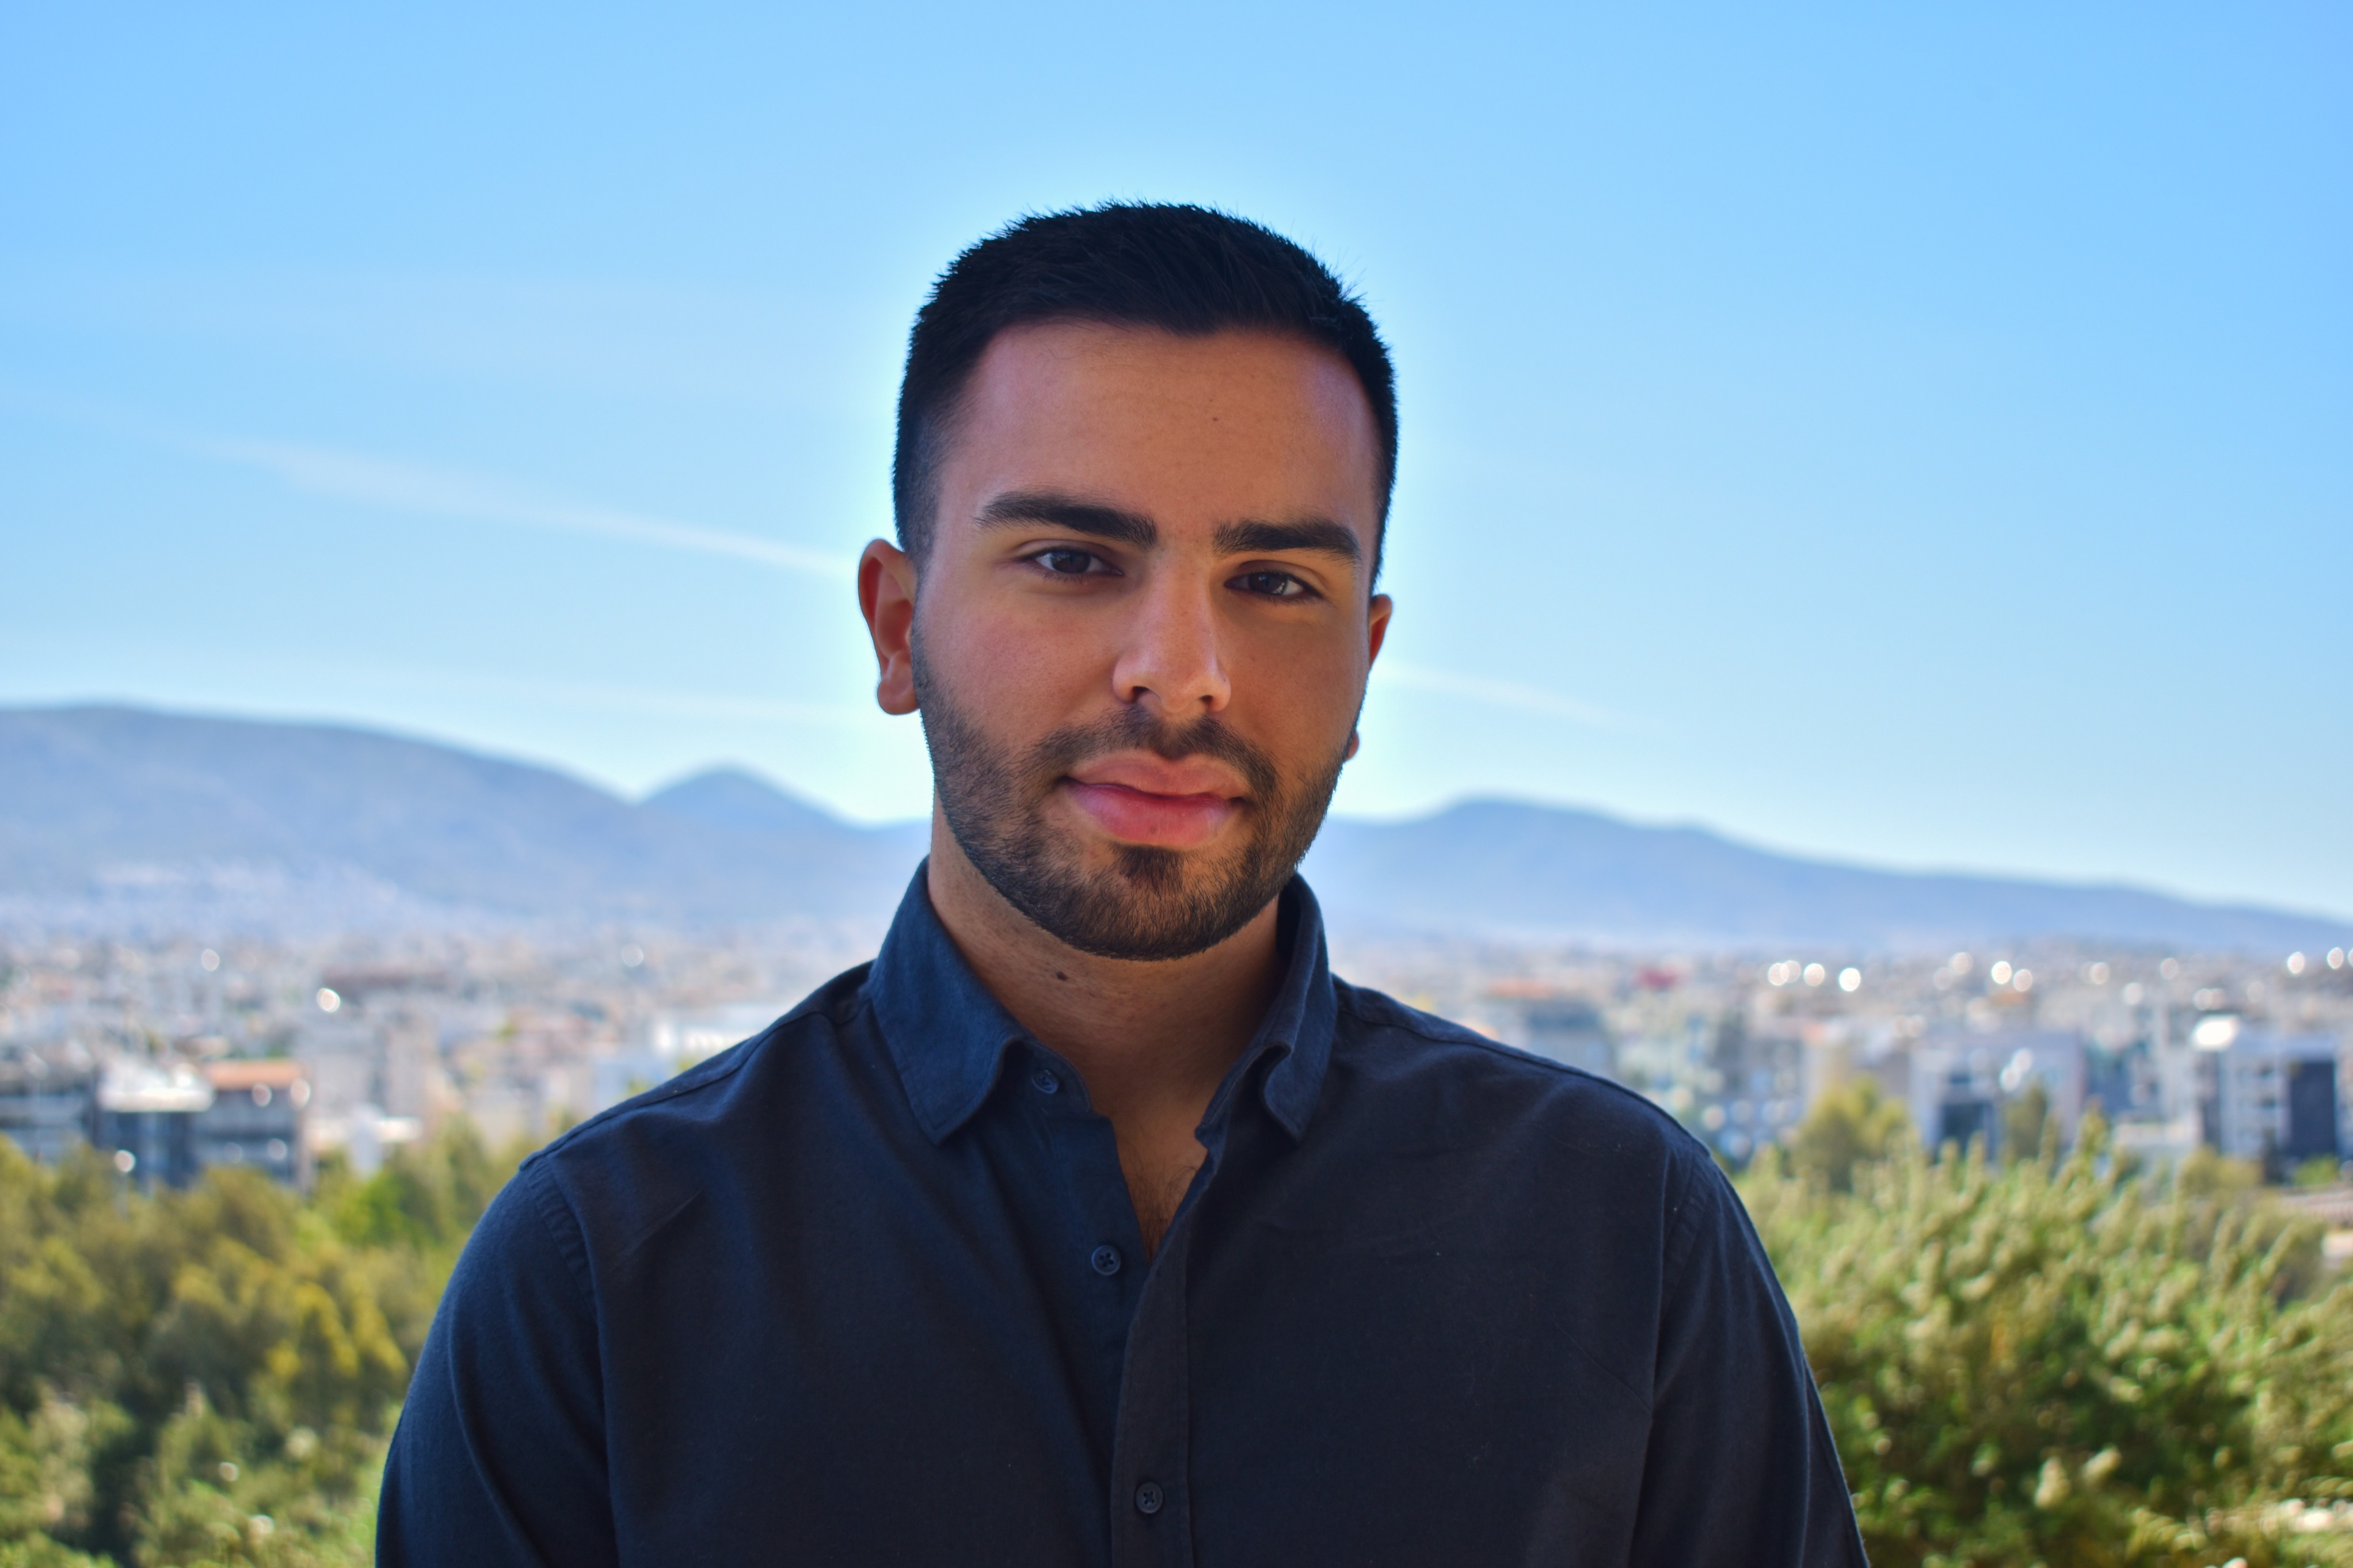
\includegraphics[width=1in,height=1.25in,clip,keepaspectratio]{Nikoletos-paper/profiles-pics/nikoletos.png}}]{Konstantinos Nikoletos} is a PhD candidate at Utrecht University and an affiliate researcher at University of Athens and the University of Trento. He holds a B.Sc. (2022) and an M.Sc. (2024) in Computer Science from the University of Athens, with a specialization in Data, Information, and Knowledge Management. Before joining Utrecht University, he has been for several years, a member of the AI Team at the University of Athens. In-between he served as a Research Fellow at the University of Trento Italy, where he remains an active member. His expertise focuses on Data Management, Entity Resolution and Data Sustainability.
\end{IEEEbiography}
\vspace{-30pt}
\begin{IEEEbiography}[{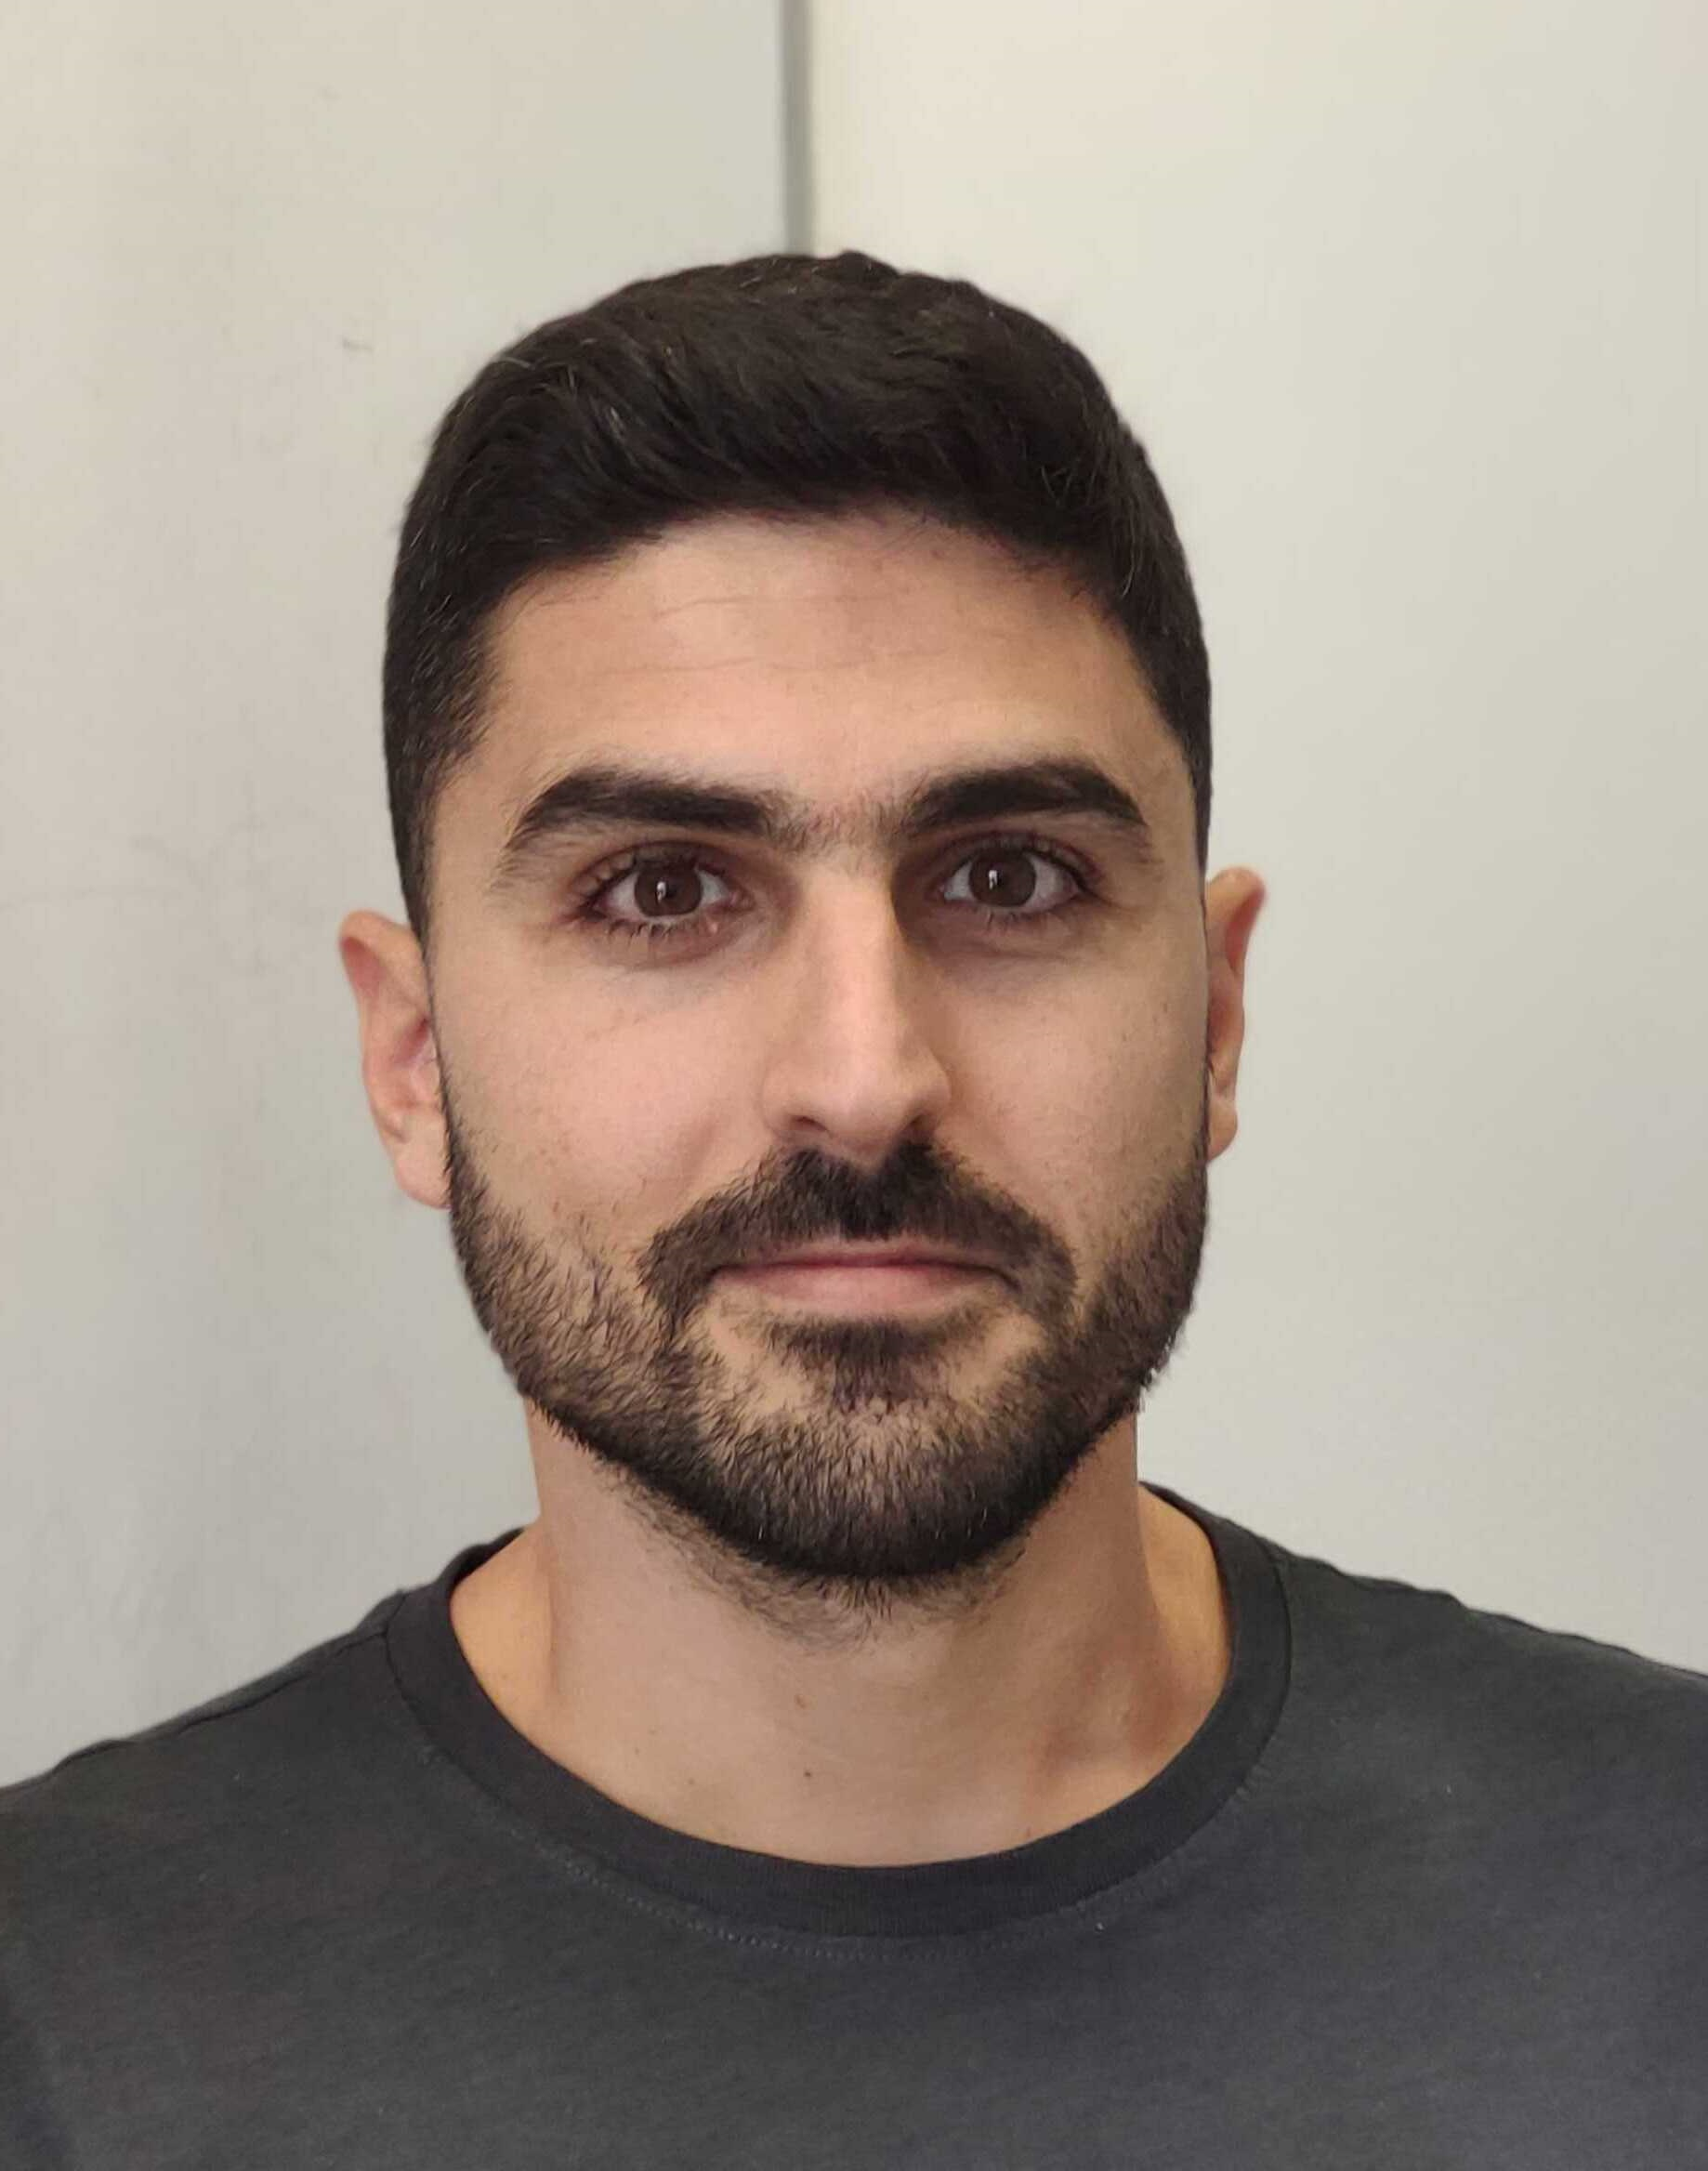
\includegraphics[width=1in,height=1.25in,clip,keepaspectratio]{Nikoletos-paper/profiles-pics/efthymiou.png}}]{Vasilis Efthymiou} is an Assistant Professor at the Department of Informatics and Telematics of Harokopio University of Athens (HUA), Greece. He received his PhD on the topic of entity resolution in the Web of data in 2017, from the Computer Science Department of University of Crete (UOC), Greece. Before joining HUA, he was a postdoctoral researcher at the database group of IBM Research in Almaden Research Center, CA, USA, a postdoctoral researcher at the Information Systems Laboratory of FORTH-ICS, Greece, and a visiting instructor at UOC. After his PhD research internship at IBM T.J. Watson Research Center, NY, USA, on matching Web tables to Knowledge Graphs (KGs), he has been co-organizing the SemTab challenges at ISWC, an effort to benchmark systems dealing with the tabular data to KG matching problem, and the Tabular Data Analysis (TaDA) workshop at VLDB. He has co-authored two books, more than 70 papers, and co-invented four US patents. 
\end{IEEEbiography}
\vspace{-30pt}
\begin{IEEEbiography}
[{
\includegraphics[width=1in,height=1.25in,clip,keepaspectratio]{Nikoletos-paper/profiles-pics/papadakis.png}}]
{George Papadakis} is a senior researcher at the University of Athens. He has also worked at the NCSR ``Demokritos'', the National Technical University of Athens (NTUA) and the ``Athena'' Research Center in Greece and at the L3S Research Center in Germany. He holds a PhD in Computer Science from Leibniz University of Hanover and a Diploma in Electrical and Computer Engineering from NTUA. His research focuses on web data mining.
\end{IEEEbiography}
\vspace{-30pt}
\begin{IEEEbiography}[{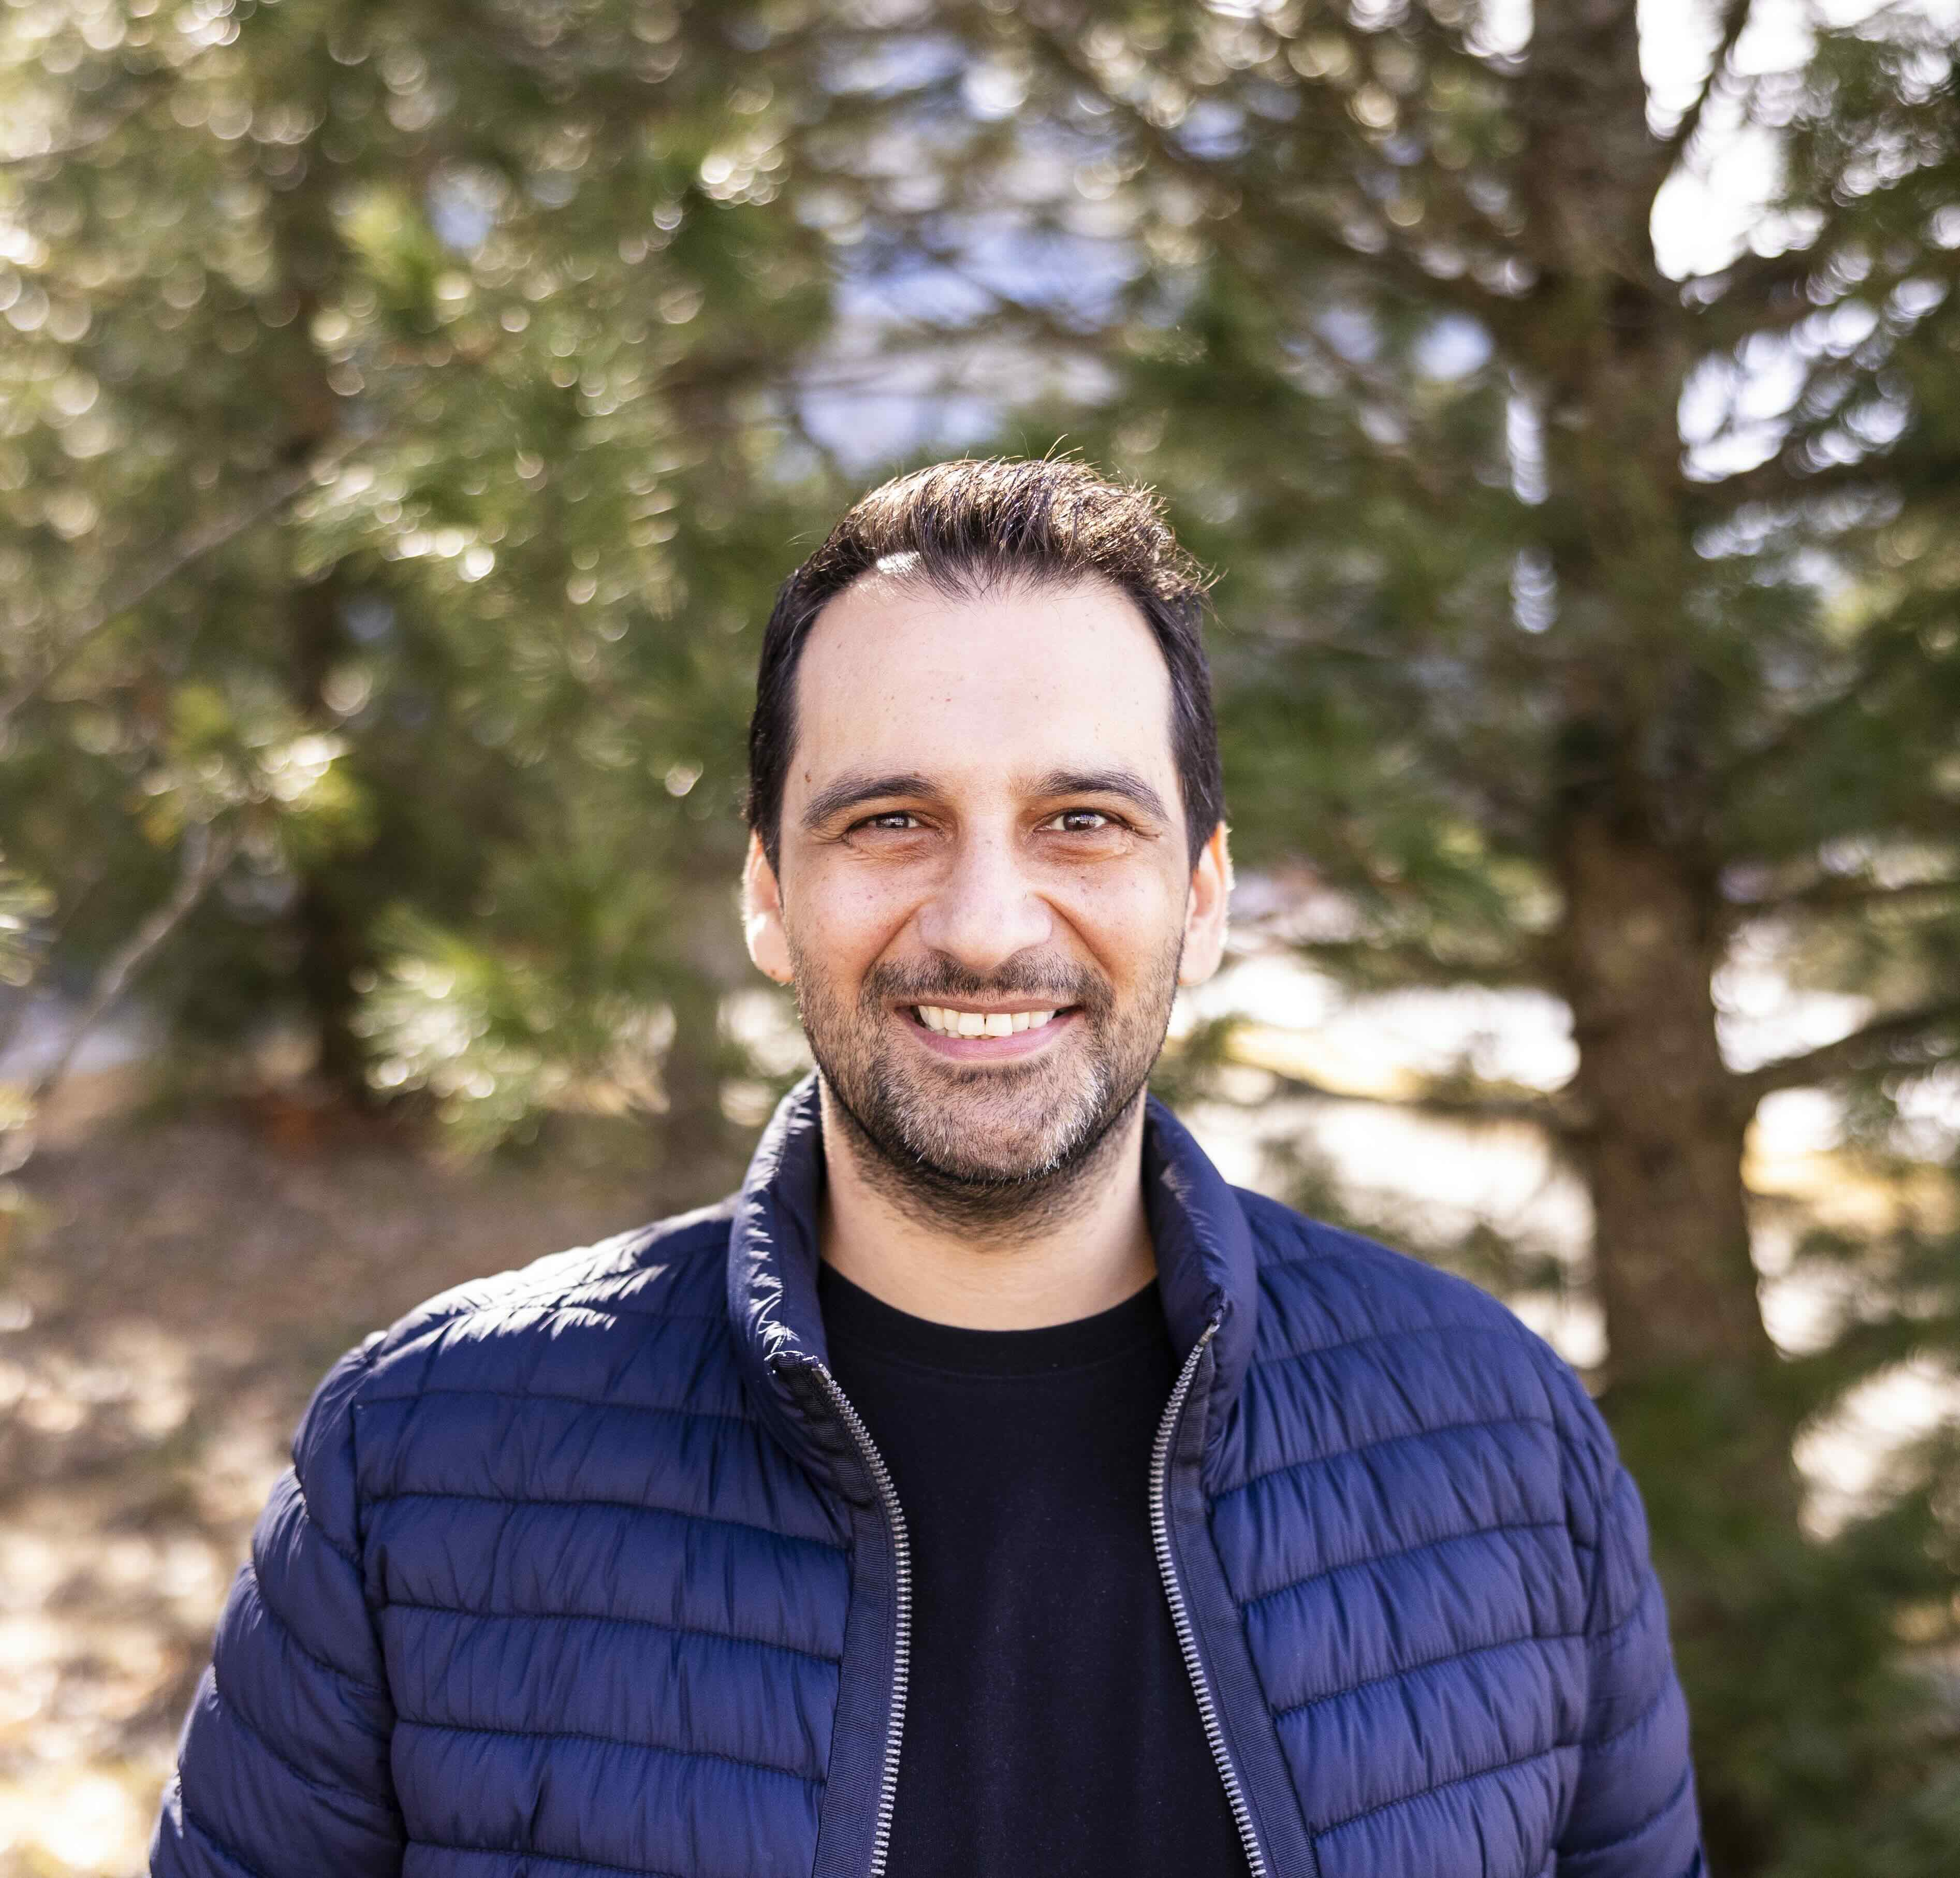
\includegraphics[width=1in,height=1.25in,clip,keepaspectratio]{Nikoletos-paper/profiles-pics/stefanidis.jpg}}]{Kostas Stefanidis}is a Professor on Data Science at the Faculty of Information Technology and Communication Sciences of the Tampere University in Finland, where he also leads the Data Science Research Centre and the Group on Recommender Systems. He has more than 10 years of experience in different roles at ICS-FORTH in Greece, NTNU in Norway and CUHK in Hong Kong. He received his Ph.D in personalized data management from the University of Ioannina in Greece. His research interests include the broader area of big data. His work focuses on personalization and recommender systems, entity resolution, data exploration and data analytics, with a special focus on socio-technical aspects in data management such as fairness and transparency, and has been published in more than 100 papers in top-tier conferences and journals. He has been involved in several international and national research projects, and is also actively serving the scientific community. Currently, he is the General co-chair of the ADBIS 2025, TPDL 2025, and EDBT/ICDT 2026.
\end{IEEEbiography}

\EOD

\end{document}